\documentclass{report}

\usepackage{style/suthesis-2e}

\usepackage[fleqn]{amsmath}
\usepackage{amssymb}
\usepackage{bm}
\usepackage{booktabs}
\usepackage{epigraph}
\usepackage{float}
\usepackage{graphicx}
\usepackage{listings}
\usepackage{mathrsfs}
\usepackage{natbib}
\usepackage{relsize}
\usepackage{subcaption}
\usepackage{url}
\usepackage[hidelinks]{hyperref}
\usepackage{refcount} % allows getting around stupid issues with references in headers + upercasing

\usepackage{tikz}

\usetikzlibrary{shapes,arrows}
\usetikzlibrary{decorations.pathreplacing, decorations.pathmorphing, snakes, calligraphy}

\tikzstyle{block} = [rectangle, draw, thick, align=center, rounded corners]
\tikzstyle{boundingbox} = [thick, lightgray]
\tikzstyle{dashblock} = [rectangle, draw, thick, align=center, dashed]
\tikzstyle{conc} = [ellipse, draw, thick, dashed, align=center]
\tikzstyle{netnode} = [circle, draw, very thick, inner sep=0pt, minimum size=0.5cm]
\tikzstyle{relunode} = [rectangle, draw, very thick, inner sep=0pt, minimum size=0.5cm]
\tikzstyle{line} = [draw, very thick, -latex']
\tikzstyle{arrow} = [draw, ->, thick]

\def\checkmark{\tikz\fill[scale=0.4](0,.35) -- (.25,0) -- (1,.7) -- (.25,.15) -- cycle;}

\definecolor{bpurp}{HTML}{984ea3}
\definecolor{bblue}{HTML}{377eb8}
\definecolor{bgreen}{HTML}{4daf4a}
\definecolor{borange}{HTML}{ff7f00}


% footnote without a marker
\makeatletter
\def\blfootnote{\gdef\@thefnmark{}\@footnotetext} 
\makeatother

\lstset{language=Python,
    frame=single,
    breaklines=true,
    postbreak=\raisebox{0ex}[0ex][0ex]{\ensuremath{\color{red}\hookrightarrow\space}}
}

\restylefloat{figure}
\newcommand{\Prop}{\textbf{Proposition: }}
\newcommand{\Prob}{\textbf{Problem: }}
\newcommand{\Prf}{\textbf{Proof: }}
\newcommand{\Sol}{\textbf{Solution: }}
\newcommand{\grad}{\nabla}
\newcommand{\Nats}{\mathbb{N}}
\newcommand{\Ints}{\mathbb{Z}}
\newcommand{\Rats}{\mathbb{Q}}
\newcommand{\Reals}{\mathbb{R}}
\newcommand{\Comps}{\mathbb{C}}
\newcommand{\Prb}[1]{P\left( #1 \right)}
\newcommand{\PT}[1]{P\left( \text{#1} \right)}
\newcommand{\PCon}[2]{P\left( #1 \mid #2 \right)}
\newcommand{\PConT}[2]{P\left( \text{#1} \mid \text{#2} \right)}
\DeclareMathOperator{\E}{\mathbb{E}}
\DeclareMathOperator{\tr}{\textbf{tr}}
\DeclareMathOperator*{\argmin}{argmin}
\DeclareMathOperator*{\argmax}{argmax}
\newcommand{\thus}{\quad\mathlarger{\mathlarger{\mathlarger{\Rightarrow}}}\quad}
\newcommand{\wght}{\mathbf{w}}
\newcommand{\im}{\text{im }}
%%\newcommand\scalemath[2]{\scalebox{#1}{\mbox{\ensuremath{\displaystyle #2}}}}


\usetikzlibrary{shapes,arrows}

\tikzstyle{block} = [rectangle, draw, thick, align=center, rounded corners]
\tikzstyle{boundingbox} = [very thick, dotted, gray]
\tikzstyle{dashblock} = [rectangle, draw, thick, align=center, dashed]
\tikzstyle{conc} = [ellipse, draw, thick, dashed, align=center]
\tikzstyle{netnode} = [circle, draw, very thick, inner sep=0pt, minimum size=0.5cm]
\tikzstyle{relunode} = [rectangle, draw, very thick, inner sep=0pt, minimum size=0.5cm]
\tikzstyle{line} = [draw, very thick, -latex']



\dept{Psychology}

\begin{document}
\title{Transfer and flexibility in humans and machines}
\author{Andrew Kyle Lampinen}
\principaladviser{Jay McClelland}
\firstreader{Noah Goodman}
\secondreader{Surya Ganguli}
%\thirdreader{Jane Supernumerary} %if needed
%\fourthreader{Severus Snape} %if needed

\beforepreface
\prefacesection{Abstract}

\afterpreface

\chapter{Introduction} \label{chapter:introduction}
\epigraph{``The most elementary single difference between the human mind and that of brutes lies in this deficiency on the brute's part to associate ideas by similarity.''}{William James, \textit{Principles of Psychology}}
Deep learning methods have achieved incredible success recently, reaching human-level performance in domains ranging from vision \citep[e.g.][]{Szegedy2015} to playing games \citep[e.g.][]{Silver2016}. However, these systems still lack some important human abilities \citep[e.g.][]{Lake2016}. Deep learning models are data-hungry, while humans can frequently learn from relatively few examples. Furthermore, even if they are given a large amount of data, deep learning systems may not be able to generalize well outside the data distribution they trained on. Finally, once knowledge is learned in the weights of a deep learning model, it is difficult to flexibly reuse that knowledge. From the perspective of William James (quoted above), most neural networks are brutes, which don't understand the similarity of new situations to their prior experiences, and so do not know how to flexibly respond to changes in their environment or goals. \par
By contrast, humans can use our knowledge flexibly. We can learn from few examples. We can introspect about our learned behavior to explain or change it. We can even remap our behavior in a way completely inconsistent with our prior behavior, such as trying to lose a game we have previously been trying to win \citep{Lake2016}. More generally, we are often able to accurately behave according to linguistic instructions without seeing examples of such behavior. All of these types of flexibility can be quite difficult for deep learning systems. \par 
This apparent contrast between humans and neural networks has raised questions about the validity of neural networks as a cognitive model for many years \citep[e.g.][]{Fodor1988}, and the recent successes of deep learning have only increased the frequency of these critiques \citep[e.g.][]{Lake2015, Lake2016, Lake2017, Marcus2018}. It is important to address these perspectives, and to understand how deep learning systems can be improved to serve as better models of human flexibility. There have been a number of attempts to address or integrate these critiques from a variety of perspectives \citep[e.g.][]{McClelland1999, McClelland2010, Hill2019a}. In this paper, I will focus on how these critiques overlook the benefits of transfer \citep{Lampinen2017a} and recent progress in deep learning \citep{Hansen2017}. In particular, deep learning research has made important progress on improving learning speed, generalization, and flexibility. However, even with contemporary methods there are many human-like abilities that remain frustratingly out of reach. \par
In this chapter, I will first review some of the cognitive issues and the progress to date, and try to provide a unifying perspective on how various types of transfer contribute to human learning and flexibility, by reviewing my prior work as well as that of others. In the remainder of this paper, I will present a new perspective on deep learning that builds off some of this recent work, and provides a technique for achieving more human-like flexibility in deep learning. \par

\section{Cognitive flexibility \& generalization}

What kind of flexibility do humans have? We are often able to learn rapidly. For example, we can achieve some competence in a novel video game within a few minutes \citep{Lake2016}. We can learn new concepts from seeing only a relatively small number of examples \citep[e.g.][]{Bourne1970}. We can often learn even faster if we can actively participate in the learning process by selecting examples rather than passively receiving them, especially if the concepts are simple enough that we can generate a good hypothesis space \citep{Markant2014a}. \par
We can then apply what we have learned to new situations. The studies of \citet{Bourne1970} show that, not only can people generalize to new examples of a concept they have learned, they can also transfer that knowedge to learn structurally-similar new concepts more rapidly. Indeed, even without explicit awareness of the relationship between two tasks, humans can sometimes benefit from transfer effects \citep[e.g.][]{Day2011}. In general, human analogical transfer abilities have been suggested to be a critical component of `` what makes us smart'' \citep{Gentner2003}. \par
Yet human flexibility is apparent beyond transfer between isomorphic tasks. We can often competently change our learned behavior in response to instruction or other goals, such as trying to lose a game we were previously trying to win, or trying to achieve some orthogonal task \citep{Lake2016}. Indeed, it has been known for almost a century that even other animals exhibit this sort of flexible knowledge use --- they engage in ``latent learning'' of environmental features that may be useful when solving future tasks \citep{Blodgett1929}. Both humans and other animals are capable of flexibly applying our knowledge in many situations.  \par
However, our flexibility is not universal. Sometimes it is quite difficult for us to integrate new knowledge. For example, even undergraduate students with substantial mathematical background often struggle with understanding new mathematical concepts.\footnote{I will focus on mathematical cognition in some places within this paper. Although the phenomena I discuss are much more general, and I will include a number of other examples, mathematical cognition offers a unique microcosm of human abilities for transfer, abstraction and flexibility.} They may mistakenly assume the converse of a theorem, or get caught up in concrete ways of thinking about abstract concepts \citep{Hazzan1999}. Socrates' dialog about doubling the area of a square captures the misunderstandings that modern subjects make, just as it did for those over 2000 years ago, yet it does not help them to deeply understand the principle \citep{Goldin2011}. Even after engaging with the dialog, nearly 50\% of modern subjects failed at the simplest generalization of the principle: to a square of different size. Similarly, even students who complete a course in geometry in high school may not achieve formal deductive understanding of the concepts taught unless (or until) they become undergraduate mathematics majors \citep{Burger1986}. Furthermore, superficial details of how a concept is presented can have profound impacts on how easy it is to reason about, even if the underlying concept is exactly the same \citep[e.g.][]{Kotovsky1985, Kaminski2008, Lampinen2017b}. There is a wealth of research showing that our learning is far from universally flexible. \par 
We also often fail to flexibly use the knowledge we have. For example, even mathematics students who can correctly state a rule or theorem are not necessarily able to apply it to create a proof \citep{Weber2001}. Similarly, even if experimental subjects can learn a basic concept rapidly, it may be difficult for them to apply it in more abstract situations or to extract more formal understanding from it \citep[e.g.][]{Lampinen2017b}. Likewise, rapid analogical transfer is often only possible when superficial details match closely, or when subjects are explicitly told to transfer \citep[e.g.][]{Gick1980}. Because of findings like these, \citet{Detterman1993} has argued that inducing transfer requires manipulations ``with the subtlety of a baseball bat,'' and so we should conclude that ``significant transfer is probably rare and accounts for very little human behavior.'' This is a particularly tendentious presentation of the issues, but it captures the important broader insight that humans are not always rapid learners or flexible reasoners. \par 
How can we reconcile the demonstrations of rapid learning and flexibility with the evidence that some concepts are learned slowly and some knowledge is inflexible? How can we reconcile arguments that transfer is key to ``what makes us smart'' \citep{Gentner2003}, with arguments that ``significant transfer is probably rare and accounts for very little human behavior'' \citep{Detterman1993}? There are a variety of factors that affect whether transfer will occur \citep{Barnett2002, Lampinen2017a}. First, we need high-quality representations of the concepts we are learning in order to reason flexibly with them. These generalizable representations are generally created through making connections between different pieces of our knowledge \citep{Wilensky1991, Schwartz2015}. Second, we often need strategic meta-knowledge about where and how to apply our knowledge in new situations, which also must be learned \citep{Weber2001}. Both these factors mean that transfer may happen more easily over longer periods of time, as I have argued in my prior work \citep{Lampinen2017a}. The quality of the representations we have, and the way those representations relate to the new tasks we are presented with, both affect our ability to learn rapidly, reason flexibly, and generalize. \par 

\subsection{Flexibility as transfer}
I argue that all these types of flexibility (and inflexibility) can be seen as transfer, defined broadly as the way that ``knowledge acquired in one situation applies (or fails to apply) in other situations.'' \citep{Singley1989}. From this definition it is clear that applying learned features and structures to learn faster in a new situation, as in \citet{Bourne1970}, is a type of transfer. I argue that in fact all rapid learning must rely on transfer of prior knowledge in order to constrain the hypothesis space under consideration\footnote{This is a consequence of the ``No Free Lunch'' Theorem \citep{Wolpert1996}, which shows that a learning algorithm cannot be \emph{a priori} better at generalizing than any other, including seemingly adversarial ones like choosing the model with the \emph{worst} validation error. The advantages of a learning algorithm can only be due to the match between its inductive biases and the structure of the task(s) it is used to learn.}. Even other types of flexibility, such as adapting to instructions, can be seen as transferring several different types of knowledge (prior knowledge about a task, other related taks, and language) to a new situation. For example, if we are asked to try to lose at chess, we are essentially presented a new task to which we need to transfer both our prior knowledge of chess and our prior knowledge of what ``trying to lose'' means. Thus flexibility and transfer are essentially two perspectives on the same broad phenomena. I will therefore use these words for different perspectives on this phenomenon. Specifically. I will use ``flexibility'' generally to refer to the behavioral phenomena, and ``transfer'' to refer to the computational principles underlying these phenomena. \par  
Why do we sometimes fail to be flexible? There are several reasons this can occur. First, we may not have the prior knowledge necessary to be flexible. We can't transfer what we don't know. Second, our representations may lack the quality necessary to transfer them. We often can't transfer what we don't know well \citep[c.f.]{Hazzan1999, Weber2001}. Third, we may not recognize that we have applicable prior knowledge to transfer \citep{Detterman1993}. Finally, we may actually have prior beliefs that do not apply to the present situation, and so transferring them will actually interfere with our ability to learn. This is generally called ``negative transfer'' \citep{Singley1989}. \par
For transfer to be beneficial overall, we must generally encounter settings where our prior knowledge is applicable, and furthermore we must have good ways of integrating that prior knowledge with new experiences. In the next section I will discuss some of the features that allow us to do so. \par

\section{What factors contribute to our flexibility?}
We need to address the computational question of how and when we can use transfer to behave flexibly. In this section I will give a brief overview of the contributing factors. \par 

\textbf{Complementary learning systems:} First, it has been proposed that we have complementary learning systems \citep{McClelland1995, Kumaran2016}. These complementary systems allow us to learn rapidly from new knowledge while avoiding catastrophic interference \citep{McCloskey1989} with the statistical knowledge we have accumulated over longer timescales. The key idea is that we have a slow (parametric) learning system which sets up good representations, while a fast (nonparametric) learning system stores new knowledge by using these representations. Throughout this paper, we will return to this theme of fast and slow learning which support each other. I will therefore divide the rest of this section into the ``slow'' and ``fast'' systems that contribute to transfer.\par
However, it's worth noting that ``slow'' vs. ``fast'' learning systems is not a strict dichotomy. This broad distinction is useful, but in reality learning systems fall on a continuum, and the time-course of learning in a given system is often dramatically affected by what knowledge is already present \citep[e.g.][]{McClelland2013}. Thus this dichotomy between learning systems should not be interpreted as a strict division. Instead, it is a useful way of highlighting the cooperation between distinct systems that operate across distinct, yet sometimes overlapping, timescales. \par 

\subsection{Slow}
In this section I will discuss the slow learning systems that contribute to transfer and flexibility. \par
\textbf{Culture \& education:} One critical contributor to transfer is culture. Our cultures have accumulated knowledge over extremely long time scales that allows us to advance much more rapidly now \citep{Tomasello1993, Bengio2012}. For example, mathematical concepts have been constructed by humans \citep{Hersh1997, MacLane1986}, and it has taken us millenia to construct subjects like calculus. Yet today many students gain fluency with these ideas before they graduate high school. Because culture has set up useful representations for these concepts, we are able to acquire them much more rapidly \citep[e.g.][]{McClelland2016}. Furthermore, culture has set up systems of education that are structured precisely to help us learn rapidly and generalize effectively. \par 
By contrast, if our culture does not represent or highlight certain concepts, we may struggle to reason about them. For example, one Amazonian tribe that lacks words for exact numbers shows substantially impaired ability to do basic tasks involving cardinality, which are interpreted as a fundamental deficit in the ability to represent exact cardinality at all \citep{Gordon2004}. Similarly, although the number line as a spatial representation of number appears relatively universal, cross-cultural and historical studies reveal that it is constructed rather than innate \citep{Nunez2011}. Culture helps set up powerful representations and metaphors for us to learn from. Without these representations, our learning would be substantially slower. \par 
\textbf{Transfer between tasks:} Even if culture has not explicitly highlighted (or engineered) structural relationships between tasks, we can benefit from structural similarity. For example, after learning an artificial grammar, subjects can generalize their knowledge to novel sequences from the same grammar applied to novel symbols \citep[e.g.][]{Tunney2001}. From learning about simple harmonic oscillators in the context of springs, participants can transfer to a superficially unrelated problem about controlling the population of a city \citep[e.g.][]{Day2011}. Because many tasks we perform share deep underlying structures, we can take advantage of transfer to learn faster on new tasks. \par 
\textbf{Grounding, embodiment, and representation quality:} One particular type of transfer that seems to be especially useful is grounding \citep{Barsalou2007}. In particular, conceptual representations often tend to be tied into more basic perceptual-motor systems, e.g. arithmetic in the Approximate Number System \citep{Park2013}, or mathematical (and other) reasoning in gestures \citep{Goldin-Meadow1993, Goldin-Meadow1999}. Indeed, the way we talk about many important abstract concepts, such as time, seems to be fundamentally tied to metaphors to more concrete concepts such as space \citep{Lakoff1980}. This sort of grounding can be very beneficial to understanding \citep{Nathan2008, Schwartz2015, Wakefield2018}. Because our perceptual-motor system have exceptionally good representations that are trained over long developmental time-scales, we may benefit from leveraging these representations to transfer our understanding to analogous conceptual domains. \par 
It is also worth considering that grounding and embodiment can hold us back. Even our understanding of symbolic expressions seems to be influenced by ``meaningless'' perceptual details like their spacing \citep{Landy2007}. It has also been argued that too concrete of examples can limit generalization \citep{Kaminski2008}, although the details of that particular demonstration have been debated \citep{DeBock2011, Lampinen2017b}. There is probably some negative transfer from grounding in some cases, but overall it is probably outweighed by the positive. \par
However, there are a number of conceptual issues that come along with grounding, such as how to define abstraction \citep{Dove2016}, and whether the grounding must be in the real-world, or can more generally be in concepts that are better understood \citep{Wilensky1991}, regardless of whether they are basic perceptuo-motor knowledge. The line between grounding and other types of transfer can be blurry, because, like many psychological ideas, its definitions are multifarious. \par 
The overlapping field of embodied cognition has raised the opposite issue, arguing that cognition cannot be considered at all outside of the physical, physiological, and social situations in which it is grounded \citep{Anderson2003}. Others have argued that even the computation metaphor in cognition is fundamentally flawed, because it neglects the fact that intelligence evolved in systems interacting with the world \citep{Cisek1999}, through a process of hierarchically constructed control systems \citep{Cisek2019}. The fact that many of our basic concepts seemed to be formed at the optimal level for action \citep{Rosch1976} has been cited as evidence for this \citep{Lakoff1999}. It is important to keep these arguments in mind, and not to neglect the world in which our brains reside in favor of a disembodied, computational mind. \par 
\textbf{Rerepresentation and different kinds of knowledge:} The work of Karmiloff-Smith \citep[e.g.][]{Karmiloff-Smith1986, Karmiloff-Smith1992, Clark1993} focused on the idea that we repeatedly redescribe our internal knowledge, reorganizing it in order to better understand the world. To support this theory, she examined evidence of U-shaped developmental curves, where children would actually get worse at a task before they reached ceiling, often because they at first over-generalized a rule. She argues that this shows a pattern of systematic progression of knowledge from implicit representations to various stages of explicit ones which allow progressively more flexibility. In \citet{Karmiloff-Smith1986} she describes some particularly interesting evidence: children fail to balance an oddly shaped block when asked to do so, but successfully balance it when asked to build a house, because their procedural knowledge is more sophisticated than their explicit knowledge. \par 
This pattern of procedural knowledge proceeding more explicit or object-like knowledge is supported by a much broader literature, from the gesture results of \citet{Goldin-Meadow1993} referenced above to work suggesting that we progress from understanding mathematical concepts as processses to understanding them as objects \citep{Dubinsky1991, Hazzan1999}. If we do not already have good representations for a concept, we must create them by slow, procedural learning and reorganization, before we can begin to reason flexibly with the concept. However, it's worth noting that the process is bidirectional --- procedural knowledge supports conceptual understanding, but conceptual knowledge also helps improve procedural performance \citep{Rittle-Johnson2001}. Furthermore, procedural learning can occasionally be misleading. Getting too caught up in procedures that only work in simple cases can actually inhibit conceptual understanding \citep{McNeil2005}. There are sometimes trade-offs to transfer (see section \ref{fast_slow_interactions}). \par 
Is a separate rerepresentation process necessary to explain these phenomena? It is difficult to determine this. Often rapid transitions and rule-like behavior can be fully captured within neural networks or statistical learning models more generally \citep[e.g.][]{McClelland1999, McClelland2002, Schapiro2009, Aslin2012}. While \citet{Karmiloff-Smith1992} argues that these mechanisms can not explain U-shaped developmental trajectories, since error-correcting learning will not apply where there are no errors, she ignores the potential effects of all the other learning that children are simultaneously doing on other related tasks. Furthermore, some compression emerges naturally from the learning dynamics of gradient descent \citep{Tishby2015, Shwartz-Ziv2017, Achille2017}, although there has been some debate about the generality of these observations \citep[][see]{Saxe2018a}. It is difficult to rule out the possibility that U-shaped developmental trajectories can be explained by the combination of compression and the effects of other learning on related tasks. \par
\textbf{Summary:} We accumulate knowledge throughout the course of our lives. Some of this knowledge is implicit in the statistics of the world around us, while some is culturally constructed and transmitted. The quality of our knowledge representations can be improved by connecting to other knowledge, or by grounding in perceptual-motor understanding. Once we have acquired sufficiently high-quality knowledge representations, we are often able to transfer when we encounter a new task, and thereby learn more effectively than we could from \textit{tabula rasa}. This improvement in learning manifests as both more efficient learning and better generalization. \par

\subsection{Fast}
In this section I will discuss the systems that contribute to fast learning and transfer. It's important to note that these are systems that can be applied rapidly, but are not necessarily learned rapidly. Indeed, many of these reasoning systems are themselves culturally constructed, and must thus be learned over development. \par
\textbf{Hippocampal:} From the complementary learning systems perspective, the hippocampus serves as a fast learning system which can store an essentially unlimited number of distinct experiences while minimizing interference, i.e. as a nonparametric learning sytem \citep{Kumaran2016}. This makes it an excellent sub-system for learning from a small amount of data, because it can store a few experiences and allow them to be retrieved at a later time. It can also help with integrating this knowledge without catastrophically interfering \citep{McCloskey1989} with knowledge gleaned from prior experiences, by allowing interleaving of these prior experiences in learning \citep{McClelland1995}. This can potentially occur in a usefully biased way \citep{Kumaran2016}. There may even be interesting computations performed within the hippocampus to support certain types of rapid generalization \citep{Kumaran2012}. \par 
\textbf{Interactive learning \& hypothesis testing:} Humans are able to use our stored experiences to rapidly learn. One example of this is that we often behave as though we are formulating and testing hypotheses, even from a very young age \citep{Sobel2004, Gopnik2014}. We can even take advantage of these hypotheses in order to actively acquire information from the world that is most useful for us \citep[e.g.][]{Markant2014a}. By using our prior knowledge of the world to help interpret new experiences, we are able to make extremely fast inferences about how to understand a new situation. \par
\textbf{Education \& learned flexibility:} However, our ability to reason rapidly is not solely learned on our own. Indeed, a focus of education is preparing us for future learning \citep{Bransford1999}, and flexibility \citep[e.g.][]{Richland2012}. That is, we are explicitly taught to learn increasingly rapidly as education goes on. Elementary school children require months or years of rote practice to learn arithmetic, but college mathematics students are expected to hear a theorem once and then immediately be able to apply it. As noted above, we may not be perfect at these faster learning tasks \citep[e.g.][]{Hazzan1999}. However, adults are much better at them than children, and mathematics graduate students are much better than undergraduates \citep{Weber2001}. The ability to learn and apply new knowledge rapidly develops as we do.Furthermore, as we grow up we also grow better at explaining our actions, and adapting to instructions \citep[e.g.][]{Doebel2015}. Over the course of development, we practice many types of flexibility. \par 
\textbf{Explanations and demonstrations:} Both in education and outside of it, explanations are a key way we learn about the world, because they can succinctly convey rich structure \citep[e.g.][]{Keil2006, Lombrozo2006}. Importantly, explanations can be succinct because they exploit our prior knowledge in order to convey only the information that needs to be clarified (i.e. they follow the pragmatic principle of not being overinformative, expressed by \citet{Grice1975} for communication more generally). We not only learn from hearing explanations, but also from producing them \citep{Chi1989, Chi1994}, and so it is a common pedagogical principle to ask students to generate explanations. Explanations form a key tool for learning. \par
Similarly, we can also learn quite rapidly from demonstrations, which provide another succinct means for conveying important structure in the world. This learning requires applying our prior knowledge to infer what should and should not be generalized, but fortunately we can do this even from a young age, see \citet{VanDamme2002} for example. Both explanations and demonstrations provide powerful tools for learning rapidly. We develop the ability to exploit these tools early in life \citep{Carpenter2005}. \par 
\textbf{Analogical and relational reasoning, and abstraction:} Some researchers have argued that analogical transfer and abstraction form crucial components of our learning \citep[e.g.][]{Gentner2003, Lakoff1980, Gentner2017}. These accounts often focus on fast, explicit transfer of the form explored by \citet{Gick1980}, for example. The structure-mapping algorithm \citep{Falkenhainer1989} proposed for this is based on explicitly searching over possible isomorphisms, which tends to be infeasible in practice. However, there may be ways to implement it efficiently enough that it could be considered for complex cognitive models \citep{Forbus2017}, and in past work I suggested that implicit learning could provide heuristics to dramatically speed up this search \citep{Lampinen2017a}. It's also reasonable to expect this ability to be related to education and other individual factors, since its been observed that features such as fluid intelligence may interact with the type of scaffolding provided to affect explicit analogical transfer \citep{Kubricht2017}. Indeed, older students are often better at transferring knowledge than younger ones \citep[e.g.][]{Chen1999}. This is suggestive of this type of transfer being a learned skill, rather than a cognitive primitive. \par
Much of the work on analogical and relational reasoning also focuses on the benefits of comparing multiple examples, which can lead to more reliable induction of abstractions or schemas and better transfer \citep{Gick1980, Gentner2017}. It has even been suggested that this is a key way to understand the benefits of grounding \citep{Jamrozik2016}. However, in some past work, I found that seeing two different presentations of a mathematical concept lead to better learning overall than seeing either individually, but did not lead to significantly better abstraction of formal principles \citep{Lampinen2017b}. Thus it remains important to ask when reasoning about multiple examples leads to abstraction, and when it does not. One feature that is often important is explicitly considering the relationship between examples \citep{Gentner2017}, but it's likely that the quality of understanding of the examples matters as well. \par 
\textbf{Consciousness and explicit reasoning:} Consciousness is a slippery topic, but unfortunately must be discussed, as it underlies many of the fast-learning systems above. Most of these rely on our ability to explicitly reason about concepts once we have sufficiently high-quality representations of them. The global workspace theory of consciousness \citep{Baars2005, Dehaene2017} is closely aligned  to this perspective. It states that conscious knowledge is precisely that which is globally accessible, and therefore with which we are most flexible. (C.f. also the higher-order-thought theory of consciousness \citep{Rosenthal1990}). This concords to some degree with the perspectives of \citet{Karmiloff-Smith1986}, who argued that once we re-represent knowledge to be explicit, we can use it more flexibly. \par
However, \citet{Karmiloff-Smith1986} also argued that there were different levels of explicit representation of knowledge, and indeed some consciousness researchers have proposed more graded transitions from implicit to explicit \citep[e.g.][]{Cleeremans2002}. Computational models of graded transistions have been proposed, where explicit knowledge is essentially learned by a separate system which reasons over implicitly learned representations \citep{Cleeremans2014}. This fits more with the work reviewed above showing a graded transition to explicit knowledge built upon implicit understanding grounded in percetual-motor features \citep[e.g.][]{Goldin-Meadow1993}, procedures \citep[e.g.][]{Hazzan1999}, or more basic concepts \citep{Wilensky1991, Patel2018}. Thus, when thinking about the relationship between implicit and explicit knowledge is unavoidable, we will take the perspective that explicit reasoning is built upon implicitly learned representations. \par 
Another place where explicit reasoning plays a role is in helping us to understand and learn from our own mistakes. For example, \emph{deliberate practice} (targeting specific aspects of performance for improvement) has been claimed to be key to developing expertise \citep{Ericsson1993, Ericsson2017}. Yet to engage in deliberate practice requires meta-knowledge about what needs to be improved, and indeed this abstract understanding is an important component of expert knowledge \citep{Feltovich2012}. \par
\textbf{Summary:} We possess fast learning systems that are engineered by evolution, such as the hippocampus, and ones that are culturally transmitted, such as our ability to follow instructions in our native language(s). Together, they allow us to infer a great deal from little information, by leveraging our slowly-accumulated prior knowledge. They also allow us to flexibly adapt our behavior through practiced algorithms like following instructions. \par 

\subsection{Interactions between fast and slow learning systems} \label{fast_slow_interactions}
I claim that most transfer arises as a synergy between different kinds of learning across different timescales. In particular, the knowledge we have accumulated over our lifetimes (part of which has been accumulated by our cultures over millenia) allows us to constrain the hypothesis space for new learning, so that we can make accurate inferences from a few examples in a new situation. \par 
From my perspective, this slowly-learned knowledge of the world can take multiple forms. It can occur in the mapping from inputs to our awareness, for example in visual cortex neurons which adapt to the regularities encountered over development \citep{Barlow1975}. However, it can also occur in the systems that implement higher-level and more rapid computations.\footnote{Clearly certain kinds of knowledge will lend themselves more easily to being learned in development and others will lend themselves more easily to being culturally transmitted or even learned by evolution. For the most part, I will generally assume that this knowledge emerges from experience or is culturally conveyed rather than being built in \citep{Hansen2017}, but my conclusions will mostly be agnostic to the origins of any particular piece of knowledge.} For example, the results on transfer in artificial grammar learning described above \citep{Tunney2001} or the results on transfer of simple harmonic oscillator strategies \citep{Day2011} show that humans are able to transfer knowledge at the level of structures or algorithms. The limits of this transfer are as yet unclear, as are the time-scales over which different kinds of transfer can occur; some of the work in my dissertation will attempt to explore these issues.\par  
\textbf{Limitations \& tradeoffs:} Of course, there are trade-offs to relying on transfer and prior knowledge. When new tasks are not well aligned with our prior knowledge, relying on prior knowledge can actually interfere with learning. For example, this is one piece of the argument that we made \citep{Lampinen2017b} to explain the results of \citet{Kaminski2008}. This is an illustration of the broader phenomenon of negative transfer --- interference effects produced by transferring between non-isomorphic domains. A wide variety of studies have observed this type of phenomenon \citep[e.g.][]{Luchins1942, Landrum2005}. Our prior knowledge can be detrimental in some situations. \par
This brings us back to the broader point raised by \citet{Detterman1993} above, that humans are often unable to efficiently or flexibly transfer knowledge to new situations. Instead, this must be a goal of education \citep{Bransford1999}, and learning what is transferable may require developmental time \citep{Lampinen2017a} if the representations of the tasks are not sufficiently good to support faster transfer. We can be efficient and flexible when our prior learning has set us up to be. We are not always. We can be mislead by mismatches between the past and the present, or we can simply fail to find the correct analogy.\par

\section{Steps towards flexibility in deep learning}

A great deal of recent work in machine learning can be seen as attempts to build machine-learning systems with greater flexibility. In particular, much of this work has tried to allow them to learn from fewer examples, or generalize better to data that weren't seen during training. This work typically follows one of two approaches. The first, multi-task learning, focuses on learning multiple tasks with a single model, in the hope that the additional constraints on the model's representations will cause it to learn more rapidly or generalize better. The second approach, meta-learning, focuses on learning how to learn tasks, in the hopes of learning much faster and generalizing better from extremely small samples. I will give a brief overview of both these literatures in this section. \par

\subsection{Multi-task learning}

Multi-task learning is generally related to the ``slow'' learning systems I described in humans. Typically, parameters are partially shared between the two tasks, and these shared parameters are learned over long time-scales. This can be done either in a sequential fashion (where you use one task to pre-train the network for another), or simultaneously (where you learn multiple tasks at the same time or on alternating gradient steps). Auxiliary tasks need not be of the same type as the main task, for example reinforcement learning tasks can be supplemented with auxiliary supervised tasks like temporal autoencoding \citep[e.g.][]{Hermann2017}, or unsupervised tasks can be used to pre-train for supervised ones \citep[e.g.][]{Wu2018}. \par
\textbf{Pre-training:} One example of sequential multi-task learning is the extremely common practice of pre-training a network on some canonical task in order to use one of its hidden layers as a feature for some other related task. For example, pre-training on ImageNet \citep{Deng2009} is often seen as a useful general feature extractor for vision tasks \citep{Huh2016}, even for quite different transfer domains \citep[e.g.][]{Marmanis2016}. There is still active research on how to optimally pre-train features for various goals \citep[e.g.][]{Wu2018}. \par    
However, pre-training is used on more than just vision tasks. In natural language processing (NLP) applications, the representations of words is often pre-trained on co-occurrence prediction tasks \citep[e.g.][]{Pennington2014}. The more general language modeling task (predicting words conditioned on past input) can serve as unsupervised pretraining for many tasks \citep[e.g.][]{Radford2019}. In AlphaGo \citep{Silver2016}, the networks were pre-trained to predict expert go-players' moves, and then were tuned from that starting point using reinforcement learning. For other RL tasks, various pre-training approaches can be useful, such as training the agent to be able to reach diverse states \citep{Gregor2016}, or trying to learn adversarially discriminable skills \citep{Eysenbach2019}. The principle that pre-training a network can allow it to generalize better from smaller training sets appears to be quite general, although there is still some debate and ongoing research \citep[e.g]{He2018, Silver2017}. \par
There are also many remaining questions about how other features of training interact with transfer. Some researchers have argued that \emph{disentangled} representations --- loosely those that represent distinct features in distinct subspaces --- will be helpful for future tasks \citep{Higgins2018}, while others have argued that disentangled representations are hard to define, and that the evidence that they are useful is weak \citep{Locatello2019}. Other some recent work suggests that some forms of regularization may actually harm transfer \citep{Kornblith2019}. One possible explanation for this is that regularization is too compressive in the transfer setting --- it may compress away some real features that are useful for the transfer task, but not for the source task. However, this might be different if the tasks were trained simultaneously (see below) rather than in a pre-training setting. Understanding when this occurs, and how to balance the generalization benefits of regularization with transfer benefits will be an important area for future work. \par

\textbf{Curriculum learning:} A more general kind of pre-training is curriculum learning \citep{Bengio2009} --- the idea that training models on a structured progression of tasks can improve generalization. Pre-training on a single task is essentially a very simple curriculum. The idea of curricula began with \citet{Elman1993}, but was debated \citep[e.g.][]{Rohde1997}. However, subsequent work has demonstrated the importance of curricula both in toy settings \citep{Gulcehre2013} and in much more complicated tasks and models \citep[e.g.][]{Zaremba2014, Graves2016}. \par
Of course, having to devise a curriculum for each task you want to perform requires substantial human effort, which has led to work on automated ways of deriving curricula \citep{Graves2017}. This is a difficult challenge --- while approaches like tracking progress on many tasks and training on the ones where performance is changing the most \citep{Baranes2013}, or adversarially generating tasks of intermediate difficulty \citep{Florensa2018} can work in simple domains, in more complex task settings the problem remains open. When the task consists of a two-player game, play between agents as they learn can form a natural curriculum --- the difficulty of the task increases precisely as the agent learns \citep{Silver2017, Jaderberg2019}. However, in more general non-competitive tasks, it is not clear how such an approach could help. \par 
In recent work, my collaborators and I explored a new approach to automated curriculum generation for goal-conditioned reinforcement learning \citep{Racaniere2019}. We combined several ideas from the previous work in novel ways in order to scale these approaches up to more complex tasks, and tackled novel challenges, such as automated curriculum generation in environments where the possible tasks vary between episodes. We also highlighted a challenge to naive approaches --- as the complexity of the task space grows, it becomes very inefficient to explore task space at random, or by uniformly increasing difficulty. Most tasks in a complex environment will not be useful for the ultimate goal; for example, teaching a self-driving car to do a flip might be difficult, but it would not help with most tasks we want the car to perform. Human curricula are designed to efficiently lead learners to the desired competency, and we drew inspiration from this to propose a novel technique for pulling curricula towards a desired task distribution. These results represent a substantial step towards automated curriculum derivation in environments closer to the complexity of the real world. However, as we highlight in the paper, in more complex tasks it can be difficult to generate a curriculum without auxiliary information about the environmental structure. This is where the cultural knowledge behind human curricula, and the systems of mutually supporting tasks we have developed, will likely be necessary for achieving human-level intelligence. \par 

\textbf{Continual learning \& avoiding interference:} Curriculum learning raises another issue --- what if you want your model to perform well at several tasks? If you switch to training on a new task, it may catastrophically interfere with your ability to perform a previous task \citep{McCloskey1989}. The complementary learning systems perspective \citep{McClelland1995, Kumaran2016} was intended in part to address this issue. A number of other approaches have also been proposed recently, based on ideas like preserving parameters from updates proportionally to how important they are for old tasks \citep{Kirkpatrick2016, Zenke2017}, or learning tasks separately but distilling the knowledge into a single network later \citep{Rusu2015}, or by trying to use unsupervised learning to find compact representations and allocate new tasks so that they don't interfere \citep{Achille2018a}. There are also some memory-based approaches discussed in section \ref{meta_learning_sec} that can ameliorate this problem. Thus there are a variety of approaches that can address catastrophic interference, while still maintaining the benefits of curriculum learning. \par
However, beyond avoiding interference, a major hope is that prior knowledge, even in dissimilar domains will help with learning of a new task. While most curriculum learning work at present still samples the curriculum from a very narrow set of tasks, such as navigation goals of varying difficulty \citep{Florensa2018}, humans seem to be able to leverage analogies from much more disparate domains, such as using the flow of water to understand the flow of heat \citep[][see]{Falkenhainer1989}. It remains a challenge for machine-learning systems to learn different types of knowledge from the variety of tasks that humans experience, in such a way that prior learning supports new learning rather than interfering with it \citep{Mitchell2018}. \par 

\textbf{Simultaneous multi-task learning:} Many multi-task learning approaches train on the tasks simultaneously rather than sequentially. For example, simultaneously training a natural language translation system to do image captioning in the target language improves its translation performance \citep{Luong2016}. Even training it to translate between multiple language pairs is beneficial \citep{Dong2015}. This can even lead to zero-shot generalization to translation between language pairs never seen together in training \citep{Johnson2016a}. \par 
The idea of multi-task learning has proven even more critical in Reinforcement Learning (RL), where auxiliary tasks have been suggested as a key approach to overcoming the problem of reward sparsity \citep[e.g.][]{LeCun2016}. They have been used this way on a variety of RL tasks, for example in grounded language learning \citep{Hermann2017}. \par
The broad observation that deep networks will learn representations that represent shared structure in the tasks they perform, and can exploit this shared structure to generalize better, is not new. It was observed at least as long ago as \citet{Hinton1986}, and has continued to intrigue researchers since \citep[e.g.][]{Lampinen2017a}. In particular, it is a key feature that separates deep networks from simpler statistical learning architectures, and allows them to uncover and exploit deep structure in the world \citep{Rogers2008}. This is key to some of the kinds of transfer that deep networks demonstrate, and has been substantially helpful in the machine learning work above. Thus the benefits of multi-task transfer should not be neglected when considering deep learning models of cognition. \par 

\textbf{Learning which parameters to share:} Most the work above simply fixes architectures with pre-specified shared and unshared weights. However, there are other approaches that attempt to learn which weights to share. The work of \citet{Achille2018a}, referenced above, is one example of this.  Other authors have considered using evolutionary algorithms to decide which subsets of modules should be shared \citep{Fernando2017}. Some other approaches can also be seen from this perspective, for example choosing a sparse subset of modules for each forward pass \citep{Shazeer2017} or using a HyperNetwork to generate the weights for other networks \citep{Ha2016}. Both these can be seen as a way of learning which weights should be shared or separate between different ``sub-tasks'' of a task. Some of the work discussed in section \ref{meta_learning_sec} can also be viewed as learning what parameters should be shared and which should be separate. While in principle a fully-shared network could learn which parameters to share just by gradient descent, in practice a more structured approach to this problem can be useful. \par 

\textbf{Tasks as an input feature:} The most flexible approach to multi-task learning involves simply providing task representations as an input to the model and letting everything be learned, rather than pre-specififying anything about how computations should be shared and separated. This has the benefit that the system can potentially learn to generalize to novel tasks. Research on general value functions in reinforcement learning \citep{Sutton2011} --- value functions which take a task specification as an input --- provide one inspiration for this. Task-conditioned RL approaches have exhibited success in certain cases, for example generalizing to unseen natural-language task specifications \citep{Hermann2017}.  \par

\textbf{Model-based reinforcement-learning:} Model-based RL methods provide a useful factorization of the RL task, that can allow the same model to be used for a new task with a different reward function \citep[e.g.][]{Laroche2017}. More flexible hybrid model-based methods, such as letting an agent learn to plan \citep{Tamar2017}, show potential promise. However, many of these suffer from stability issues, as prediction errors compound over rollouts \citep{Talvitie2014}. However, treating these rollouts as a potentially flawed imagination, and letting the model learn to interpret them can help \citep{Racaniere2017}, as can rolling out in latent space rather than in observations \citep{Gregor2019}. It seems likely that one component of flexibility will be learning models that can be reused for new purposes. However, it is as yet unclear what those models will look like, and whether they will need to have planning as an inductive bias at all. At least in some circumstances, planning-like behavior can emerge in a model-free architecture with an appropriate recurrent structure \cite{Guez2019}. \par

\textbf{Summary:} To summarize, curriculum and multi-task learning can help set up representations that allow deep learning models to generalize better from less data, or to learn tasks that would not otherwise be learnable. This is because the additional constraints imposed by auxiliary or pre-training tasks on the networks representations help it to uncover the true underlying structure in the world. While multi-task learning does not support all the kinds of flexibility that humans demonstrate, it is a key piece of the puzzle of how deep networks can learn faster and generalize better. \par

\subsection{Meta-learning \& related approaches} \label{meta_learning_sec}

The fundamental insight of meta-learning is that there is a continuum between data and tasks. We can interpret each (input, target) tuple as a simple task, and we can interpret subsets of a dataset as sub-tasks, for example all the dog images contained within ImageNet form a semantically distinguishable sub-task of the overall task. Analogously, we can often interpret a single task as being just a point in a larger space of tasks. Most meta-learning models exploit these insights by having the architecture adapt to a given task within its activations instead of its weights, just as a CNN would adapt to the fact that its current input was a dog image rather than a tree image within its activations. Learning to adapt to new tasks in this way has been shown to allow for much more efficient learning on new tasks, and may be key to modeling human intelligence \citep{Hansen2017}. \par 
\textbf{Basic meta-learning:}
The basic meta-learning approach (representing a task within activations) has been applied to many settings. For example, it has been used to learn to classify new images based on single positive exemplars of each class \citep{Vinyals2016, Ravi2017}. It has also been used to teach recurrent networks to solve simple reinforcement learning problems \citep{Duan2016, Wang2016a, Stadie2018}. \par
There have been many variations on this approach. Some meta-learning work has exploited both slow and fast weights with some success \citep[e.g.][]{Munkhdalai2017}, taking one perspective on the dichotomy I proposed above. Many approaches have exploited other tricks that are broadly useful in machine learning. For example, some work has leveraged unlabelled examples along with a few labelled ones to yield better meta-learning results \citep[e.g.][]{Ren2018}. Other work has shown that attention-based models are useful \citep{Reed2017}, as in many other machine-learning applications \citep[e.g.][]{Vaswani, Gregor2015}. \par
\textbf{Memory-based:} There are a variety of meta-learning approaches that are based on a non-parametric memory, and generally some form of key-value attentional lookup over it. A general extension of the basic meta-learning approach to the case with memory is given in \citet{Santoro2016}. Other approaches are based on using memory only at testing, e.g. by tuning the network rapidly to perform well on similar examples, as proposed by \citet{Sprechmann2018}. \par 
More flexible variants have also been proposed. For example, the differentiable neural computer (DNC), proposed by \citet{Graves2016} is able to receive a graph structure as inputs, learns to store it in memory, and then learns to use that stored information to solve problems like computing shortest paths. This can effecetively be seen as meta-learning --- the architecture has the flexibility to learn and reason from new knowledge rapidly. However, this flexibility remains fundamentally within the computations done for a task which is slowly learned, and does not by itself allow the more general flexibility that humans exhibit. \par
\textbf{Language:} There is some work that has explored related problems from a language-based perspective. For example, \citet{Larochelle2008} considered the general problem of behaving in accordance with language instructions as simply asking a model to adapt its response when conditioned on different ``instruction'' inputs. Later work explored zero-shot classification based on only a natural language description of the target class \citep{Socher2013,Romera-Paredes2015}. More recently, there has been a productive line of research in using language to compose network modules for question answering \citep{Andreas, Andreasa}. There has also been some work on reinforcement learning systems that learn to follow natural language instructions in a simple enviroment \citep{Hermann2017}. Other work has shown that language can form a useful intermediate representation for a simple form of hierarchical reinforcement learning \citep{Jiang2019}. \par
More recently, \citet{Radford2019} showed that a language model trained on an extremely large corpus of curated websites actually acquires some meta-like abilities, for example the ability to translate languages ``zero-shot'' (i.e. when conditioned on examples of translation pairs and then given a new sentence, it produces a translation). It is also able to summarize, answer questions, etc. It does this presumably because the corpus contains some translation pairs in context or summaries on a page, and so those tasks essentially compose a small part of the language modeling problem. It's worth noting that the performance on these tasks is rudimentary, and far from models that are trained for these tasks in a supervised way, but it is still an impressive demonstration of the power of prediction to extract deep latent structure in the world, and the power of broad enough training data distributions to teach flexibility. \par  

\textbf{Demonstrations:} The issue of learning from demonstrations has also been considered in the machine learning literature for some time, because of its potential applications in problems where we know what behavior we want, but not how to encode it. There the problem has generally been referred to as ``inverse reinforcement learning'' \citep{Ng2000}, i.e. the problem of inferring a value function from observed behavior. A large number of approaches to this problem have been proposed \citep[e.g.][]{Ng2000, Abbeel2004}. Recently, approaches combining meta-learning and deep learning have achieved some success on this. For example, \citet{Finn2016} present an algorithm which can learn to infer a reasonable approximation of the objective function from a single demonstration. This work shows that neural networks can learn to learn from demonstrations. \par
\textbf{Relational and analogical reasoning:} There are a number of other approaches that attempt to explicitly build relational priors or abstraction into deep-learning architectures. Relation networks \citep{Santoro2017} build in this prior by having the architecture explicitly relate different parts of the input, and achieve better performance on answering relational questions about visual scenes. Architectures that directly allow for true relational binding can be beneficial for a variety of applications, especially natural language processing or symbolic reasoning \citep[e.g.][]{Smolensky1990, Smolensky2014, Huang2017}. Graph-structured architectures form a very natural way of representing few-shot learning problems \citep{Garcia2018}, and more generally graph-structured or other relational inductive biases have been suggested as a promising direction in deep learning \citep{Battaglia2018}. How these inductive biases benefit (or limit) learning is an important direction for future research. \par 
However, relational reasoning is constrained by training as well as the architecture. For example, choosing the negative examples that a network learns from to explicitly contrast relational hypotheses can help to yield more relational reasoning \citep{Hill2019}. Exploring how architecture and training interact to produce relational reasoning will be an important future direction. \par
\textbf{Abstraction:} There has also been some work on explicitly building in abstraction capabilities to machine learning systems. For example, in reinforcement learning the idea of options \citep{Sutton1999} and hierarchical reinforcement learning more broadly \citep[e.g.][]{Botvinick2009} are essentially encapsulations of temporal abstraction, where a sequence of actions can be represented as a single higher-level action. For example, we can think of going to the office as a single action, rather than a sequence of many steps. Similar attempts have been made to allow deep learning models to share knowledge across tasks, with some success \citep[e.g.][]{Tessler2016}. \par 
There have also been a variety of attempts to combine deep learning methods with more programming-like approaches. For example, Neural Programmer-Interpreters \citep{Reed2015} essentially endow a recurrent network with the ability to call sub-routines, and a stack of memory for these sub-routines to use. Applying these ideas to meta-learning problems has been reasonably successful, especially with carefully chosen algorithms for integrating knowledge across tasks \citep[e.g.]{Devlin2017}. Similar techniques have been applied to many domains, such as learning from demonstrations \citep[e.g.][]{Xu2017a}. Combining the old ideas of cognition as executing symbolic programs \citep{Newell1961} with the techniques of deep learning can yield improvements in flexibility. \par  
However, most of these methods are still not as universally flexible as humans. The number of abstractions is usually fixed, often abstractions cannot be composed from other abstractions, and abstractions are inflexible to other demands. For example, a system that has learned an option for walking to a goal will not necessarily be able to change to running to the goal without learning this option from scratch. Thus there are still limitations to these approaches at present. \par 
\textbf{Other work:} There is a variety of other work that has exploited different perspectives on meta-learning. Some of this work could be useful for thinking about flexibility. For example, \citet{Finn2017a} proposed Model-Agnostic Meta Learning (MAML), an approach based on optimizing the model so that it could adapt well to a new task in a few gradient steps, and this work has led to many follow-ups \citep[e.g.][]{Finn2017, Finn2018, Nichol2018}. \citet{Xu2018} proposed using meta-learning to adapt hyperparameters of reinforcement learning algorithms across tasks. Other work has attempted to meta-learn auxiliary tasks for transfer, based on improvement on target tasks \citep{Liu2019a}. All of these approaches allow for better adaptation to new tasks or environments. \par
In addition, there has been some work showing that basic neural network models can adapt rapidly to new data that is consistent with prior knowledge, simply by optimizing weights specific to that data while freezing the remaining weights of the network \citep{Rumelhart1993}. This approach only works if there are weights that are specific to the new item(s), so it is not a general kind of flexibility. Nevertheless, this approach has been applied to understand human semantic cognition \citep{Rogers2004}. More recently, I applied it to one-shot and few-shot learning of words in a language-modeling task \citep{Lampinen2018a}. Thus under some circumstances this approach can yield a certain kind of flexibility, even at the scale of large machine learning tasks. This is more evidence of the general point that information which is consistent with prior knowledge can be rapidly integrated \citep{McClelland2013}. \par 
\textbf{Unintentional ``flexibility'':} There has also been some interesting work on flexibility that emerges accidentally under standard training of deep learning systems. In particular, adversarial examples \citep{SzegedyAdv} are cases when adding a very small perturbation to an input can radically alter the network's output. This is a kind of flexibility, but it is not the desired kind. Instead, these appear to be evidence for the fact that deep networks are inherently chaotic systems, which can respond in surprisingly sensitive ways to their inputs. However, it's worth noting that humans can be susceptible to more extreme adversarial perturbations derived on deep networks \citep{Elsayed2018}. Furthermore, adversarial examples can be exploited, e.g. for better training \citep{Goodfellow2015}. \par 
\citet{Elsayed} demonstrated an even more interesting type of unintentional flexibility: deep networks can be ``reprogrammed'' by an input to solve a different task.\footnote{Although not one completely unrelated to the main task the network was trained on --- the network was trained on a vision task, and their reprogrammed tasks were just other vision tasks. It would be interesting to explore the limits of this ``reprogrammability.''} This is a step closer to the flexibility that humans have, but the ``reprogramming'' inputs have to be derived via an optimization process, and tend to be uninterpretable. Thus there is no systematicity in this flexibility. However, my interpretation of these results is that they are encouraging evidence that these models have the capacity to be extremely flexible under appropriate conditions. All that is needed is to train this flexibility to be more systematic. \par  
\textbf{Summary:} To summarize, meta-learning has made progress on several fronts. It is starting to solve the small data problem, by allowing networks to learn efficiently from a small number of examples \citep[e.g.][]{Wang2016a}. At the other extreme of very large data, deep networks can generalize to some extent to tasks which are only hinted at by the trained task distribution \citep[e.g.][]{Radford2019}. However, there are a number of key features of human flexibility that remain to be explained. In the next section, I will relate transfer and flexibility in humans and deep networks, and discuss what features are still missing. \par 

\section{Relating flexibility in humans and neural networks}

The encouraging progress on multi-task and meta-learning in recent years suggests that cognitive models exploiting these techniques may help explain human flexibility and transfer \citep{Hansen2017}. In this section, I will attempt to relate the aspects of human and network flexibility that I outlined in the previous sections. \par 
First, it generally seems that the division between fast and slow transfer is applicable both to the machine learning literature (meta-learning vs. multi-task) and to human transfer, as we highlighted above \citep[and in prior work, namely][]{Lampinen2017a}. Following complementary learning systems, I suggest that broadly our slow learning of structure in the world happens over the course of developmental time in a multi-task fashion. Algorithmically, this occurs because parameters in our brain come to represent and exploit structural similarities across the many tasks we experience. We also practice doing fast learning over these slowly-learned representations, in educational settings as well as in everyday experience more broadly. Thus I think that cognitive models should employ both slowly-learned shared representations, and a system that allows for rapid and flexible reasoning over them. I argue that incorporating both aspects will be key to modeling the full range of human flexibility. \par 
It is also important to note the differences between the systematic, structured training that humans encounter in culturally-constructed educational systems, and the unstructured, IID training that deep learning models canonically receive. While curriculum learning addresses some of the sequential learning in education, and meta-learning addresses part of the learning-to-learn aspect, the full training on flexibility is generally missing. For example, humans learn a great deal from explaining as well as simply doing, yet we rarely train our machine learning models to explain their actions. Given the sensitity to training data that both humans and neural networks display, we cannot expect deep learning models to capture human behavior completely under drastically different learning regimes. How to train deep models in more human-like ways is an important direction for future work.  \par
In summary, I think deep learning models remaining promising cognitive models. They have successfully modeled a wide range of phenomena ranging from low-level neural activity to cognition. Furthermore, they are compelling models in particular of high-level cognitive phenomena, because they are some of the only systems to successfully achieve human performance at difficult tasks like visual recognition or playing go. They even have some inherent (if often unstructured and unintentional) flexibility, as indicated by adversarial examples and reprogramming. \par
I suggest that humans are similarly flexible. I suggest that the reason our flexibility is less chaotic is that we learn over the course of development and education to exploit our flexibility in systematic ways, in order to be adaptable to new tasks and situations. A very weak example of this in machine learning is given by \citet{Radford2019}, discussed above, where training a language model on a large enough text distribution gives some generalization to related tasks. However, this network required far more training than could be assumed for humans, and still lacked some of the flexibility that humans have. I suggest that this is because of the lack of multiple tasks to constrain the representations, the lack of an architecture explicitly designed to allow synergies between fast and slow learning, and the lack of the systematic, structured training at the scale that humans experience. \par 

\subsection{What's still missing?}

For the reasons highlighted above, some flexibility is still missing from deep-learning systems. Although they can often learn a new task from few examples, most demonstrations of this have involved sampling tasks that are within a dense region of the training task distribution. Furthermore, humans have a great deal more flexibility than simply learning rapidly. We can decide how to behave on a new task based on natural language instructions we are given. We can also adapt our behavior on a task based on feedback about our actions, and can jointly learn from language and examples better than we can learn from either alone. \par
We can also remap our behavior on tasks based on instructions or examples of tasks. For example, if we are told to try to lose a game we have previously been trying to win, this is an easy task for us. It would be quite difficult for any contemporary reinforcement learning model to invert its value function. If we are given examples of task mappings, e.g. we've played chess on a smaller board and checkers on a smaller board, we are able to remap our strategies for go to play on a smaller board. That is, we can flexibly map between behavioral strategies on different tasks based on either linguistic or (task) exemplar input. The meta-learning systems I have reviewed do not yet have this flexibility. \par
This is related to the more general point that humans have the ability to flexibly reason across levels of abstraction. For example, humans can relate between examples of a concept and what they imply about the overall concept, e.g. as counter-examples to universal properties. With training, we can even reason flexibly across complex hierarchies of abstraction, as when thinking about the mathematical concepts of numbers, sets, functions, and categories. We are able to recursively build abstractions on top of abstractions (though this is often a slow process). By contrast, deep learning models typically represent different levels of abstraction separately, e.g. at separate layers of a feed-forward architecture. This limits the flexibility of reasoning between them (the only available mapping is the canonical transformation given by the weights), and because the abstraction is built in to the architecture, it can not be applied recursively. Similarly, we can reason both about data and the computations we perform over data, whereas most deep learning architectures restrict their knowledge of computations to weights which they have no explicit access to. This limits the flexibility and representational capacity of these networks. \par 
To summarize, we can flexibly map between data, language, and tasks, across different levels of abstraction. Contemporary deep learning architectures lack this full range of flexbility, although certain models have achieved some promising steps toward certain aspects of it. What's still missing? \par 

\subsection{On scale \& emergence}

One possibility is that all that's missing is scale of the architectures and scope of the training data. Quantitative changes in scale can often result in qualitatively different behavior --- more is different \citep{Anderson1972}. It has been suggested that this emergence might underlie many important aspects of human intelligence \citep{McClelland2010a}, from semantic cognition \citep{Rogers2008, Saxe2019} to consciousness \citep{Chalmers2006}. It is important not to underestimate the difference in scale between deep learning models and the human brain. While extremely large models may have billions of parameters \citep[][e.g.]{Radford2019}, the human brain has hundreds of trillions of synapses \citep{Drachman2005}. While modern meta-learning approaches may expose a machine learning system to many closely related tasks, they do not approach the years of experience in disparate domains that humans learn from \citep{Mitchell2018}.\par 
Indeed, changes of scale have driven many of the recent successes of deep learning. The rise of deep convolutional neural networks in computer vision was driven in large part by increasing dataset size \citep{Deng2009}, combined with increasing computational power and efficient implementations of neural networks on GPUs \citep{Krizhevsky2012}. It is both intuitive and supported by long-standing theoretical results \citep{Bartlett2002} that increasing dataset size improves generalization. Recent work in machine-learning theory has shown the less intuitive result that qualitatively different results may occur when optimizing deep neural networks with many parameters than shallower or smaller ones --- overparameterization can actually be beneficial \citep{Dauphin2014, Arora2018a}. Perhaps these factors suffice to explain the gap between human flexibility and \par 
In support of this hope, the results of \citet{Radford2019}, discussed above, offer a powerful example of emergence in machine learning. While natural language translation seems like a difficult machine-learning problem on its own \citep{Wu2016}, the results of \citet{Radford2019} show that a passable translation ability can emerge simply from training a large enough word-prediction model on a large enough corpus of webpages. This is a surprising and promising result. \par 
Similarly, my collaborators and I showed that increasing various aspects of environmental richness and realism improved compositional generalization in RL agents \citep{Hill2019a}. We found that making the situation more embodied (comparing an egocentric frame of reference to an allocentric frame in a 2D task). We also showed that increasing variability in one part of a dataset could result in more robust recomposition of components that were only seen in one context. These results support the idea that more systematic generalization may emerge from more realistic and varied training regimes, unlike the extremely simplified settings that are sometimes used to critique deep learning models \citep[see e.g.][]{Lake2017}. \par
However, we simply do not know enough yet to determine whether the emergent effects of scale are the only difference between the inflexible intelligence displayed by neural networks and the cognitive flexibility of humans. In the next section, I discuss some of the questions that need to be answered to resolve this issue. 

\section{The pieces of the puzzle}

Loosely:

* We don't understand generalization, even on single tasks.

* We don't understand to what extent multi-task transfer can be beneficial.

* We don't understand how humans do abstraction.

* It's unclear whether we have all the pieces that will be necessary, or whether new algorithms/representational techniques will be necessary.

* Hey look, it's everything I worked on in my PhD. Someday a connection to the rest of the dissertation will go here.

%% TODO: finish + connect to remainder once the rest is more intact 


\chapter{Zero-shot task adaptation by homoiconic meta-mapping} \label{chapter:zero_shot_via_homm}

Humans are able to use and reuse knowledge more flexibly than most deep learning models can, as discussed in the previous chapter, and in prior work \citep{Lake2016, Marcus2018}. The problem of rapid learning has been partially addressed by meta-learning systems \citep[see also section \ref{sec_discussion}]{Santoro2016, Finn2017a, Finn2018, Stadie2018, Botvinick2019}. However, humans can use our knowledge of a task to flexibly adapt when the task changes. In particular, we can often perform an altered task zero-shot, that is, without seeing any data at all. For example, once we learn to play a game, we can immediately switch to playing in order to lose, and can perform reasonably on our first attempt. \par
One fundamental reason for this is that humans are aware of what we are trying to compute and why. This allows us to adapt our task representations to perform a new task zero-shot. By contrast, most deep learning models do not explicitly represent tasks at all. Those that do (such as some meta-learning models) generally do not represent relationships between tasks, and so cannot adapt to a new task without data from the new task. To address this, it is necessary to represent tasks in a transformable space. This can grant the ability to rapidly adapt behavior to a new task. \par
In this paper, we propose a new class of tasks based on this idea: meta-mappings, i.e. mappings between tasks (see below). As noted above, this type of transfer is easily accessible to humans \citep{Lake2016}, but is generally inaccessible to deep-learning models. To address this challenge, we propose using architectures which essentially take a functional perspective on meta-learning, and exploit the idea of homoiconicity. (A homoiconic programming language is one in which programs in the language can be manipulated by programs in the language, just as data can.) By treating both data and task behaviors as functions, we can conceptually think of both data \emph{and} learned task behaviors as transformable. This yields the ability to not only learn to solve new tasks, but to learn how to transform these solutions in response to changing task demands. We demonstrate that our architectures can flexibly remap their behavior to address the meta-mapping challenge. By allowing the network to recursively treat its task representations as data points, and transform them to produce new task representations, our approach is able to achieve this flexibility parsimoniously. We suggest that approaches like ours will be key to building more intelligent and flexible deep learning systems. \par

%\vspace{-0.25em}
\section{Meta-mapping}
%\vspace{-0.5em} % section
%Can cut "the task"s in go sentence if needed
We propose the meta-mapping challenge. We define a meta-mapping as a task, or mapping, that takes a task as an input, output, or both. These include mapping from tasks to language (explaining), mapping from language to tasks (following instructions), and mapping from tasks to tasks (adapting behavior). While the first two categories have been partially addressed in prior work \citep[e.g.][]{Hermann2017, Co-Reyes2019}, the latter is more novel. (We discuss the relationship between our work and prior work in section \ref{sec_discussion}.) This adaptation can be cued in several ways, including examples of the mapping (after winning and losing at poker, try to lose at blackjack) or natural-language instructions (``try to lose at blackjack''). \par
We argue that task-to-task meta-mappings are a useful way to think about human-like flexibility, because a great deal of our rapid adaptation is from a task to some variation on that task. For example, the task of playing go on a large board is closely related to the task of playing go on a small board. Humans can exploit this to immediately play well on a different board, but deep learning models generally have no way to achieve this. We can also adapt in much deeper ways, for example fundamentally altering our value function on a task, such as trying to lose, or trying to achieve some orthogonal goal. While meta-learning systems can rapidly learn a new task from a distribution of tasks they have experience with, this does not fully capture human flexibility. Given appropriate conditioning (see below), our architecture can use meta-mappings to adapt to substantial task alterations zero-shot, that is, without seeing a single example from the new task \citep{Lake2016}. Achieving this flexibility to meta-map to new tasks will be an important step toward more general intelligence -- intelligence that is not limited to precisely the training tasks it has seen. \par 

%\vspace{-0.25em}
\section{Homoiconic meta-mapping (HoMM) architecture}
%\vspace{-0.5em} % section
To address these challenges, we propose HoMM architectures, composed of two components: 
\vspace{-0.5em}
\begin{enumerate} \setlength \itemsep{0em}
\item Input/output systems: domain specific encoders and decoders (vision, language, etc.) that map into a shared embedding space $Z$.
\item A meta-learning system that a) learns to embed tasks into the shared embedding space $Z$, b) learns to use these task embeddings to perform task-appropriate behavior, c) learns to embed meta-mappings into the same space, and d) learns to use these meta-mapping embeddings to transform basic task embeddings in a meta-mapping appropriate way.\end{enumerate}
\vspace{-0.5em}
\looseness=-1
These architectures are homoiconic because they have a completely shared $Z$ for individual data points, tasks, and meta-mappings. Why is this useful? The primary advantage is that it parsimoniously allows for arbitrary mappings between these entities. In addition to basic tasks, the system can learn to perform meta-mappings to follow instructions or change behavior. That is, it can transform task representations using the same components it uses to transform basic data points. (See also appendix \ref{app_lesion_results_shared_z}.) \par
Without training on meta-mappings, of course, the system will not be able to execute them well. However, as we will show, if it is trained on a broad enough set of such mappings, it will be able to generalize to new instances drawn from the same meta-mapping distribution. For instances that fall outside its data distribution, or for optimal performance, it may require some retraining, however. This reflects the structure of human behavior -- we are able to adapt rapidly when new knowledge is relatively consistent with our prior knowledge, but learning an entirely new paradigm (such as calculus for a new student) can be quite slow \citep[cf.][]{Kumaran2016, Botvinick2019}. \par 
\begin{figure}[t]
\centering
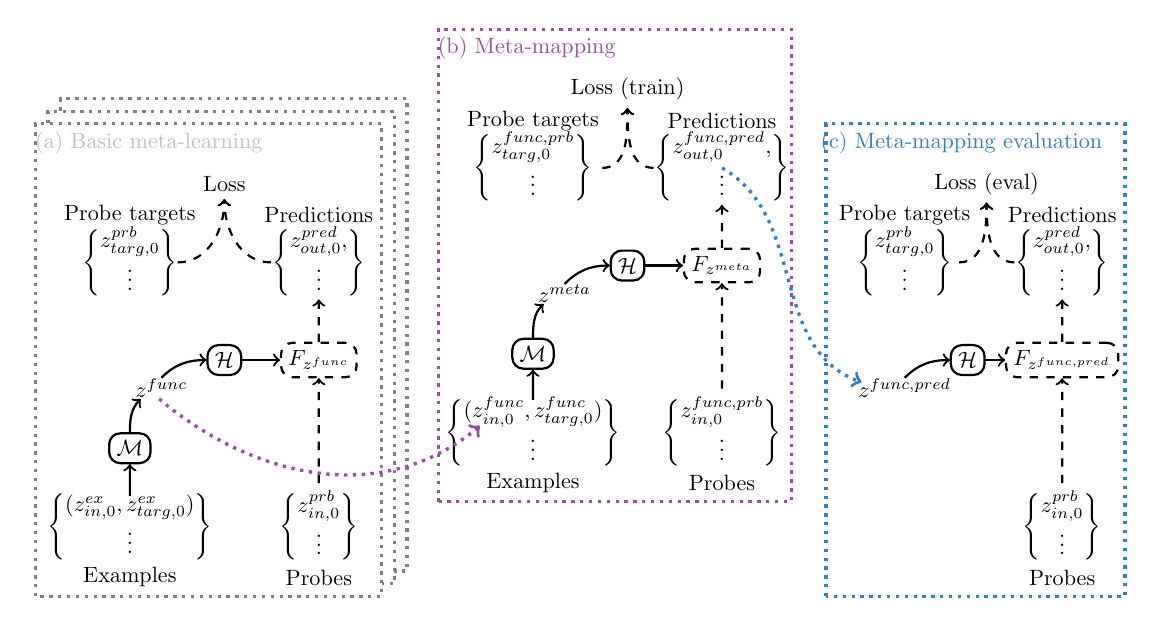
\begin{tikzpicture}[scale=0.8, every node/.style={scale=0.8}]
%% basic meta learning
\begin{scope}[shift={(0.4, 0.4)}]
\draw[boundingbox, fill=white] (-3, -4.3) rectangle (2.5, 3.2);
\end{scope}
\begin{scope}[shift={(0.2, 0.2)}]
\draw[boundingbox, fill=white] (-3, -4.3) rectangle (2.5, 3.2);
\end{scope}

\draw[boundingbox, fill=white] (-3, -4.3) rectangle (2.5, 3.2);
\node[lightgray] at (-1.2, 2.9) {(a) Basic meta-learning};
\node at (-1.5, -4) (examples) {Examples};
\node at (-1.5, -3.2) (D1) {
\(\left\{
\begin{matrix}
(z^{ex}_{in,0}, z^{ex}_{targ,0})\\
$\vdots$
\end{matrix}\right\}\)};

\node at (1.5, -4) (probes) {Probes};
\node at (1.5, -3.2) (D2) {
%\(z^{prb}_{in}\)};
\(\left\{
\begin{matrix}
z^{prb}_{in,0}\\
$\vdots$
\end{matrix}\right\}\)};

\node [block] at (-1.5, -1.95) (M) {\(\mathcal{M}\)};
\path [arrow] ([yshift=-5]D1.north) to (M);

\node at (-1, -1) (zfunc) {\(z^{func}\)};
\path [arrow, out=90, in=-135] (M.north) to ([xshift=6,yshift=3]zfunc.south west);

\node[block] at (0, -0.55) (H) {\(\mathcal{H}\)};
\path [arrow, out=45, in=180] ([yshift=-3]zfunc.north) to (H.west);

\node [block, dashed] at (1.5, -0.55) (F) {\(F_{z^{func}}\)};
\path[arrow] (H.east) to (F.west);

\path [arrow, dashed] (D2) to (F);

\node at (1.5, 1) (outputs) {
%\(z^{pred}_{out}\)};
\(\left\{
\begin{matrix}
z^{pred}_{out,0},\\
$\vdots$
\end{matrix}\right\}\)};
\node at (1.5, 1.75) (predictions) {Predictions};

\path [arrow, dashed] (F) to ([yshift=3]outputs.south);

\node at (-1.5, 1.75) (probetargs) {Probe targets};
\node at (-1.5, 1) (D2targs) {
%\(z^{prb}_{in}\)};
\(\left\{
\begin{matrix}
z^{prb}_{targ,0}\\
$\vdots$
\end{matrix}\right\}\)};

\node [align=center, text width=1.25 cm] at (0, 2.25) (dispatch) {\baselineskip=12pt Loss\par};

\path [arrow, dashed, out=180, in=-90] ([xshift=3]outputs.west) to (dispatch.south);

\path [arrow, dashed, out=0, in=-90] ([xshift=-3.5]D2targs.east) to (dispatch.south);



%% meta mapping
\begin{scope}[shift={(6.4, 1.5)}]
\draw[boundingbox, draw=bpurp, fill=white] (-3, -4.3) rectangle (2.6, 3.2);
\node[bpurp] at (-1.6, 2.9) {(b) Meta-mapping};
\node at (-1.5, -4) (metaexamples) {Examples};
\node at (-1.5, -3.2) (metaD1) {
\(\left\{
\begin{matrix}
(z^{func}_{in,0}, z^{func}_{targ,0})\\
$\vdots$
\end{matrix}\right\}\)};

\node at (1.5, -4) (metaprobes) {Probes};
\node at (1.5, -3.2) (metaD2) {
%\(z^{prb}_{in}\)};
\(\left\{
\begin{matrix}
z^{func,prb}_{in,0}\\
$\vdots$
\end{matrix}\right\}\)};

\node [block] at (-1.5, -1.95) (metaM) {\(\mathcal{M}\)};
\path [arrow] ([yshift=-5]metaD1.north) to (metaM);

\node at (-1, -1) (metazfunc) {\(z^{meta}\)};
\path [arrow, out=90, in=-135] (metaM.north) to ([xshift=6,yshift=3]metazfunc.south west);

\node[block] at (0, -0.55) (metaH) {\(\mathcal{H}\)};
\path [arrow, out=45, in=180] ([yshift=-3]metazfunc.north) to (metaH.west);

\node [block, dashed] at (1.5, -0.55) (metaF) {\(F_{z^{meta}}\)};
\path[arrow] (metaH.east) to (metaF.west);

\path [arrow, dashed] (metaD2) to (metaF);

\node at (1.5, 1) (metaoutputs) {
%\(z^{pred}_{out}\)};
\(\left\{
\begin{matrix}
z^{func,pred}_{out,0},\\
$\vdots$
\end{matrix}\right\}\)};
\node at (1.5, 1.75) (metapredictions) {Predictions};

\path [arrow, dashed] (metaF) to ([yshift=3]metaoutputs.south);

\node at (-1.5, 1.75) (metaprobetargs) {Probe targets};
\node at (-1.5, 1) (metaD2targs) {
%\(z^{prb}_{in}\)};
\(\left\{
\begin{matrix}
z^{func,prb}_{targ,0}\\
$\vdots$
\end{matrix}\right\}\)};

\node [align=center] at (0, 2.25) (metadispatch) {Loss (train)};

\path [arrow, dashed, out=180, in=-90] ([xshift=3]metaoutputs.west) to (metadispatch.south);

\path [arrow, dashed, out=0, in=-90] ([xshift=1]metaD2targs.east) to (metadispatch.south);


\end{scope}
\path [arrow, very thick, draw=bpurp, dotted, out=-40, in=-140] ([xshift=-1, yshift=3]zfunc.south) to ([xshift=19, yshift=3]metaD1.west);

%% evaluating meta mapping
\begin{scope}[shift={(11.8, 0)}]
\draw[boundingbox, draw=bblue, fill=white] (-2.25, -4.3) rectangle (2.5, 3.2);
\node[bblue] at (-0.1, 2.9) {(c) Meta-mapping evaluation};

\node at (1.5, -4) (metaevalprobes) {Probes};
\node at (1.5, -3.2) (metaevalD2) {
%\(z^{prb}_{in}\)};
\(\left\{
\begin{matrix}
z^{prb}_{in,0}\\
$\vdots$
\end{matrix}\right\}\)};

\node at (-1, -1) (metaevalzfunc) {\(z^{func,pred}\)};

\node[block] at (0, -0.55) (metaevalH) {\(\mathcal{H}\)};
\path [arrow, out=45, in=180] ([yshift=-3]metaevalzfunc.north) to (metaevalH.west);

\node [block, dashed] at (1.5, -0.55) (metaevalF) {\(F_{z^{func,pred}}\)};
\path[arrow] (metaevalH.east) to (metaevalF.west);

\path [arrow, dashed] (metaevalD2) to (metaevalF);

\node at (1.5, 1) (metaevaloutputs) {
%\(z^{pred}_{out}\)};
\(\left\{
\begin{matrix}
z^{pred}_{out,0},\\
$\vdots$
\end{matrix}\right\}\)};
\node at (1.5, 1.75) (metaevalpredictions) {Predictions};

\path [arrow, dashed] (metaevalF) to ([yshift=3]metaevaloutputs.south);

\node at (-1, 1.75) (metaevalprobetargs) {Probe targets};
\node at (-1, 1) (metaevalD2targs) {
%\(z^{prb}_{in}\)};
\(\left\{
\begin{matrix}
z^{prb}_{targ,0}\\
$\vdots$
\end{matrix}\right\}\)};

\node [align=center] at (0.3, 2.25) (metaevaldispatch) {Loss (eval)};

\path [arrow, dashed, out=180, in=-90] ([xshift=3]metaevaloutputs.west) to (metaevaldispatch.south);

\path [arrow, dashed, out=0, in=-90] ([xshift=-0.5]metaevalD2targs.east) to (metaevaldispatch.south);
\end{scope}
\path [arrow, very thick, draw=bblue, dotted, out=-30, in=160] (metaoutputs.center) to ([xshift=5, yshift=-5]metaevalzfunc.north west);
\end{tikzpicture}
\caption{The HoMM architecture allows for transformations at different levels of abstraction. (a) For basic meta-learning a dataset consisting of (input embedding, output embedding) tuples is processed by the meta-network \(\mathcal{M}\) to produce a function embedding \(z^{func}\), which is processed by the hyper network \(\mathcal{H}\) to parameterize a function \(F_{z^{func}}\), which attempts to compute the transformation on held-out probe inputs. However, our approach goes beyond basic meta-learning. The function embedding \(z^{func}\) can then be seen as a single input or output at the next level of abstraction, when the same networks \(\mathcal{M}\) and \(\mathcal{H}\) are used to transform function embeddings based on examples of a meta-mapping (b). To evaluate meta-mapping performance, a probe embedding of a held-out function is transformed by the architecture to yield a predicted embedding for the transformed task. The performance of this predicted embedding is evaluated by moving back down a level of abstraction and evaluating on the actual target task (c). Because the function embedding is predicted by a transformation rather than from examples, new tasks can be performed zero-shot. (\(M\) and \(H\) are learnable deep networks, and $F_{z}$ is a deep network parameterized by $\mathcal{H}$ conditioned on function embedding \(z\). Input and output encoders/decoders are omitted for simplicity. See the text and appendix \ref{app_model_details} for details.)} \label{architecture_inference_fig}
\end{figure}
\looseness=-1
More formally, we treat functions and data as entities of the same type. From this perspective, the data points that one function receives can themselves be functions\footnote{Indeed, any data point can be represented as a constant function that outputs the data point.}. The key insight is that then our architecture can transform data points\footnote{Where ``data'' is a quite flexible term. The approach is agnostic to whether the learning is supervised or reinforcement learning, whether inputs are images or natural language, etc.} to perform basic tasks (as is standard in machine learning), but it can also transform these task functions to adapt to new tasks. This is related to the concepts of homoiconicity, defined above, and higher-order functions. Under this perspective, basic tasks and meta-mappings from task to task are really the same type of problem. The functions at one level of abstraction (the basic tasks) become inputs and outputs for higher-level functions at the next level of abstraction (meta-mapping between tasks). \par
Specifically, we embed each input, target, or mapping into a shared representational space $Z$. This means that single data points are embedded in the same space as the representation of a function or an entire dataset. Inputs are embedded by a deep network $\mathcal{I}: \text{input} \rightarrow Z$. Model outputs are decoded from $Z$ by $\mathcal{O}: Z \rightarrow \text{output}$. Target outputs are encoded by $\mathcal{T}: \text{targets} \rightarrow Z$.\par
Given this, the task of mapping inputs to outputs can be framed as trying to find a transformation of the representational space that takes the (embedded) inputs from the training set to embeddings that will decode to the target outputs. These transformations are performed by a system with the following components (see fig. \ref{architecture_inference_fig}): $\mathcal{M}: \{(Z, Z), ...\} \rightarrow Z $ -- the meta network, which collapses a dataset of (input embedding, target embedding) pairs to produce a single function embedding. $\mathcal{H}: Z \rightarrow \text{parameters}$ -- the hyper network, which maps a function embedding to parameters. $F: Z \rightarrow Z$ -- the transformation, implemented by a deep network parameterized by $\mathcal{H}$. \par
\vspace{-0.5em}
\paragraph{Basic meta-learning:} To perform a basic task, input and target encoders ($\mathcal{I}$ and $\mathcal{T}$) are used to embed individual pairs from an example dataset \(D_1\), to form a dataset of example (input, output) tuples (fig. \ref{architecture_inference_fig}a). These examples are fed to $\mathcal{M}$, which produces a function embedding (via a deep neural network, with several layers of parallel processing across examples, followed by an element-wise max across examples, and several more layers). This function embedding is mapped through the hyper network $\mathcal{H}$ to parameterize $F$, and then $F$ is used to process a dataset of embedded probe inputs, and $\mathcal{O}$ to map the resultant embeddings to outputs. This system can be trained end-to-end on target outputs for the probes. Having two distinct datasets forces generalization at the meta-learning level, see appendix \ref{app_clarifying_holdouts}. See appendix \ref{app_model_details} for detailed architecture, and hyper-parameters. \par 
More explicitly, suppose we have a dataset of example input, target pairs ($D_1 = \{(x_0, y_0), ...\}$), and some input $x$ from a probe dataset $D_2$. The system would predict a corresponding output $\hat{y}$ as: 
\[\hat{y} = \mathcal{O}\left(F_{z^{func}}\left(\mathcal{I} \left(x\right)\right) \right)\]
where $F_{z^{func}}$ is the meta-learner's representation for the function underlying the examples in $D_1$:
\[F_{z^{func}} \text{ is parameterized by } \mathcal{H}\left(z^{func}\right), \text{ where } z^{func} = \mathcal{M}\left( \left\{\left(\mathcal{I}\left(x_0\right), \mathcal{T}\left(y_0\right) \right), ... \right\}\right)\]
Then, given some loss function $\mathfrak{L}(y, \hat{y})$ defined on a single target output $y$ and an actual model output $\hat{y}$, we define our total loss computed on the probe dataset $D_2$ as: 
\[\mathbb{E}_{(x, y)\in {D}_2} \left[ \mathfrak{L}\left(y, \mathcal{O}\left(F_{D_1}\left(\mathcal{I} \left(x\right)\right) \right)\right)\right]\]
The system can then be trained end-to-end on this loss to adjust the weights of \(\mathcal{T,H,M,O}\), and \(\mathcal{I}\).
\vspace{-0.25em}
\paragraph{Meta-mapping:} The fundamental insight of our paper is to show how basic tasks and meta-mappings can be treated homogenously, by allowing the network to transform its task representations like data (see fig. \ref{architecture_inference_fig}b,c). From the perspective of our architecture, learning a meta-mapping between tasks is exactly analogous to learning a basic task. Anything that is embedded in $Z$ can be transformed using the same system. Because tasks are embedded in $Z$ for basic meta-learning, this allows for meta-mappings using exactly the same $\mathcal{M}$ and $\mathcal{H}$ that we use for basic tasks. Just as we would take a set of paired embeddings of data points for a basic task, and use them to compute a function embedding for that task, we can take a set of paired function embeddings, and use them to create an embedding for the meta-mapping. We can then use this meta-mapping embedding to transform another task. We can thus behave zero-shot on a novel task based on its relationship to a prior task. \par
For example, suppose we have an embedding $z_{game1} \in Z$ for the task of playing some game, and we want to switch to trying to lose this game. We can generate a meta-mapping embedding $z_{\text{meta}} \in Z$ from examples of embeddings generated by the system when it is trying to win and lose various games: $z_{\text{meta}} = \mathcal{M}\left( \left\{\left((z_{game2},z_{game2,lose}\right), ... \right\}\right)$. We can generate a new task embedding $\hat{z}_{game1,lose} \in Z$:  
\[\hat{z}_{game1,lose} = F_{z_{\text{meta}}}(z_{game1}) \qquad \text{where } F_{z_{\text{meta}}} \text{ is parameterized by } \mathcal{H}\left(z_{\text{meta}}\right)\]
\looseness=-1
This $\hat{z}_{games1,lose}$ can be interpreted as the system's guess at a losing strategy for game 1. To train a meta-mapping, we minimize the $\ell_2$ loss in the latent space betwen this guessed embedding and the embedding of the target task\footnote{The gradients do not update the example function embeddings, only the weights of \(\mathcal{M}\) and \(\mathcal{H}\), due to memory contraints. Allowing this might be useful in more complex applications.}. Whether or not we have such a target embedding, we can evaluate how well the system loses with this $\hat{z}_{game1,lose}$ strategy, by stepping back down a level of abstraction and actually having it play the game via this embedding (fig. \ref{architecture_inference_fig}c). This is how we evaluate meta-mapping performance -- evaluating the loss of transformed task embeddings on the respective target tasks. \par
Alternatively, we could map from language to a meta-mapping embedding, rather than inducing it from examples of the meta-mapping. This corresponds to the human ability to change behavior in response to instructions. The key feature of our architecture -- the fact that tasks, data, and language are all embedded in a shared space -- allows for substantial flexibility within a unified framework. Furthermore, our approach is parsimonious. Because it uses the same meta-learner for both basic tasks and meta-mappings, this increased flexibility does not require any added parameters.\footnote{At least in principle, in practice of course increasing network size might be more beneficial for HoMM architectures performing meta-mappings as well as basic tasks, compared to those performing only basic tasks.}  

%\subsection{Boolean functions}
%As a proof of concept, we first evaluated the system on a simple task of computing boolean functions on boolean inputs. Specifically, we can imagine mapping from binary-valued input vectors to a single binary output representing the evaluation of some logical proposition on the input. We train the system to figure out how to compute the predicate from seeing a subset of the (input, output) pairs. \par   
%We can then train the system to do various meta-mappings, for example identifying certain types of functions (like XOR) or negating predicates. \par
%
\section{Learning multivariate polynomials} \label{sec_poly}
\begin{figure}[t]
\centering
\begin{subfigure}[t]{0.5\textwidth}
\includegraphics[width=\textwidth]{2-HoMM/figures/poly/basic_results.png}
\caption{The polynomials domain, section \ref{sec_poly}.}
\label{poly_basic_results}
\end{subfigure}%
\begin{subfigure}[t]{0.5\textwidth}
\includegraphics[width=\textwidth]{2-HoMM/figures/basic_meta_learning.png}
\caption{The cards domain, section \ref{sec_cards}.}
\label{cards_basic_results}
\end{subfigure}%
\caption{The HoMM system succeeds at basic meta-learning, which is a necessary prerequisite for meta-mappings. (\subref{poly_basic_results}) The polynomials domain, section \ref{sec_poly}. The system successfully generalizes to held out polynomials. The solid line indicates optimal performance; the dashed line indicates untrained model performance. (\subref{cards_basic_results}) The card games domain, section \ref{sec_cards}. The system successfully generalizes to held out games, both when trained on a random sample of half the tasks, or when a targeted subset is held out. The gray dashed line indicates chance performance, while the solid lines are optimal performance. The orange dashed lines shows performance on held-out tasks of playing the strategy from the most correlated trained task. The fact that the system generally exceeds this difficult baseline shows a deeper form of generalization than just memorizing strategies and picking the closest. Error-bars throughout are bootstrap 95\%-confidence intervals, numerical values for plots can be found in appendix \ref{app_numerical_results}.}
\end{figure}

\begin{figure}[t]
\centering
\begin{subfigure}{0.5\textwidth}
\includegraphics[width=\textwidth]{2-HoMM/figures/poly/meta_results.png}
\caption{The polynomials domain, section \ref{sec_poly}.}
\label{poly_meta_map_results_examples}
\end{subfigure}%
\begin{subfigure}{0.5\textwidth}
\includegraphics[width=\textwidth]{2-HoMM/figures/meta_mapping.png}
\caption{The cards domain, section \ref{sec_cards}.}
\label{cards_meta_map_results_examples}
\end{subfigure}%
\caption{The HoMM architecture performs well at meta-mappings. (\subref{poly_meta_map_results_examples}) The system generalizes to apply learned meta-mappings to new polynomials, and even to apply unseen meta-mappings. The plots show the loss produced when evaluating the mapped embedding on the target task. For example, if the initial polynomial is $p(x) = x + 1$, and the meta-task is ``square,'' the loss would be evaluated by transforming the embedding of $p(x)$ and evaluating how well the mapped embedding regresses on to $p(x)^2 = x^2 + 2x + 1$. The results show that the system succeeds at applying meta-mappings it is trained on to held-out polynomials, as well as applying held-out meta-mappings to either trained or held-out polynomials. The solid line indicates optimal performance; the dashed line is untrained model performance.
(\subref{cards_meta_map_results_examples}) The system generalizes to meta-mapping new tasks in the cards domain. The system is trained to do the meta-mappings shown here on a subset of its basic tasks, and is able to generalize these mappings to perform novel tasks zero-shot. For example, for the ``losers'' mapping, the sytem is trained to map games to their losers variants. When given a held-out game, it is able to apply the mapping to guess how to play the losing variation. This plot shows the reward produced by taking the mapped embedding and playing the targeted game. The gray dashed line indicates random performance, while the colored dashed lines indicate performance if the system did not alter its behavior in response to the meta-mapping. The system generally exceeds these baselines, although the switch-suits baseline is more difficult with the targeted holdout. 
Error-bars are bootstrap 95\%-CIs.} 
\label{meta_map_results}
\end{figure}

As a proof of concept, we first evaluated the system on the task of learning polynomials of degree $\leq 2$ in 4 variables (i.e. the task was to regress functions of the form $p: \mathbb{R}^4 \rightarrow \mathbb{R}$ where $p \in \mathcal{P}_2 \left(\mathbb{R}\right)$, though the model was given no prior inductive bias toward polynomial forms). For example, if $p(w,x,y,z) = x$, the model might see examples like $(-1,1,1,1; 1)$ and $(0.7, 2.1, 1.3, -4; 2.1)$, and be evaluated on its output for points like $(-1, -1.3, 0.5, 0.3)$. This yields an infinite family of base-level tasks (the vector space of all such polynomials), as well as many families of meta-mappings over tasks (for example, multiplying polynomials by a constant, squaring them, or permuting their input variables). This allows us to not only examine the ability of the system to learn to learn polynomials from data, but also to adapt its learned representations in accordance with these meta-tasks. Details of the architecture and training can be found in appendix \ref{app_detailed_methods}.\par
\vspace{-0.7em}
\paragraph{Basic meta-learning:} First, we show that the system is able to achieve the basic goal of learning a held-out polynomial from a few data points in fig. \ref{poly_basic_results} (with good sample-efficiency, see supp. fig. \ref{supp_poly_sweep_results}). \par 
\vspace{-0.7em}
\paragraph{Meta-mapping (task $\rightarrow$ task):} Furthermore, the system is able to perform meta-mappings over polynomials in order to flexibly reconfigure its behavior (fig. \ref{poly_meta_map_results_examples}). We train the system to perform a variety of mappings, for example switch the first two inputs of the polynomial, add 3 to the polynomial, or square the polynomial. We then test its ability to generalize to held-out mappings from examples, for example a held-out input permutation, or an unseen additive shift. The system is both able to apply learned meta-mappings to held-out polynomials, and to apply held-out meta-mappings it has not been trained on, simply by seeing examples of the mapping. \par 

\section{A stochastic learning setting: simple card games}\label{sec_cards}
%\vspace{-0.5em} % section
We next explored the setting of simple card games, where the agent is dealt a hand and must bet. There are three possible bets (including ``don't bet''), and depending on the opponent's hand the agent either wins or loses the amount bet. This task doesn't require long term planning, but does incorporate some aspects of reinforcement learning, namely stochastic feedback on only the action chosen. We considered five games that are simplified analogs of various real card games (see Appendix \ref{meth_data_cards}). We also considered several binary options that could be applied to the games, including trying to lose instead of trying to win, or switching which suit was more valuable. These are challenging manipulations, for instance trying to lose requires completely inverting a learned $Q$-function. \par
%% Can cut The hand is explicitly ..., maybe some other stuff
In order to adapt the HoMM architecture, we made a very simple change. Instead of providing the system with (input, target) tuples to embed, we provided it with (state, action, reward) tuples, and trained it to predict rewards for each bet in each state. (A full RL framework is not strictly necessary here because there is no temporal aspect to the tasks; however, because the outcome is only observed for the action you take, it is not a standard supervised task.) The hand is explicitly provided to the network for each example, but which game is being played is implicitly captured in the training examples, without any explicit cues. That is, the system must learn to play directly from seeing a set of (state, action, reward) tuples which implicitly capture the structure and stochasticity of the game. We also trained the system to make meta-mappings, for example switching from trying to win a game to trying to lose. Details of the architecture and training can be found in appendix \ref{app_detailed_methods}. \par
%\vspace{-0.7em}
\paragraph{Basic meta-learning:} First, we show that the system is able to play a held-out game from examples in fig. \ref{cards_basic_results}. We compare two different hold-out sets: 1) train on half the tasks at random, or 2) specifically hold out all the ``losers'' variations of the ``straight flush'' game. In either of these cases, the meta-learning system achieves well above chance performance (0) at the held out tasks, although it is slightly worse at generalizing to the targeted hold out, despite having more training tasks in that case. Note that the sample complexity in terms of number of trained tasks is not that high, even training on 20 randomly selected tasks leads to good generalization to the held-out tasks. Furthermore, the task embeddings generated by the system are semantically organized, see appendix \ref{app_cards_tsne}. \par
%\vspace{-0.7em}
\paragraph{Meta-mapping (task $\rightarrow$ task):} Furthermore, the system is able to perform meta-mappings (mappings over tasks) in order to flexibly reconfigure its behavior. For example, if the system is trained to map games to their losers variations, it can generalize this mapping to a game it has not been trained to map, even if the source or target of that mapping is held out from training. In fig. \ref{cards_meta_map_results_examples} we demonstrate this by taking the mapped embedding and evaluating the reward received by playing the targeted game with it. This task is more difficult than simply learning to play a held out game from examples, because the system will actually receive no examples of the target game (when it is held out). Furthermore, in the case of the losers mapping, leaving the strategy unchanged would produce a large negative reward, and chance performance would produce 0 reward, so the results are quite good. \par
%\vspace{-0.5em}
\section{An extension via language}
%\vspace{-0.5em} % section
\begin{figure}
\centering
\begin{subfigure}{0.5\textwidth}
\includegraphics[width=\textwidth]{2-HoMM/figures/poly/language_meta_results.png}
\caption{The polynomials domain.}
\label{poly_meta_map_results_language}
\end{subfigure}%
\begin{subfigure}{0.5\textwidth}
\includegraphics[width=\textwidth]{2-HoMM/figures/language_meta_mapping.png}
\caption{The cards domain.}
\label{cards_meta_map_results_language}
\end{subfigure}
\caption{The HoMM system can perform meta-mappings from language cues rather than meta-mapping examples. Compare to fig. \ref{meta_map_results}, which shows the same results when using examples instead of language. (\subref{poly_meta_map_results_language}) In the polynomials domain, language cues still lead to good performance, even on held-out tasks or held-out meta-mappings, although examples perform slightly better (fig. \ref{poly_meta_map_results_examples}). (\subref{cards_meta_map_results_language}) Similarly, in the cards domain, language cues perform well. Error-bars are bootstrap 95\%-CIs.}
\label{language_meta_map_results}
\end{figure}
Language is fundamental to human flexibility. Often the examples of the meta-mapping are implicit in prior knowledge about the world that is cued by language. For example, ``try to lose at go'' does not give explicit examples of the ``lose'' meta-mapping, but rather relies on prior knowledge of what losing means. This is a much more efficient way to cue a known meta-mapping. In order to replicate this, we trained the HoMM system with both meta-mappings based on examples, and meta-mappings based on language. In the language-based meta-mappings, a language input identifying the meta-mapping (but not the basic task to apply it to) is encoded by a language encoder, and then provided as the input to $\mathcal{H}$ (instead of an output from $\mathcal{M}$). The meta-mapping then proceeds as normal --- $\mathcal{H}$ parameterizes $F$, which is used to transform the embedding of the input task to produce an embedding for the target. \par
This language-cued meta-mapping approach also yields good performance (fig. \ref{language_meta_map_results}). However, examples of the meta-mapping are slightly better, especially for meta-mappings not seen during training, presumably because examples provide a richer description. In Appendix \ref{app_why_meta_mapping} we show that using language to specify a meta-mapping performs better than using language to directly specify the target task, presumably by leveraging the richer task representation of the task embedding. \par

%\vspace{-0.5em}
\section{Discussion} \label{sec_discussion}
%\vspace{-0.5em} % section
\paragraph{Related work:} Our work is an extrapolation from the rapidly-growing literature on meta-learning \citep[e.g.][]{Vinyals2016, Santoro2016, Finn2017a, Finn2018, Stadie2018, Botvinick2019}. It is also related to the literature on continual learning, or more generally tools for avoiding catastrophic interference based on changes to the architecture \citep[e.g.][]{Fernando2017, Rusu2016}, loss \citep[e.g.][]{Kirkpatrick2016, Zenke2017, Aljundi2019}, or external memory \citep[e.g.][]{Sprechmann2018}. We also connect to a different perspective on continual learning in appendix \ref{app_continual}. Recent work has also begun to blur the separation between these approaches, for example by meta-learning in an online setting \citep{Finn2019}. Our work is specifically inspired by the algorithms that attempt to have the system learn to adapt to a new task via activations rather than weight updates, either from examples \citep[e.g.][]{Wang2016a, Duan2016}, or a task input \citep[e.g.][]{Borsa2019}. \par
Our architecture builds directly off of prior work on HyperNetworks \citep{Ha2016} -- networks which parameterize other networks -- and other recent applications thereof, such as guessing parameters for a model to accelerate model search \citep[e.g.][]{Brock2018a, Zhang2019}, and meta-learning \citep[e.g.]{Li2019a, Rusu2019}. Our work is also related to the longer history of work on different time-scales of weight adaptation \citep{Hinton1982, Kumaran2016} that has more recently been applied to meta-learning contexts \citep[e.g.][]{Ba2016, Munkhdalai2017, Garnelo2018} and continual learning \citep[e.g.]{Hu2019}. It is more abstractly related to work on learning to propose architectures \citep[e.g.][]{Zoph2016, Cao2019}, and to models that learn to select and compose skills to apply to new tasks \citep[e.g.][]{Andreas, Andreas2016, Tessler2016, Reed2015, Chang2019a}. In particular, some of the work in domains like visual question answering has explicitly explored the idea of building a classifier conditioned on a question \citep{Andreas, Andreasa}, which is related to one of the possible computational paths through our architecture. Work in model-based reinforcement learning has also partly addressed how to transfer knowledge between different reward functions \citep[e.g.][]{Laroche2017}; our approach is more general. Indeed, our insights could be combined with model-based approaches, for example our approach could be used to adapt a task embedding, which would then be used by a learned planning model.\par 
There has also been other recent interest in task (or function) embeddings. Achille et al. \citep{Achille2019} recently proposed computing embeddings for visual tasks from the Fisher information of the parameters in a model partly tuned on the task. They show that this captures some interesting properties of the tasks, including some types of semantic relationships, and can help identify models that can perform well on a task. Rusu and colleagues recently suggested a similar meta-learning framework where latent codes are computed for a task which can be decoded to a distribution over parameters \citep{Rusu2019}. Other recent work has tried to learn representations for skills \citep[e.g.][]{Eysenbach2019} or tasks \citep[e.g.]{Hsu2019} for exploration and representation learning. Our perspective can be seen as a generalization of these that allows for remapping of behavior via meta-tasks. To the best of our knowledge none of the prior work has explored zero-shot performance of a task via meta-mappings. \par
% \vspace{-1em}
\paragraph{Future Directions:} We think that the general perspective of considering meta-mappings will yield many fruitful future directions. We hope that our work will inspire more exploration of behavioral adaptation, in areas beyond the simple domains we considered here. To this end, we suggest the creation of meta-learning datasets which include information not only about tasks, but about the relationships between them. For example, reinforcement learning tasks which involve executing instructions \citep[e.g.][]{Hermann2017, Co-Reyes2019} can be usefully interpreted from this perspective. Furthermore, we think our work provides a novel perspective on the types of flexibility that human intelligence exhibits, and thus hope that it may have implications for cognitive science. \par 
We do not necessarily believe that the particular architecture we have suggested is the best architecture for addressing these problems, although it has a number of desirable characteristics. However, the modularization of the architecture makes it easy to modify. (We compare some variations in appendix \ref{app_lesion_results}.) For example, although we only considered task networks $F$ that are feed-forward and of a fixed depth, this could be replaced with a recurrent architecture to allow more adaptive computation, or even a more complex architecture \citep[e.g.][]{Reed2015, Graves2016}. Our work also opens the possibility of doing unsupervised learning over function representations for further learning, which relates to long-standing ideas in cognitive science about how humans represent knowledge \citep{Clark1993}. \par 
%\vspace{-1em}
%\paragraph{Conclusions:}
\section{Conclusions}
%\vspace{-0.5em} % section
\looseness=-1
We've highlighted a new type of flexibility in the form of meta-mapping between tasks. Meta-mapping can produce zero-shot performance on novel tasks, based on their relationship to old tasks. This is a key aspect of human flexibility, but is lacking from most contemporary deep-learning models. Achieving this flexibility requires representing tasks in a transformable way. To address this, our Homoiconic Meta-Mapping (HoMM) approach explicitly represents tasks by function embeddings, and derives the computation from these embeddings via a HyperNetwork. This allows for our key insight: by embedding tasks and individual data points in a shared latent space, the same meta-learning architecture can be used both to transform data for basic tasks, and to transform task embeddings to adapt to task variations. This approach is parsiomious, because it uses the same networks for basic- and meta-mappings. Perhaps because of this, the requisite meta-task sample complexity is small; we showed generalization to unseen meta-mappings after training on only 20 meta-mappings. That is, we are able to achieve zero-shot performance on a novel task based on a held-out relationship between tasks. This is a step closer to human-level flexibility.\par
We see our proposal as a logical progression from the fundamental idea of meta-learning -- that there is a continuum between data and tasks. This naturally leads to the idea of manipulating task representations just like we manipulate data. We've shown that this approach yields considerable flexibility, most importantly the meta-mapping ability to adapt zero-shot to a new task. We hope that these results will lead to the development of more powerful and flexible deep-learning models. \par
\subsubsection*{Acknowledgements}
We would like to acknowledge Noah Goodman, Surya Ganguli, Katherine Hermann, Erin Bennett, and Arianna Yuan for stimulating questions and suggestions on this project.


\chapter{Comparing to human adaptation} \label{chapter:human}

In the previous chapter I proposed a framework for modeling human adaptation to new tasks, based on relationships between tasks. To evaluate the quality of the framework, it is necessary to compare its adaptation to human adaptation. \par
It is worth stopping for a moment to consider how flexible humans actually are. We certainly experience short-term interference from switching tasks or goals \citep{Rogers1995}, or when we try to override a habitual response \citep{Stroop1935, MacLeod1991}. Over longer periods of time, our adaptation might be a response to learning in the new situation, rather than the type of zero-shot flexbiility that HoMM is intended to model. How flexibly are humans able to adapt to task changes in a short amount of time? \par
Unfortunately a complete evaluation of human flexibility is a large research program. In this chapter we present an evaluation of human adaptation in one setting, inspired by a motivating example used in the previous chapters. We taught participants a simplified poker-like card game, and evaluated how well they were able to switch to losing the game, after practicing trying to win. This is a difficult form of adaptation, which requires completely reversing a value function, and has been highlighted as a challenge for deep learning \citep{Lake2016}.\par
We compared human performance on the game to both a HoMM model and a task-description-based language-generalization model. We trained both models on variations of 5 card-game tasks, including losing variations of 4 of these, but crucially holding out all losing variations of the task that the human subjects played. We then evaluated the ability of the models to adapt to the losing variation zero-shot, just as we had evaluated the humans. In the HoMM model, this adaptation was based on applying a ``switch-to-losing'' meta-mapping to the learned variation of the game, whereas in the language-generalization model it was based on a novel instruction to lose the game that was systematically related to the training instructions for losing other games.\par 

\section{Experimental design}
The human experiment was conducted on Amazon Mechanical Turk. 
We tried to design the game that participants played to make it easy for them to learn, without relying on their prior knowledge of card games. The game was a simplified variation of poker. The participants were dealt hands which consisted of two cards, each with a number (rank) between 1 and 4, and a color (suit) of red or black. The participants played against a computer opponent that was dealt a similar hand. The hands were ranked such that straight flushes (adjacent cards in the same suit) beat adjacent cards in a different suit, which beat non-adjacent cards (including pairs). Ties were broken by the highest card, or by suit if both cards were tied. \par
\begin{figure}
\centering
\begin{subfigure}[b]{0.5\textwidth}
\includegraphics[width=\textwidth]{3-human-adaptation/figures/pre_bet_screenshot.png}
\caption{Before betting.}
\end{subfigure}%
\begin{subfigure}[b]{0.5\textwidth}
\includegraphics[width=\textwidth]{3-human-adaptation/figures/post_bet_screenshot.png}
\caption{Feedback.} \label{fig:human_betting_trial_feedback}
\end{subfigure}%
\caption{The card game experiment trials, as seen by participants.} \label{fig:human_betting_trial}
\end{figure}
On each trial, participants were dealt a hand and asked to make a bet of 0, 5, or 10 cents (see Fig. \ref{fig:human_betting_trial}). If their hand beat the opponent's hand, they won the bet amount. If their hand lost, they lost it. If the hands were tied, they neither won nor lost money. \par
The experiment had several phases. First, participants were instructed in the rules and payment scheme for the experiment. Next, they were instructed on the rules of the game. After this, they were tested with four hand-comparison trials intended to probe their understanding of each of the rules of the game. If they failed more than one of these trials, they were not allowed to continue with the experiment. \par
Following this understanding check, participants played a block of 32 hands (sampled to have a diversity of expected values), where they saw the results of their play (as in Fig. \ref{fig:human_betting_trial_feedback}). After this block, they played a similar block of 24 trials where they did not see the results of their play. The results were replaced with a brief grayed-out screen, and participants were payed the net expected value of their actions over the block (rounded to the nearest 10). This provides an evaluation phase with relatively less potential for learning. \par
Finally, participants were told that we wanted them to try to lose for the remaining trials, and that ``for the remainder of the experiment, if you bet and lose, you'll gain the amount you bet, and if you bet and win, you'll lose the amount you bet.'' They were then given an attention check to evaluate whether they had understood this instruction. Subjects who failed this attention check were excluded from the analysis. They then played another block of 24 trials where they were rewarded for losing instead of winning (i.e. the expected returns were reversed). As in the previous block, they did not see the results of their actions. They were finally asked a few demographic questions. See Appendix \ref{appendix:human} for detailed instructions \& methods.\par
Our main target comparison was performance in the two blocks without feedback -- were participants able to switch their behavior to lose at the game as well as they won at it?\par

\subsection{HoMM model}

To compare to the human participants, we wanted to evaluate the HoMM model's ability to switch to losing based on a ``try-to-lose'' meta-mapping. To do so, we needed other games (with winning and losing variations) to use as training examples of the meta-mapping. We therefore created 4 other card games, based on simplifications of other existing games, like blackjack or matching cards. We created variations of these games that switched whether suit or rank was the most important attribute, and which suit was most valuable. We created losing variations of each of these. In total, there are 5 card games \(\times\) 3 binary attributes \(= 40\) basic tasks. See Appendix \ref{app:human:model_details} for full descriptions of all the games and variations.\par

We trained the model on 36 of these games, but held out the losing variations of all versions of the game that the human subjects played. We trained the model on three meta-mappings, corresponding to toggling the three binary game attributes. We also trained the model to classify the basic game types (one vs. all) and each of the attributes. We then evaluated the ability of the model to adapt to the losing variation zero-shot, just as the humans did. This adaptation was based on instantiating the ``switch-to-losing'' meta-mapping with the 32 available examples, and applying it to the 4 other training tasks. We used the three other held-out variations of the game as a validation set to pick an optimal-stopping point for evaluating the model on the remaining hold-out (the game that the humans played). \par

In order to perform the basic tasks with the HoMM model, we had to make one minor alteration. Because in this task the model (or participant) only receives feedback on the action taken, this is not a simple regression problem with inputs and targets. It is more similar to a reinforcement learning setting, where the model takes actions and may or may not receive rewards in response (although there is no temporal component in our simplified tasks). We thus altered the way a task representation is constructed from examples in the model. Instead of using a dataset of (input, target) tuples, we used a dataset of (input, (action, reward)) tuples, where the action and reward were processed together to form a single embedding.\footnote{Note that this requires some slight abuse of the notion that the basic tasks and the meta-mappings are precisely analogous, see Section \ref{section:extending:RL:model} for some discussion.} The model was then trained with a masked loss, such that it only updated its predictions for actions it actually took, rather than other possibilities. (See Appendix \ref{app:human:model_details} for further details of the training.) \par

\subsection{Language model}

We also compared to a language-generalization baseline. As a reminder, this is an alternative approach to zero-shot task performance, where the model simply receives a natural language description of the task. The task descriptions were sequences of the form:\verb|[``game'', <game_type>,| \verb|``losers'', <losers-value>, [other attributes]]|, encoded by a 2-layer LSTM network. Similar approaches have yielded good zero-shot generalization in some domains \citep[e.g.][]{Hermann2017}. The language model was trained on the same set of tasks as the HoMM model, and was optimally stopped by using the same validation set. Aside from the construction of the task representation, the remainder of the architecture was identical to HoMM. We also compared to a simpler language architecture, more similar to those used in prior work, with similar results, see Supp. Fig. \ref{supp_fig:human:lang_tcnh}. (Again, see Appendix \ref{app:human:model_details} for further architectural details.)


\section{Human performance}
First, how well were participants able to learn the game? Participants' performance is reasonable (mean performance 64\% of optimal, bootstrap 95\%-CI \([0.57, 0.70]\)). However, they are far from optimal, and there is substantial individual variability (Fig. \ref{fig:human_cards_basic_results}). In particular, participants are sometimes making intermediate bets, which an optimal agent would never do. Furthermore, the thresholds where each subject crosses a betting probability of 0.5 are variable, some subjects are substantially over- or under-conservative. However, performance is actually more optimal than some basic statistics might suggest, see Appendix \ref{appendix:human:suboptimality}. \par 
After being asked to lose, participants also performed above chance, but far from optimally (Fig. \ref{fig:human_cards_losing_results}). So how well were they able to adapt? 

\begin{figure}
\centering
\begin{subfigure}[t]{0.5\textwidth}
\includegraphics[width=\textwidth]{3-human-adaptation/figures/testing_basic_bet_densities.png}
\caption{Bet density by expected value.}
\end{subfigure}%
\begin{subfigure}[t]{0.5\textwidth}
\includegraphics[width=\textwidth]{3-human-adaptation/figures/testing_basic_subject_response_fits.png}
\caption{Probability of non-zero bet by expected value. The red dashed line is the optimal threshold, the grey curves are the individual subject fits.}
\end{subfigure}%
\caption[Human performance on the card game task, basic game evaluation block.]{Human performance on the card game task, basic game evaluation block. While participants are performing well above chance, they are far from optimal. They make intermediate value bets, and do not switch optimally between betting and not betting. There is also substantial inter-subject variability.} \label{fig:human_cards_basic_results}
\end{figure}
\begin{figure}
\centering
\begin{subfigure}[t]{0.5\textwidth}
\includegraphics[width=\textwidth]{3-human-adaptation/figures/testing_losing_bet_densities.png}
\caption{Bet density by expected value.}
\end{subfigure}%
\begin{subfigure}[t]{0.5\textwidth}
\includegraphics[width=\textwidth]{3-human-adaptation/figures/testing_losing_subject_response_fits.png}
\caption{Probability of non-zero bet by expected value. The red dashed line is the optimal threshold, the grey curves are the individual subject fits.}
\end{subfigure}%
\caption[Human performance on the card game task, losing evaluation block.]{Human performance on the card game task, losing evaluation block. There is again substantial inter-subject variability.} \label{fig:human_cards_losing_results}
\end{figure}


\section{Adaptation in humans and HoMM}
Human adaptation was quite good, in the sense that, on average, performance was almost identically preserved (losing phase mean performance 64\%, bootstrap 95\%-CI \([0.55, 0.72]\)), see Fig. \ref{fig:human_cards_adaptation_results}. However, this average masks substantial individual variability. Because the figure plots \emph{expected} earnings, and hand values were closely matched, almost all the change from one phase to the next is due to either stochasticity in the participants policies, or non-standard adaptation. (We cannot call this non-standard adaptation sub-optimal, since it sometimes results in \emph{improved} performance on the adapted task.) It would be interesting to explore in detail what factors underlie this variability, but here we focus on the comparison to the HoMM model and language-generalization model. \par  
\begin{figure}
\centering
\includegraphics[width=0.8\textwidth]{3-human-adaptation/figures/human_adaptation.png}
\caption[Human adaptation in the cards experiment.]{Human adaptation in the cards experiment: the change in performance from the winning evaluation block to the losing evaluation block. Larger lines are the average, smaller are individual subjects. While there is substantial individual variability, average performance is preserved.} \label{fig:human_cards_adaptation_results}
\end{figure}

\begin{figure}
\centering
\includegraphics[width=0.8\textwidth]{3-human-adaptation/figures/human_adaptation_vs_HoMM.png}
\caption{Comparing human adaptation to the HoMM and language models.}\label{fig:human_cards_homm_results}
\end{figure}

\begin{figure}
\centering
\includegraphics[width=0.8\textwidth]{3-human-adaptation/figures/change_scores.png}
\caption[Comparing adaptation change scores between the humans and models.]{Comparing adaptation change scores (as \% of score on prior task) between humans and the models. While the HoMM model is slightly sub-optimal, it is not significantly different than humans. By contrast, the language-based model is near chance on the held-out tasks.} \label{fig:human_cards_homm_change_scores}
\end{figure}
In Fig. \ref{fig:human_cards_homm_results} we plot the adaptation of the models against the human results. Both models are performing near-optimally on the training tasks (see Supp. Fig. \ref{supp_fig:human:cards_basic_meta_learning} for evidence that HoMM is generalizing well at the basic meta-learning level), but of course they have much more experience with these tasks than the humans do. However, the performance of the models on the novel tasks is substantially different. Both models are worse at the losing versions of the tasks than the trained versions, but the HoMM model is still performing quite well (mean 85\%, 95\%-CI \([79, 90]\)), while the language-based model is degrading to near chance performance (mean performance on losing variation 2\%, bootstrap 95\%-CI \([-12, 16]\)).\footnote{As noted above, results are similar for the language model with a simpler task-concatenated architecture (Supp. Fig. \ref{supp_fig:human:lang_tcnh}).} \par
In order to make a more fair comparison between the human subjects and the models, in Fig. \ref{fig:human_cards_homm_change_scores} we plot performance on the losing task, as a percentage of performance on the winning tasks. Note, however, that this metric is biased against the models, because of the ceiling effect -- their scores on the adapted tasks cannot be higher than their optimal scores on the original tasks, whereas the humans are only preserving their performance on average because many of them are performing substantially better on the adapted tasks (for unclear reasons). While HoMM is adapting slightly sub-optimally, the difference between it and the human subjects is not statistically significant, either by a \(t\)-test (\(t(18.54) = -1.80\), \(p = 0.09\)), or a permutation test (\(p > 0.05\)). However, HoMM is significantly better than the language-based approach, either by a   \(t\)-test (\(t(5.37) = 9.33\), \(p < 0.001\)), or a permutation test (\(p < 0.005\)). \par

\section{Discussion}

In this chapter, I have compared the ability of humans, the HoMM model, and a language baseline to adapt to losing a simple card game. The HoMM model was trained only on variations of 4 simple card games; the human participants have likely experienced a much greater variety of games over their lifetimes. Despite this, the HoMM model was able to adapt well. The human subjects also seemed to be adapting well on average, although there was substantial variability between subjects. The model appears to be adapting slightly worse than the subjects (although the difference is not statistically significant), but without giving the model an equivalent amount of experience with games as varied as those the humans have played, it's difficult to draw a strong conlusion from these results. \par
Instead, I interpret the comparison to humans and the language model as suggesting that mechanisms like meta-mapping may offer a useful model of human adaptation. In particular, the alternative approach of generalizing based on language did not perform nearly as well, although it suffers from the same objection that it does not have the degree of language experience that humans have. Ultimately, multiple mechanisms likely play a role in explaining adaptation in different people. Meta-mapping may be one important piece of the puzzle, but I do not want to imply that it is the only one. \par 
It's intriguing to note that, while in this setting the language model degraded to near-chance performance on the adapted tasks, this is still much better than if it had failed to adapt at all. It's unclear whether this chance behavior is due to the model behaving systematically in some way that is not correlated with optimal behavior, or whether this performance is actually just random. Investigating this could provide interesting insight into the generalization of these models. \par
In summary, these results offer some insight into the adaptation capabilities of HoMM relative to humans and the language model, and suggest that meta-mapping may be a promising approach for modeling human adaptation. However, the limited number of tasks each model experienced, as well as the limited complexity of the tasks themselves, also limit the breadth of conclusions that can be drawn from the experiments in this chapter. In the next chapter, I apply the model to more complex tasks in RL and vision, that provide more challenging tests of adaptation, and support the idea that meta-mapping could be a broadly useful framework for deep learning models of cognition. \par  

\chapter{Extending meta-mapping to more complex tasks} \label{chapter:extending}
In the previous chapters we have demonstrated the succes of meta-mapping in two simple domains. While these have allowed us to demonstrate the efficacy of the approach relative to other baselines, and compare its adaptation to that of humans, there are several reasons to extend beyond these to more complex tasks. \par 
First, the approach relies on several pieces which it is not obvious would scale to more complex settings, such as representing an entire task with a single vector, parameterizing the task network via a HyperNetwork conditioned on this vector, and learning meta-mappings from relatively few task examples. If any of these fails to extend to more complex settings, it could limit the applications of our approach. \par
Second, there are limitations to toy experiments. While toy experiments can provide carefully controlled demonstrations of an idea, we have shown in other work that more systematic generalization can emerge when agents are placed in more realistic settings \citep{Hill2019a}. This may impact both the meta-mapping approach and the language baseline, so it is important to evaluate the effects of richer environments on both. This will help inform us as to whether our approach will be useful in more complex settings. (Unfortunately, creating truly realistic environments and training agents in them requires complex implementations and substantial computational resources. Thus, in this chapter we demonstrate our results in environments of moderate complexity, and leave the extension to even richer environments to future work.)\par 
To address these motivations, in this chapter we present experiments on extending our ideas to two important settings: reinforcement learning and classification from raw pixel inputs. These settings are important both because they are dominant paradigms for applying deep learning, and because they have deep connections to cognitive modelling \citep[e.g.][]{Yamins2014, Kriegeskorte2015, Momennejad2017}. \par

\section{Reinforcement learning}

Reinforcement learning is an interesting (and challenging) application for meta-mapping for several reasons. First, reinforcement learning has deep roots in neuroscience, and appears to relate to some computations in the brain \citep{Sutton2017, Niv2009, Odoherty2003}. Second, reinforcement learning has achieved impressive human-level performance on complex tasks such as Atari games \citep{Mni2015}, Go \citep{Silver2016, Silver2017}, and complex video games like Dota 2 \citep{OpenAI2019}, and Starcraft II \citep{Vinyals2019}. This motivates it as an important place to explore more human-like intelligence. Third, there has been a rich vein of research on adaptation in reinforcement learning from language-conditioned models \citep{Hermann2017} to the observation that model-based methods or successor representations can allow for adaptation to environment changes \citep{Daw2014, Momennejad2017}. However, these latter methods assume that a new reward function is given, which requires a substantial portion of the adaptation problem already be solved. Thus, there is substantial room to ask whether meta-mapping can provide good performance in RL tasks, and good motivation for a language baseline. \par 


\chapter{Learning across different timescales} \label{chapter:timescales}

A large amount of recent machine learning research can be seen as studying interactions of learning across different time-scales. In particular, the field of meta-learning is based on the idea that a model can slowly learn over many experiences how to learn rapidly in a new experience. Similarly, the previous chapters show how slowly-accumulated knowledge about tasks and their relationships can allow zero-shot inferences about a new task. \par 

However, both of these approaches examine how slowly learned knowledge can improve rapid learning. Yet one of the core motivations of complementary learning systems theory was that rapidly learned experiences could be integrated into our prior knowledge. There is a lack of research investigating how what we learn over short time scales, for example in the inner loop of a meta-learning algorithm, can be integrated with our longer term knowledge. \par 

Integration of knowledge in machine learning is mostly studied under the framework of continual learning. Most work on continual learning investigates the setting where a model, starting from \emph{tabula rasa}, must learn a sequence of tasks without forgetting \citep{Ven2018, Atkinson2018}. This is motivated by the clear ability of humans and animals to learn multiple tasks without forgetting. However, humans are not starting from a blank slate when they achieve this. In \citet{McClelland2020} we show how prior knowledge affects what is easier or harder to learn, and show that prior knowledge must only be replayed to the extent that it is similar to (and thus interferes with) new knowledge. Furthermore, \citet{Velez2017} show that systems can meta-learn to learn without forgetting. Thus works that examine continual learning from a blank slate are misleading, because the structure of prior knowledge changes what is easy or difficult to learn, and prior learning can be an important part of the solution to catastrophic interference. \par 

We have shown in the prior chapters that using knowledge of prior tasks can allow the system to perform well on a new, related task without any data. Here, we highlight the impacts of this perspective on different time-scales of learning. In particular, we first show that this zero-shot inference improves learning on the new task, and second, that the knowledge encoded in the system can allow this learning to occur without even the possibility of interference with prior tasks. \par  

\section{Starting points for learning}

When humans begin a novel task, we often receive some instructions as a starting point. These instructions often describe the relationship of the novel task to prior experiences. This observation served as the motivation for the previous chapters, in which we showed that using meta-mapping could improve zero-shot task performance. However, as soon as we start performing a task, it is no longer zero-shot. That is, zero-shot adaptation is most important insofar as it serves as a useful starting point for later learning. In this chapter, one of our primary goals is to compare the zero-shot ``guess'' at a task representation to other initializations of the task representation, to evaluate whether it is a beneficial starting point for learning. \par 
In order to do this, we use an approach related to our prior work on one-shot learning of word embeddings \citep{Lampinen2018a}. In that work, we integrated a novel word into a pre-trained language model by simply optimizing its embedding(s) to improve the model's prediction of it in context. We showed that this allowed reasonable learning of new words, in fact average performance with this method was not statistically different than if the word had been included in the training corpus from the beginning. Thus in a model that has been pre-trained to understand the latent structure of a system (such as language), optimizing the representation of a single object can often be sufficient to construct a high-quality representation of the object, without needing to alter the other parameters of the model. This is perhaps the strongest case of learning without interference to sufficiently dissimilar representations, which we observed in a more graded fashion in \citet{McClelland2020}. By design, this type of learning cannot alter prior knowledge.\par
Analogously, in this chapter we explore optimizing the task embedding of a novel task once the system has begun to perform it. We will show that optimizing the task embedding alone will often allow near-perfect performance on a novel task, provided the model that is pre-trained on sufficiently many other tasks from the same distribution. This means that a new task can be learned without the possibility of any interference with prior tasks, because only task-specific parameters are altered. This provides a new perspective on continual learning (though see \citep{Oswald2020} for some related observations). Rather than thinking about how a system can minimize interference when learning a sequence of tasks from \emph{tabula rasa}, we should perhaps ask how prior knowledge can allow learning without any interference at all. \par 
The important observation from our perspective is that a zero-shot guess at a task embedding provides a useful starting point for this optimization. In particular, we compare to a variety of other initializations, and show that the zero-shot guess provides faster learning, and lower cumulative error. This latter measure can be thought of as analogous to the notion of \emph{regret} in reinforcement learning, a measure of how sub-optimally the algorithm performs while learning to behave optimally. Starting from the output of a meta-mapping results in learning faster, and making fewer mistakes along the way. This may be part of the solution to why humans are able to learn faster and more accurately than deep learning models on novel tasks. It also has the potential to lead to much safer exploration in a new setting, if risks are related to prior experience. \par   

\section{The polynomials domain}

%% TODO: add updated results and baseline in untrained model 
%% TODO: add significance tests for these, maybe make regret barplot one panel of figure also plotting time to e.g. log loss = -3
We begin by demonstrating these results in the simple polynomial regression domain that we considered in chapter \ref{chapter:zero_shot_via_homm}. We compare three different initializations. First, a small random initialization, as is often used for parameters of a deep model. Second, initializing each task with the embedding of a random trained task, in case the distributions of these is helpful for later learning. Finally, we compare to the guess embedding produced by meta-mapping from a prior task. \par 
As noted above, we make this comparison by optimizing the task embeddings for the new tasks. We do this without altering any other parameters in the model. It is not clear that this would be sufficient to produce good performance on a novel task, indeed we show below that in an untrained model it is not. However, if the model has sufficient experience of related tasks, it does suffice. \par 
We used a similar distribution of tasks to our polynomial results presented above, except that we ensured every evaluation task was a trained meta-mapping of a trained task, but where that task had not been used as an example for the meta-mapping during training. This eliminates the uncertainty introduced by having to learn a new task or mapping from examples, as well as applying the transformation, which allows for a more controlled comparison. To be precise, we trained the system on 60 base tasks plus the results of applying 20 meta-mappings to them. We additionally trained the system on 40 new base tasks, and held out the results of applying the 20 meta-mappings to them. It is these \(40 \times 20 = 800\) novel tasks that we optimized the embeddings for. \par 
In Fig. \ref{fig:timescales_polynomial_optimization_curves}, we show how the log-loss on the new tasks changes over epochs of learning on the new tasks. We compare the output of the meta-mapping to a variety of sensible initializations, as well as an untrained network. While all embedding initializations suffice to produce good performance eventually, the better starting point provided by a meta-mapping initialization results in both lower initial error, and faster learning early on, so much lower cumulative error. \par
To demonstate this last point, in Fig. \ref{fig:timescales_polynomial_optimization_regret} we plot the average cumulative ``regret'' on the novel tasks for the different initializations. That is, we plot the integrated error over the course of learning. Initializing with the meta-mapping output results in an order of magnitude less cumulative error compared to the next best approach (the centroid of the embeddings of all trained tasks). \par
Thus we conclude that, at least in this simple setting, the zero-shot initialization is advantageous in reducing the time to reach near-optimal performance, and the cumulative regret (errors made along the way). \par 
\begin{figure}
\centering
\includegraphics[width=0.8\textwidth]{5-timescales/figures/polynomial_optimization_curves.png}
\caption{Learning curves when optimizing the task embedding for held-out polynomials from various starting points. The meta-mapping initialization provides a much better starting-point, and reaches near-optimal performance much faster. (Note that the y-axis is log-scale.)} \label{fig:timescales_polynomial_optimization_curves}
\end{figure}

\begin{figure}
\centering
\includegraphics[width=0.8\textwidth]{5-timescales/figures/polynomial_optimization_cumulative_regret.png}
\caption{Cumulative loss when optimizing the task embedding for held-out polynomials from various starting points. The meta-mapping initialization results in an order of magnitude less cumulative error over the course of learning.} \label{fig:timescales_polynomial_optimization_regret}
\end{figure}

\section{Discussion}
In this chapter, we have shown that a zero-shot initialization reduces both the time to learn a novel task, and the mistakes made along the way. This is a useful observation for multiple reasons. \par 
First, the idea that deep learning is ``data-hungry'' is commonly used as a critique \citep[e.g.]{Lake2016, Marcus2018}. These critiques ignore the success of meta-learning, as we noted in a previous commentary \citep{Hansen2017}. However, as shown in this chapter, zero-shot adaptation provides another perspective on how learning in a novel task can be accelerated. While using deep learning from scratch can be data-hungry, starting from a good task representation output by a meta-mapping might allow deep learning to go on a diet. \par  
Second, starting from a good representation substantially reduces the errors made on the way to mastery. This can be an important goal in its own right, since making errors can be quite costly in settings like robotics, where errors may damage the robot or its surroundings, or even injure bystanders. This has spawned an increasing amount of recent work on ``safe exploration'' \citep[e.g.][]{Turchetta2016, Turchetta2019}. While we have not explored applications to safe exploration in detail, our results suggest that zero-shot adaptation to a novel task might allow for much safer exploration, by reducing the potential errors and allowing the system to explore more productively. This provides an exciting direction for future work. \par  
We have assumed in this chapter that task boundaries and identities are known, but of course there are other settings for continual learning \citep{Ven2018}. Another interesting future direction would be to combine our approach with approaches to these settings that try to infer the current task \citep[e.g][]{Nagabandi2019}. \par

\chapter{Conclusions \& looking ahead} \label{chapter:conclusions}

Despite the recent success of deep learning, it still lacks some of the features of human intelligence. In this dissertation, I have focused on how humans are able to reuse our knowledge flexibly in new tasks, before we have any data on those tasks. I have suggested that a computational mechanism underlying this is an ability to transform prior task representations to adapt them to a new task. I have proposed meta-mapping -- higher-order tasks that transform task representations -- as a computational model of this type of adaptation. \par
In order to evaluate this idea, I have provided a parsimonious implementation of the meta-mapping framework in the form of Homoiconic Meta-Mapping (HoMM) architectures. I have demonstrated the effectiveness of HoMM by showing its zero-shot task performance across a wide variety of domains, from polynomial regression to visual classification and reinforcement learning. HoMM is often able to achieve 80-90\% performance on a new task with no data on that task at all. This brings deep learning models a step closer to human-like flexibility. This work therefore has implications for both cognitive science and artificial intelligence. In this chapter I will review these contributions, and their broader implications. \par  

\section{Contributions}

I have proposed meta-mappings as a computational account of the human ability to perform a novel task zero-shot (without any data), based on the relationship between the novel task and prior tasks. The fundamental idea is that tasks should be performed from a task representation, and that adaptation can be implemented as a transformation of a task representation. Thus adaptation can be interpreted as a meta-mapping, a higher-order task that maps between representations of more basic tasks. \par  

To instantiate this idea, I have proposed HoMM architectures. These architectures embed data points, tasks, and meta-mappings into a shared representational space, and use shared systems to infer and execute transformations of that space. That is, the same systems are used regardless of the entities (data, tasks, etc.) over which a computation is being executed. Sharing the representational space and transformation systems is parsimonious --- it does not multiply networks unnecessarily. Furthermore, I see this proposal as a logical development from the fundamental idea of meta-learning: that tasks themselves can be seen as data points in a higher-order task. This leads to the reciprocal idea of transforming task representations just like we manipulate data, i.e. a \emph{homoiconic} approach. \par  

I have shown that meta-mapping, as implemented in the HoMM architecture, performs well across a wide range of settings. The computational paradigms I considered range from regression to classification to reinforcement learning, with inputs ranging from simple multi-hot vectors to images. Across these settings, HoMM often achieves 80-90\% performance on a new task without data from that task, based on the relationship between the new task and a prior task. When given enough experience with the task space, as in the visual classification settings with enough training tasks, it is able to achieve perfect adaptation. In many runs (though not all), it is even able to do so with held-out meta-mappings. \par

\textbf{Language generalization:} I compared HoMM to the standard paradigm of zero-shot learning --- constructing a task representation from natural language \citep[e.g.][also see below]{Larochelle2008}. While language-based generalization can be effective, our HoMM approach is generally more sample efficient at generalizing to tasks far outside its training experience, at least in the settings we considered. That is, HoMM needs fewer training tasks to generalize well zero-shot. While the language model performs comparably at interpolating to closely related tasks, as in the visual concepts domain, HoMM appears to offer stronger extrapolation to tasks farther from those on which it has been trained. This effect is demonstrated clearly when the new tasks directly contradict prior tasks, as in the card games and RL domains.\par

Furthermore, HoMM seems to exhibit more systematic generalization than the language-conditioned models. For example, HoMM resulted in more runs with perfect generalization at moderate-sample sizes in the visual concept tasks, while the language generalization results were more graded. HoMM also exhibited more strongly correlated performance on the held-out RL tasks --- when it was performing well on one of the tasks, it was performing well on the other. This is more like the systematic behavior that humans often exhibit. \par

\textbf{Some notes of caution:} However, these results should not be interpreted as suggesting that language is not important or useful. Instead, language and meta-mapping should be seen as complementary. They may be applicable in different domains, and could potentially be mutually supporting. Cognition is complex, and any single model is guaranteed to be an oversimplified approximation of human cognitive processes in real-world situations. Indeed, an interesting future direction would be to consider how meta-mapping and language can mutually constrain one another when adapting to a new situation. I am not claiming that meta-mapping is the only cognitive mechanism for adaptation. Instead, my results demonstrate that meta-mapping may be useful as one tool for building models with more human-like adaptibility.  \par

\textbf{Adaptation as a starting point:} I would also like to highlight the results showing that meta-mapping provides a useful starting point for later learning. While meta-learning approaches often construct a good starting point for learning any task from the known distribution, they do not use task relationships to offer a uniquely valuable starting point for each novel task. My results show that starting from adapting a prior task can substantially reduce the errors made along the way to mastering the new task. The efficiency of human learning may be partly explained by adaptation before beginning the task. \par 

\textbf{Summary:} HoMM provides a model of a possible computational mechanism underlying cognitive adaptibility, and the role that adaptibility may play in future learning. Language likely plays an important role as well, and future work should explore uniting these approaches. 

\section{On flexibility in natural and artificial intelligence}

In the introduction, I noted how researchers in cognitive science have aggressively critiqued deep learning for its lack of flexibility \citep[e.g.][]{Lake2015, Lake2016, Lake2017, Marcus2018}. We have addressed one challenging aspect of flexibility in this work -- the ability to take our knowledge of a task, and adapt to some variation. While this might be challenging for standard deep-learning models, the general framework of meta-mapping makes it possible. Thus, at their most basic level, these results present a challenge for those who would say deep-learning models are too inflexible to be accurate cognitive models. \par  
Indeed, I see my project as following in the tradition of work that explores how systematic, structured generalization can emerge from the structure of learning experience, without needing to be built into the model itself \citep{McClelland2010a, McClelland2010, Hansen2017}. This is a challenge to arguments that cognition must rely on strictly compositional representations in order to exhibit systematic and productive generalization \citep[e.g.][]{Fodor2001, Fodor2008lot2, Lake2017}. Without building in compositional representations of tasks, our model can learn to exploit the shared structure in the concept of ``losing'' across a few card games to achieve 85\% performance in losing a game it has never tried to lose before. \par 

There are a number of potential benefits to letting the compositional structure emerge. First, the structure does not need to be hand-engineered specially for each domain. Our system required no special knowledge about the domains beyond the basic tasks and the relationships between them. The fact that some of these relationships corresponded to e.g. permutations of variables in the polynomial domain did not need to be hard-coded, instead the model was able to discover it from the patterns of the mappings (presumably, since it was able to generalize well to held-out permutations). The second advantage of letting compositionality emerge is that it can potentially allow for novel decompositions at test time. The ability of our model to perform well on held-out meta-mappings supports this hope, but further work will be needed to verify it. \par

In summary, I suggest that meta-mapping offers a way to create models that can bring deep learning systems closer to the flexibile intelligence of the human mind. While I have demonstrated these results in some simple settings, one of the powerful features of deep learning is that its results tend to improve as datasets grow more complex and realistic \citep{Hill2019a,Radford2019,Sutton2019}. I hope that this research will help guide the way to building even more flexible models in more realistic domains.  \par

\section{Relating to cognitive science}

Our work provides a tool for modeling human adaptibility, which has many potential direct applications. It offers an explanation for how humans might be able to adapt when told ``watch out, the floor is slippery,'' or recognize a pink-and-green striped car even if they have never seen one before, by transforming their task representations. This is a fundamental aspect of human intelligence, but is often omitted from cognitive models. However, our work has broader relevance as well. \par 

\textbf{Fast and slow transfer:} In Chapter \ref{chapter:introduction}, I reviewed the cognitive science and machine learning literatures from a Complementary Learning Systems perspective. In particular, I sugested that humans' slow learning of shared structure in the world can itself provide transfer benefits, but also helps set up the representations necessary for faster transfer mechanisms. This idea is reflected in the organization of the HoMM architecture. A great deal of perceptual and action processing is shared across tasks (though see below), so that the model can exploit the shared visual features of different games or objects. The representations constructed by these shared systems are used for both task inference and for task performance. This allows the system to perform a novel task from a few examples (as in standard meta-learning), or based solely on its relationship to prior tasks, by meta-mapping. The fast zero-shot transfer achieved by meta-mapping thus relies on the representations of tasks and data that are constructed over the full development of the network. \par

Furthermore, this fast transfer ability itself must be learned over time. However, once it has been learned, it can then generalize to new examples and even new meta-mappings. This reflects my suggestion that humans not only learn good representations for fast transfer, but actively practice the act of adaptation. I hope my work will inspire broader thought about how different systems of transfer, operating over different timescales, can support each other in order to achieve the flexibility of human intelligence.\par

\textbf{Abstraction \& recursion:} Abstraction \& recursion offer one exciting area where our model could potentially offer a new modeling framework. It would be interesting to explore how concepts can be recursively built upon other concepts, as happens in learning of mathematics \citep{Wilensky1991, Hazzan1999, Lampinen2017b}. For example, addition can be seen as repeated succession, multiplication can be seen as repeated addition, exponentiation as repeated multiplication, and this process is recursively continued in up-arrow notation. A homoiconic system like HoMM seems closer to being able to capture this recursive construction of concepts. It would be interesting to explore how our architectures could model this type of recursive construction of concepts. \par 

Relatedly, I believe that my model moves closer to capturing some of the recursive processing that Jerry Fodor and others have considered to be important \citep[e.g.][]{Fodor2008lot2}. I have drawn particular inspiration from ideas about how humans re-represent their knowledge into more generalizable forms \citep{Karmiloff-Smith1986,Clark1993}. As a reminder, that work examines fascinating developmental trajectories where, even after initial behavioral mastery of some concept is achieved, various implicit and explicit measures of understanding continue to evolve. It would be interesting to explore whether auxiliary learning objectives over task representations and meta-mappings, and the shaping effects of language (see below), could model some of these phenomena. Could the change in behavior on a particular task be driven by the evolution of its task representation while learning a meta-mapping involving that task? Could unsupervised learning over task representations make clusters and structure within the space of tasks salient, thereby regularizing and structuring behavior? Exploring these questions will be an exciting direction for future work. \par 

\textbf{Consciousness:} I have also been inspired by computational models of how conscious knowledge may be built on top of implicit knowledge \citep{Cleeremans2014}, as well as by the Global Workspace Theory \citep{Baars2005}. HoMM's shared representational space for data points, tasks, and meta-mappings can be seen as a global workspace, over which task-specific computations can be executed. Indeed, the HoMM architecture could potentially shed light on issues about explicit vs. implicit knowledge --- it is plausible to assume that a task representation captures what we know about a task, while implicit knowledge could be captured both by the task representation and elsewhere (such as in the default weights of the task network). Exploring these ideas further could provide an exciting direction for future work. \par

\textbf{Modularity vs. generality:} The issues above also relate to ideas Fodor expressed about the modular structure of the mind, for example the view of mental processes as ``transforming internal representations'' and that what is accessible about the stimulus is only ``what is given in [...] its \emph{proximal} representations'' \citep[][pp. 200-201]{fodor1975language}. Indeed, the division of the HoMM architecture into input and output systems, with flexible, task-specific computations in the middle may seem very reminiscient of the type of modularity that he sometimes advocated \citep{Fodor1983modularity}. However, I chose this implementation as a simplifying assumption --- I believe that in reality processes such as perception are not completely task-independent, but involve the interaction of top-down and bottom-up constraints \citep{McClelland2014}. \par

Reciprocally, I also believe that higher-level computations are influenced and constrained by the modalities in which they are supported. This computational feature can emerge in the HoMM model, as despite the fact that different types of data and tasks are embedded in a shared latent space, the model generally learns to organize distinct types of inputs into somewhat distinct regions of this space. This means that the task-specific processing can potentially usefully exploit domain-specific features of the input, as for example humans do when they use gestures to think and learn in spatial contexts like mathematical reasoning \citep{Goldin-Meadow1999, Wakefield2018}. At the same time, the shared space can allow a graded overlap in the structure that is shared across different input domains. That is, the HoMM model is able to learn what should be shared and what should be separated, whereas approaches that build such divisions in are fundamentally more limited.\par

\textbf{Language:} I noted above that our results should not be taken as a rejection of the role of language. Instead, they suggest that meta-mapping and language could be mutually supporting. It would be interesting to explore whether combining the representations produced by the language system and meta-mapping system could result in better performance than either alone, especially if this combination were weighted by some measure of uncertainty in the estimates. Furthermore, while we considered language input only in these projects, language output (explaining behavior) plays an important role in learning, both in humans \citep{Chi1994}, and in neural networks \citep{Mu2019}. While our use of task-representation-classification in some settings may have captured some aspects of this, adding richer explanations during learning will likely be important for achieving truly human-like behavior. 

\textbf{Cognitive control:} Furthermore, although it is not my primary focus in this project, the HoMM architecture may have interesting connections to cognitive control. Even without meta-mapping, the HoMM architecture instantiates an architecture that can compute flexibly in response to task demands, provided as examples or natural language. Futhermore, the ``default'' task-network weights output by the HyperNetwork could be used to model more automatic processing, which more cognitive, task-specific processing might need to override. I showed some initial experiments related to this in Chapter \ref{chapter:zero_shot_via_homm}. Meta-mapping adds many additional directions --- for example, a failure to meta-map perfectly could capture some of the challenges of task-switching. Exploring these ideas further would also be an interesting direction for future work. \par

\textbf{Neuroscience:} Finally, a major advantage of neural network models is their ability to make predictions about neuroscience. For example, neural network models have been used to understand aspects of the neural basis for perception \citep{Yamins2016a}, semantic cognition \citep{Rogers2004}, and cognitive control \citep{Shenhav2013}. We have not engaged with this level of analysis, but doing so would be an exciting direction for future work. Our HoMM architecture offers a framework that can unify perception, task representation, control, and motor outputs, all within a single model. It would be possible to relate the different components of our model to different brain regions --- visual perception to visual cortex, higher level perceptual features to more semantic regions, the action network to motor cortex, and the meta/hyper/task networks to frontal regions associated with task representation/control/working memory. Thus, our architecture could potentially provide an integrative model spanning a wide range of brain regions, although it would likely require some modifications to account for neural data well (some of which are discussed in the limitations section below). \par 

\textbf{Summary:} I take an emergent perspective on the structure of the mind, and believe that all cognitive and perceptual processes are mutually influencing and supporting. For simplicity my model does not always fully reflect this. Furthermore, I believe my approach may be broadly useful, even to researchers with different perspectives. The functional approach relates to the ideas of Fodor and Karmiloff-Smith, the perspective on adaptation draws inspiration from prior work on analogy and transfer, and the HoMM architecture could even have interesting implications for researchers interested in cognitive control or neuroscience. I hope that researchers from many of these areas will find my work inspirational.

\section{Relating to artificial intelligence}

There are a number of potential direct applications in artificial intelligence, from building more flexible vision models to building better systems for robotics. Domains like robotics are especially interesting from the meta-mapping perspective, because exploration in real world settings is costly and must be safe \citep{Turchetta2016}, and so the substantial reduction in errors made when using meta-mapping as the starting point for learning a new task may be valuable. \par 

\textbf{Reinforcement learning:} Applying meta-mapping to different types of adaptation in RL also opens many possibilites, especially in combination with model-based methods. Meta-mapping could be used as a principled way of adapting transition functions or successor representations \citep[c.f.][]{Madarasz2019}, beyond the approach of adapting model-free reward or value estimates that we demonstrated. While adapting pure model-free RL will likely be challenging in more complex task spaces, combining meta-mapping with other insights could yield much greater flexibility. For example, meta-mapping could be used with hierarchical models where language has been used as a task or sub-task representation \citep[e.g.][]{Jiang2019}. Similarly, it could be applied in planning based models, for example using monte-carlo tree search \citep[as in e.g.][]{Silver2016, Silver2017}, but with task-representation-conditioned policy and value functions. More ambitiously, meta-mapping could be explored in models that learn to plan \citep{Guez2019} rather than having that planning hand-engineered into the architecture. Many contemporary RL frameworks could potentially be augmented with meta-mapping. \par

\textbf{Abstraction:} Many of the directions of future investigation from a cognitive perspective relate to pressing problems in artificial intelligence as well. The issue of flexible abstraction is challenging in deep learning --- while feed-forward neural networks generally construct progressively more abstract representations in higher layers, the relationships between those representations are fixed by the fixed computational pathway. The shared representational space and meta/hyper networks in our model provide a suggestion for how concepts at different levels of abstraction could be integrated and used more flexibly. This would be another important step towards human-like flexibility. \par 

\textbf{Continual learning:} Finally, the work in Chapter \ref{chapter:timescales} suggests new directions in continual learning. By off-loading much of the task-specific computation to a flexible hyper-network-based architecture, and inferring and optimizing a task representation, we can enable learning of a new task without even the possibility of interfering with prior tasks. Furthermore, we can leverage our knowledge of prior tasks to learn faster than we would have in an untrained model, or without meta-mapping. This positive transfer is very different from the standard in continual learning, which mostly focuses on stemming the bleed in accuracy caused by new tasks, even in more recent works that have also incorporated hyper networks \citep{Oswald2020}. Given the importance of learning rapidly on new tasks, without interfering with prior knowledge, this is also an exciting future direction. \par 

\textbf{Summary:} In addition to the direct applications of the meta-mapping framework in building more flexible artificial intelligence systems, it suggests many exciting future directions in reinforcement learning, abstraction, and continual learning. I hope that this project will help inspire the development of deep learning systems that can adapt and learn more like humans. \par 

\section{Limitations of the present explorations}

While I have explored HoMM in a relatively broad range of computational paradigms, I have still only explored a single family of architecture within a small subset of the computational paradigms that can be found in the literature. In this section I will outline a few limitations of the present work, and corresponding ideas for future research, but note these are simply examples of the many choices made in this project that could be explored further. \par

First, we have demonstrated HoMM within relatively simple, small domains. The model adapts quite well, but has not achieved the fidelity of adaptation that would be expected from adult humans. We suggest that this is partly because the model has experienced much less diversity and range of tasks than humans do by adulthood. Furthermore, recent work shows that more realistic environments can improve generalization \citep{Hill2019a}. Thus, evaluating our approach in richer, more realistic settings, with training more similar to human experience, will be an important future direction. \par

There are also a number of architectural aspects of the approach that could be altered. For example, although we used HyperNetworks to parameterize our task network, it would also be reasonable to have a fixed task network which simply receives the task representation as an additional input. We evaluated this approach in the polynomial and RL domains, and found it did not perform as well at meta-mappings (although it performed similarly at the basic tasks). However, it might be a useful approach in some settings. We also noted in the visual categories domain that linear task networks seemed to improve meta-mapping, while nonlinear ones seemed to result in better basic task performance --- thus it might be reasonable to consider a deep, nonlinear task network, but with a linear skip-connection from beginning to end. An identity (ResNet-like) inductive bias on this linear connection might be helpful as well, so that the network would only have to learn what to change about the task representation. \par 

Furthermore, although we found that homoiconic architectures were useful, it might be that in some task domains a shared representational space with shared networks across different types of tasks is detrimental. In general, whether sharing an architecture across different tasks is beneficial depends on the data regime --- shared architectures can be a useful regularizer with small datasets, but correspondingly harmful with sufficiently large ones. Thus, the answer to this question will likely depend on the depth and breadth of the training data. One cognitively-motivated intermediate option might be to have a domain general shared-system like ours, but with additional learning of more domain-specific mappings directly from inputs to outputs, which could potentially allow for the benefits of both approaches.\par

As a more general point, cognitive processing is much more complex than our model. While we relied on simple feed-forward computations for our simple tasks, using a recurrent task network, or even a more complex architecture involving external memory --- such as the Differentiable Neural Computer \citep{Graves2016} --- would likely increase the ability of the model to perform and adapt on complex tasks. This would likely be necessary to reach human-level performance in many domains.\par 

Finally, the type of flexibility we have proposed is still limited in some crucial ways. It requires exactly identifying the prior task to use as a source for the adaptation, and when that adaptation should occur (i.e. where the task boundary is). It would be more realistic to relax these assumptions. This could be achieved by combining with techniques that have been used for task-change tracking in meta-learning \citep[e.g.][]{Nagabandi2019}, but could also potentially be learned end-to-end in an appropriate model given appropriate input. There are a number of linguistic cues that humans can exploit for when they should try to adapt, and a system that experiences many such transitions might learn when adaptation is warranted. \par 


\section{Looking ahead}

The next ten years will likely bring us a great deal more clarity about how far deep learning is from achieveing human-like intelligence. As I suggested in the introduction, it may be that greater scale and complexity of our architectures and training regimes will bring forth more flexible behavior from many deep neural network models. Indeed, this is almost certainly true to some extent --- overparameterization and larger datasets both tend to improve the generalization performance of deep neural networks. If translation abilities can emerge from a word-prediction model given enough data \citep{Radford2019}, couldn't the ability to adapt emerge from simple architectures trained in complex enough environments? If so, what will the contribution of this dissertation be to our future knowledge? Will it be more than another ``bitter lesson'' demonstrating that ``building in how we think we think does not work in the long run'' \citep{Sutton2019}? \par 

From an artificial intelligence perspective, even if more flexible behavior emerges in other architectures when they are placed in richer training regimes, the architectural and training innovations I have proposed in this work may still provide useful insights that allow flexibility to emerge at more feasible data scales. Many applications of artificial intelligence (from medical diagnosis to self-driving cars) would benefit from models with greater flexibility within a family of related tasks. The perspective of building and transforming task representations may also inspire future work that leverages similar abstractions --- perhaps architectures that use task-representation and HyperNetwork-based approaches like ours will be better able to accommodate diverse sets of tasks from different domains, or will be useful for challenging new evaluations of intelligence \citep[e.g.][]{Chollet2019}. \par 

From a cognitive science perspective, my work provides a computational basis for understanding the flexibility of the human mind. Cognitive modeling is always a trade-off between capturing details of the system and phenomena, and simplifying the system to make it more comprehensible; emergent behavior is generally harder to analyze than the behavior of simpler models. Models like those I have proposed here, which offer an intermediate amount of structure, may offer a useful level of complexity that allows for flexible behavior to be learned in complex task spaces (rather than built in), while also making the representational and computational basis for that flexibility available to analysis. Our architectures may also provide a framework for instantiating neuroscientific theories of higher-level cognitive processing. \par 

Ultimately, I have presented one computational perspective on how natural and artificial intelligence could flexibly adapt to new situations. I am excited to see the new perspectives the future will bring, and I hope my work will provide some inspiration for some of them. 


%\chapter{Research roadmap} \label{RR_sec}

\section{My prior work}
In my prior work, I have explored transfer and flexibility from both computational and experimental perspectives. In this section I briefly describe some of this work which I intend to include in my dissertation. \par

\textbf{Understanding human concept learning and flexibility:} In prior work \citep{Lampinen2017b}, I explored how different presentations of mathematical concepts affect human learning and ability to generalize this learning to different or more formal tasks. This captures both how transfer/grounding from slowly-learned prior knowledge can affect rapid learning of new knowledge, and how humans are able to flexibly apply this new knowledge to new situations, and generate abstractions about it. \par 
\textbf{Exploring multi-task benefits in non-linear networks:} In another line of work, I have explored the benefits of multi-task learning from a theoretical perspective. I have analyzed empirically the evolution of the representations of a network learning multiple related tasks \citep{Lampinen2017a}, yielding a minimal example of a network which shows extraction of shared structure. In brief, while a linear network cannot exploit or represent shared structure (up to a rotation of its representation space), a nonlinearity at the output suffices to allow representation of this shared structure. \par
I have also made some (unpublished) explorations of multi-task transfer with neither shared inputs nor outputs, based on purely functional relationships. These have been in the domain of learning binary functions, and show interesting patterns of transfer based on some as-yet-difficult-to-define notion of functional similarity, whether the multi-task learning is sequential or simultaneous. This helps us to understand how multi-task transfer generalizes beyond pairs of perfectly analogous tasks. \par
\textbf{Towards a theoretical understanding of multi-task benefits in linear networks:} More recently, we have derived a fully-analytic theory of generalization dynamics in deep linear neural networks \citep{Lampinen2019}, which we apply to understanding the issue of multi-task transfer. We show that transfer is most beneficial in the regime of learning a low SNR task with well-aligned auxiliary tasks (and that this pattern is qualitatively quite similar in deep nonlinear networks). I suggest that this is precisely the regime that humans work in -- we have many auxiliary tasks that are well aligned (often by cultural or pedagogical construction), and these allow us to learn well even from small samples (which are inherently lower SNR). \par 

\section{Towards more flexible deep learning architectures} \label{eml_sec}

In this section I propose a computational framework for thinking about the relationship between slow and fast transfer. This proprosal is in the form of a deep learning architecture which I will argue captures some of the aspects of human flexibility that are still missing from most contemporary deep learning models. \par

This architecture is based on ideas from meta-learning. In particular, as noted above, the fundamental insight of meta-learning is that there is a continuum between tasks and data. I attempt to follow this premise to its logical conclusion by implementing architectures which minimize the distinction between data and tasks. At the same time, my architecture exploits different timescales of learning to allow the system to slowly accumulate knowledge about regularities among data or tasks, and rapidly adapt to new data or tasks consistent with this learned structure. \par

In particular, our system learns to map different kinds of knowledge -- data, tasks, strategies, language, etc. -- into a common representational space, and meta-learns to compute mappings over this space. This allows the system to rapidly and flexibly learn and adapt. Many of the features of human flexibility are represented under a fairly unified computational principle in this framework. For example, following instructions to perform zero-shot on a task is just a mapping from language to a behavioral strategy. Trying to alter behavior on a task, such as switching from trying to win a game to trying to lose, is a mapping from one behavioral strategy to another. Explaining behavior is a mapping from behavioral strategies to language. Our system makes all these mappings in-principle learnable. \par 

One can loosely think of the common representational space as being something like a global workspace of consciousness, and the mappings within it as being the operations that we can consciously perform. Of course, these operations are constrained by the experiences we've had and the mappings we've been required to make, so the space of conscious representation may be set up to make certain types of mappings more easily realizable than others on certain kinds of data. Nevertheless, we are in principle capable of learning an arbitrary mapping between any sets of things of which we are conscious, whereas we are not necessarily capable of learning an arbitrary mapping between features that are unconsciously represented in the brain, such as the activity of a single neuron. The features which the brain learns to consciously represent are precisely those that are useful for the computations we consciously perform. These prior expectations contribute to our flexibility within the broad bounds of learned schemas, but our difficulty with adapting to tasks which are completely unlike those we've encountered before. Our architecture attempts to imitate this combination of inherent flexiblity and learned specialization. \par  

\subsection{Implementation details}
The essential idea of the architecture is that we separate the system into two parts:
\begin{enumerate}
\item Domain specific encoders and decoders (vision, language, etc.) that map into a shared embedding space $Z$
\item A meta-learning system which:
    \begin{enumerate}
    \item Embeds tasks into the shared embedding space $Z$.
    \item Learns to perform tasks in accordance with their embeddings.
    \end{enumerate}
\end{enumerate}
The utility of having a completely shared space $Z$ in which data, language, and tasks are represented is that it allows for arbitrary mappings between these distinct types of data. In addition to basic tasks, the system could in principle learn to map language to tasks (follow instructions) or tasks to language (explaining behavior), or tasks to tasks (changing behavior). This is a step closer to the flexible reasoning humans display. \par
Without training on these mappings, of course, the system will not be able to execute them well. However, ideally if it is trained on a braod enough set of such mappings, it will be able to generalize these to new instances drawn from the same data/task distribution. For instances that fall outside its data distribution or for optimal performance it may require some retraining. This reflects the structure of human behavior -- we are able to learn rapidly when new knowledge is relateively consistent with our previous knowledge, but learning an entirely new paradigm (such as calculus for a new student) can be quite slow. \par

\begin{figure}
\centering
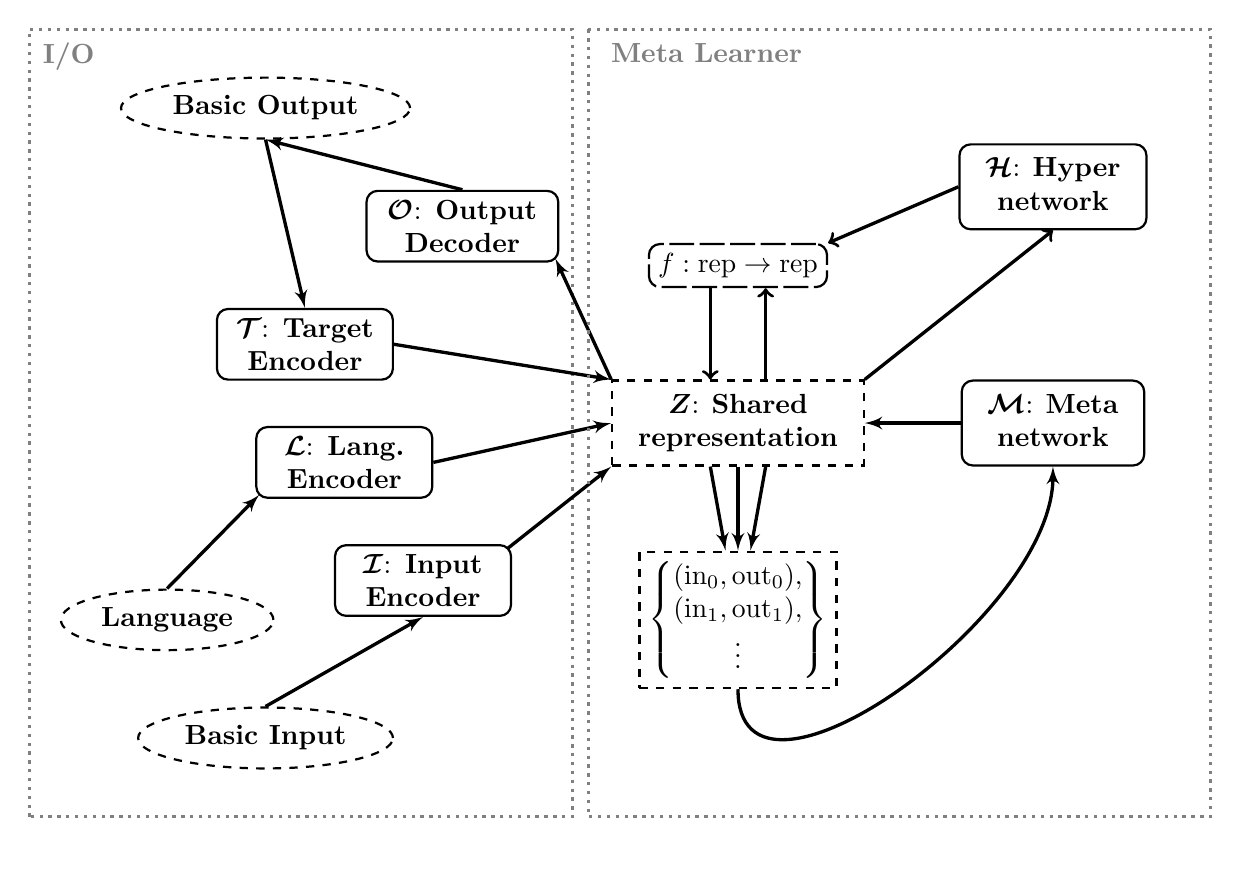
\begin{tikzpicture}[auto]

\node [dashblock] at (0, 0) (rep) {\begin{tabular}{c}$\bm{Z}$: \textbf{Shared} \\ \textbf{representation}\end{tabular}};

% inputs, outputs

\draw [boundingbox] (-9, -5) rectangle (-2.1, 5);
\node [text=gray] at (-8.5, 4.65) {\textbf{I/O}};

\node [conc] at (-6, -4) (perc) {\textbf{Basic Input}};
\node [conc] at (-7.25, -2.5) (lang) {\textbf{Language}};
\node [conc] at (-6, 4) (act) {\textbf{Basic Output}};
\node [block, text width=2cm] at (-4, -2) (IE) {$\bm{\mathcal{I}}$: \textbf{Input Encoder}};
\node [block, text width=2cm] at (-5, -0.5) (LE) {$\bm{\mathcal{L}}$: \textbf{Lang. Encoder}};
\node [block, text width=2.2cm] at (-3.5, 2.5) (OD) {$\bm{\mathcal{O}}$: \textbf{Output Decoder}};
\node [block, text width=2cm] at (-5.5, 1) (TE) {$\bm{\mathcal{T}}$: \textbf{Target Encoder}};
\path [line] (perc.north) to (IE.south);
\path [line] (lang.north) to ([xshift=0.05cm, yshift=0.05cm]LE.south west);
\path [line] ([xshift=-0.05cm, yshift=-0.05cm]IE.north east) to (rep.south west);
\path [line] (LE.east) to (rep.west);
\path [line] (rep.north west) to ([xshift=-0.05cm, yshift=0.05cm]OD.south east);
\path [line] (OD.north) to (act.south);
\path [line] (act.south) to (TE.north);
\path [line] (TE.east) to (rep.north west);

% meta
\draw [boundingbox] (-1.9, 5) rectangle (6, -5);
\node [text=gray] at (-0.4, 4.7) {\textbf{Meta Learner}};

\node [dashblock] at (0, -2.5) (collection) {
\(\left\{
\begin{matrix}
(\text{in}_0, \text{out}_0),\\
(\text{in}_1, \text{out}_1),\\
$\vdots$
\end{matrix}\right\}\)};
\path [line] (rep.south) to (collection);
\path [line] ([xshift=-1em]rep.south) to (collection);
\path [line] ([xshift=1em]rep.south) to (collection);

\node [block] at (4, 0) (meta) {\begin{tabular}{c}$\bm{\mathcal{M}}$: \textbf{Meta} \\ \textbf{network}\end{tabular}};
\path [line] (collection.south) to [out=-90, in=-90] (meta.south);
\path [line] (meta.west) to (rep.east);

% hyper

\node [block] at (4, 3) (hyper) {\begin{tabular}{c}$\bm{\mathcal{H}}$: \textbf{Hyper} \\ \textbf{network}\end{tabular}};
\node [block, dash pattern=on 9pt off 2pt] at (0, 2) (transform) {\(f: \text{rep} \rightarrow \text{rep}\)};

\path [draw, ->, very thick] (rep.north east) to (hyper.south);
\path [draw, ->, very thick] (hyper.west) to (transform.north east);
\path [draw, ->, very thick] ([xshift=-1em]transform.south) to ([xshift=-1em]rep.north);
\path [draw, ->, very thick] ([xshift=1em]rep.north) to ([xshift=1em]transform.south);

\end{tikzpicture}
\caption{Schematic of our general architecure. Blocks with solid edges denote deep networks with learnable parameters, dashed edges represent inputs, outputs, embeddings, etc., and $f$ is a deep network with parameters specified by $\mathcal{H}$.} \label{architecture_fig}
\end{figure}
More formally, we take a \textbf{functional} perspective on learning. A datum can be represented by a constant function which outputs it. (For example, each point in the latent space of an autoencoder can be thought of this way.) This allows us to interpret model inputs or outputs as functions. \par
We can then interpret most machine learning tasks as a mapping of functions to functions. These functions could represent data\footnote{Where ``data'' is a quite flexible term. The approach is relatively agnostic to whether the learning is supervised or reinforcement learning, whether inputs are images or natural language, etc.}, or they could be functions that operate on functions themselves. Under this perspective, learning tasks and learning to flexibly map between tasks, or learning to map from language to tasks, are all the same type of problem. \par
Specifically, we embed inputs, targets, and mappings into a shared representational space $Z$. Inputs are embedded by a deep network $\mathcal{I}: \text{input} \rightarrow Z$. Outputs are decoded from the representational space by a deep network $\mathcal{O}: Z \rightarrow \text{output}$. Targets are encoded by a deep network $\mathcal{T}: \text{targets} \rightarrow Z$. (Targets do not necessarily need to be output-like, e.g. in our RL tasks, we use (action, outcome) tuples as ``targets.'') \par
Given this, the task of mapping inputs to outputs can be framed as trying to find a transformation of the representational space that takes the (embedded) inputs from the training set to the (embedded) targets. These transformations are performed by a system with the following components:
\begin{itemize}
\item $\mathcal{M}: \{(Z, Z), ...\} \rightarrow Z $ -- the meta network, which takes a set of (input embedding, target embedding) pairs and produces a function embedding.
\item $\mathcal{H}: Z \rightarrow \text{parameters}$ -- the hyper network, which takes a function embedding and produces a set of parameters.
\item $f: Z \rightarrow Z$ -- the transformation, implemented by a deep network with parameters specified by $\mathcal{H}$.
\end{itemize}
See Fig. \ref{architecture_fig} for a schematic of the architecture. \par
\textbf{Operation:} A basic forward pass through the system might look as follows.
\begin{enumerate}
\item A training dataset of (input, target) pairs is embedded by $\mathcal{I}$ and $\mathcal{T}$ to produce a set of paired embeddings. Another set of (possibly unlabeled) inputs is provided and embedded.
\item The meta network $\mathcal{M}$ maps the set of embedded (input, target) pairs to a function embedding.
\item The hyper network $\mathcal{H}$ maps the function embedding to parameters for $f$, which is used to transform the second set of inputs to a set of output embeddings.
\item The output embeddings are decoded by $\mathcal{O}$ to produce a set of outputs.
\end{enumerate}
To write this explicitly, suppose we have some dataset of input, target pairs ($D_1 = \{(x_0, y_0), ...\}$), and some input $x$ for which we wish to generate a predicted output $\hat{y}$. This output would be generated as follows:
$$\hat{y} = \mathcal{O}\left(f_{D_1}\left(\mathcal{I} \left(x\right)\right) \right)$$
where $f_{D_1}$ is the transformation the meta-learner guesses for the training dataset $D_1$:
$$f_{D_1} \text{ is parameterized by } \mathcal{H}\left(\mathcal{M}\left( \left\{\left(\mathcal{I}\left(x_0\right), \mathcal{T}\left(y_0\right) \right), \left(\mathcal{I}\left(x_1\right), \mathcal{T}\left(y_1\right) \right), ... \right\}\right)\right)$$
This system can be trained end-to-end if labels are provided for a second set of inputs. In particular, suppose we have some loss function $\mathcal{L}(y, \hat{y})$ defined on a single target output $y$ and actual model output $\hat{y}$, for some input $x$. We define our total loss computed on some dataset $D_2$ as:
$$\mathbb{E}_{(x, y)\in {D}_2} \left[ \mathcal{L}\left(y, \mathcal{O}\left(f_{D_1}\left(\mathcal{I} \left(x\right)\right) \right)\right)\right]$$
More generally, suppose we have some input which is already embedded in the representation space $z_{in} \in Z$, and an embedded dataset $D_Z$ of (embedding, target embedding) pairs $\{(z_{in,0}, z_{out,0})\}$. Then we can generate an output $\hat{z}_{out} \in Z$ as:
$$\hat{z}_{out} = f_{D_Z}(z_{in}) \qquad \text{where } f_{D_Z} \text{ is parameterized by } \mathcal{H}\left(\mathcal{M}\left(D_Z\right)\right)$$
This output can then be appropriately dispatched depending on the task at hand. For example, if the $z_{in,i}$ are the system's embeddings for trying to win various games, and the $z_{out,i}$ are the corresponding embeddings for trying to lose those games, then $z_{out}$ could be interpreted as the system's guess at a losing strategy for the game embedded as $z_{in}$, and then could be used to play that game. We could then evaluate performance by how well the system actually performs at losing with the $z_{out}$ strategy. \par
Similarly, we could map from language to a task embedding, and then ask how well the system performs at the task specified by language. The key feature of our architecture -- the fact that tasks, data, and language are all embedded in a shared space -- allows substantial flexibility within a unified system.



\subsection{Results \& future directions}

\textbf{Results:} Briefly, the system is able to do meta-learning in a toy card-game domain I've constructed, that is, it's able to learn a held-out game from seeing a single batch of examples. It's also able to do mapping of tasks, such as trying to lose (based on task-mapping examples), even on held-out games. It can also achieve some success at these behaviors based on natural language input, although it generalizes less well from that than from examples. This is not too surprising, as the structure of a task is more directly captured by examples than by a symbolic encoding. \par 
\textbf{Future directions:}
There are a number of future directions I would like to explore:
\begin{itemize}
\item Can we find a task that demonstrates the ability of this architecture to perform comparably to humans, like OmniGlot \citep{Lake2015} but for more general flexibility?
\item Is there a way we can do unsupervised learning in the latent representation space that would approximate something like rerepresentation \citep{Karmiloff-Smith1986}? Could we do something to generate hypotheses or interesting experiments for active learning \citep{Markant2014a}? 
\item We've assumed knowledge of which experiences come from which tasks. However, this is an important learning problem in its own right, and it would be nice to try to solve it as well, perhaps with an approach similar to \citet{Achille2018}. 
\end{itemize}


\section{Towards a better understanding of human transfer and flexibility}
In this section I propose a set of behavioral experiments that will help us to probe the extent of human ability to transfer knowledge within an experimental session. This work builds off of work showing that humans can learn artificial grammars \citet{Cleeremans1991}, and can transfer this knowledge to isomorphic grammars with novel symbols \citep{Tunney2001}. It also builds off work on more complex graph-structure learning, starting with work by Anna Schapiro and colleagues \citep{Schapiro2013}, and continuing to more recent work showing that some graph structures are more learnable than others \citep{Kahn2018}. \par
The proposed experiment is as follows. We will have subjects perform two different tasks. The first will be analogous to the initial learning stage in \citet{Kahn2018}, and will consist of subjects trying to press key combinations in response to lit patterns of squares. Unbeknownst to them, these stimuli will come from a random walk on a structured graph. \citet{Kahn2018} showed that participants implicitly learned about the structure of this graph. After the first part of the experiment, participants will advance to a second part. This will be essentially analogous to the first, except that the cover task will be hitting single letters displayed on the screen, as in \citep{Cleeremans1991}. \par
We will experimentally manipulate the underlying graph structure which generates subjects stimuli in each stage of the experiment. In the first stage, subjects may either experience the modular structure of \citep{Schapiro2013} or a random graph which has the same number of nodes and edges (this will be randomly generated but fixed across subjects). See Fig. \ref{graph_struct_fig} for diagrams of the two structures. The structure in the second task will be crossed with this in a 2 x 2 design. We can thus examine whether there is a benefit to learning the second struture (i.e. more rapid learning and/or fewer mistakes) after an isomorphic graph as opposed to a non-isomorphic one.  \par
Finally, because I am interested in flexibility, we will also assess subjects' ability to explicitly reason about the structures they encountered. Specifically, we will reveal that the stimuli were generated from a structure, and give a subjects a two-alternative forced choice between the two structures, and ask them to pick which one they experienced in the second part of the experiment. We will also ask them to place the stimuli they encountered on this graph, and then evaluate how well they were able to explicitly reconstruct the true structure. \par

\subsection{Results and implications}
I believe this is an interesting study for a number of reasons. First, if we see transfer at the level of procedural performance, it will allow us to increase the upper bound on the complexity of structures which can be transferred over a short time scale. Prior work has shown that structures of this complexity can be learned, and that simpler structures can be transferred, but we are not aware of any work showing transfer effects with structures of this complexity. Second, the question of how we can reuse implicitly learned knowledge explicitly is underexplored. If subjects are not at chance on our explicit reasoning outcome measures, it will be interesting to investigate what predicts their performance on these questions. Both of these outcomes will help us to elucidate what sort of flexibility humans have when learning complex structures over short time scales. \par 
Furthermore, this work may have other implications for the literature. For example, \citet{Kahn2018} interpreted their results as showing that some structures are inherently more learnable than others. However, if we observe transfer benefits, an alternative interpretation would be that those results are due to the presence of structures more like this (hierarchical, clustery) in the world rather than any inherent learnability advantages. \par

\section{Conclusion}

In this paper, I have outlined a perspective on human flexibility and transfer. I have argued that flexibility and transfer arise from the interaction of complementary learning systems that learn across distinct timescales. These range from the slow accumulation of cultural knowledge, to our accumulation of statistical knowledge over our lifetimes, to our learning how to follow instructions. By leveraging our slowly-learned prior knowledge and our fast-learning systems, we are able to behave flexibly and learn rapidly in new situations. \par
I have related this cooperation between slow and fast learning systems to two different strategies for transfer in machine learning: multi-task learning and meta-learning. I have reviewed the literature on these topics, examined how it relates to human flexibility, and explored some human capabilities that are still missing. I have argued that combining different learning systems will be necessary to achieve more human-like flexibility. \par 
Building off this conceptual framework, I have outlined some of my prior work that explores the benefits of multi-task transfer in neural networks, and the benefits of multiple presentations in mathematical concept learning. I have also outlined a new study that will further explore the extent of human flexibility and transfer. Finally, I have proposed a new deep-learning architecture which combines fast and slow-learning systems to achieve more human-like flexibility. Taken together, I hope this research will shed more light on human learning and flexibility. \par 
\newpage
\bibliographystyle{apalike}
\bibliography{arrr}
\end{document}


\appendix

\chapter{Model details \& hyperparameters for all experiments} \label{appendix:model_hyperparameters}
\begin{figure}[h]
\begin{subfigure}{\textwidth}
\resizebox{\textwidth}{!}{%
\begin{tikzpicture}[auto]
%% from examples
\node[text width=0.5cm] at (-6.8, -0.5) (inputs0) {\includegraphics[width=0.5cm]{2-HoMM/figures/7_of_clubs.png}\\\includegraphics[width=0.5cm]{2-HoMM/figures/2_of_spades.png}};

\node[gray, text width=2cm, align=center] at (-5.6, 0.35) {Perception network};
\node[block] at (-5.6, -0.5) (perceptionnet0) {\(\mathcal{P}\)};
\path[arrow] (inputs0.east) -- ([xshift=-3]perceptionnet0.west);


\node[text width=0.5cm] at (-6.8, -2) (targets0) {\bf \color{red}\(-\)\$\$};

\node[gray, text width=2cm, align=center] at (-5.6, -2.85) {Target network};
\node[block] at (-5.6, -2) (targetnet0) {\(\mathcal{P}\)};
\path[arrow] ([xshift=3]targets0.east) -- ([xshift=-3]targetnet0.west);

\node[gray, text width=2.5cm, align=center] at (-3.25, 2.3) {Task examples (encoded)};
\node at (-3.25, 1.25) (examples) {
\(\left\{
\begin{matrix}
({\color{bgreen}z_{hand_{1}}}, {\color{bgreen}z_{bet_{1}}})\\
$\vdots$
\end{matrix}\right\}\)};

\path[arrow, out=0, in=-90] (perceptionnet0.east) to ([xshift=-11, yshift=20]examples.south);
\path[arrow, out=0, in=-90] (targetnet0.east) to ([xshift=15, yshift=20]examples.south);

\node[gray, text width=2cm, align=center] at (-0.5, 2.1) {Example network};
\node[block] at (-0.5, 1.25) (examplenet) {\(\mathcal{E}\)};
\path[arrow] (examples.east) -- ([xshift=-3]examplenet.west);

%% performing 
\node[bpurp] at (1.25, 1.25) (taskrep) {\(z_{task}\)};
\path[arrow] ([xshift=3]examplenet.east) -- (taskrep.west);

\node[gray, text width=2cm, align=center] at (3, 2.1) {Hyper network};
\node[block] at (3, 1.25) (hypernet) {\(\mathcal{H}\)};
\path[arrow] (taskrep.east) -- ([xshift=-3]hypernet.west);

\node[text width=0.5cm] at (0.7, -1.25) (inputs) {\includegraphics[width=0.5cm]{2-HoMM/figures/2_of_spades.png}\\\includegraphics[width=0.5cm]{2-HoMM/figures/4_of_hearts.png}};

\node[gray, text width=2cm, align=center] at (1.9, -0.4) {Perception network};
\node[block] at (1.9, -1.25) (perceptionnet) {\(\mathcal{P}\)};
\path[arrow] (inputs.east) -- ([xshift=-3]perceptionnet.west);

\node[bgreen] at (3.2, -1.25) (handrep) {\(z_{hand}\)};
\path[arrow] ([xshift=3]perceptionnet.east) -- (handrep.west);

\node[bblue, block, dashed] at (4.5, -1.25) (tasknet) {\(\mathcal{T}\)};
\node[bblue, text width=2cm, align=center] at (4.5, -2) {Task network};
\path[arrow] (handrep.east) -- ([xshift=-3]tasknet.west);
\path[arrow, out=0, in=90] ([xshift=3]hypernet.east) to ([yshift=3]tasknet.north);


\node[bgreen] at (5.65, -1.25) (betrep) {\(z_{bet}\)};
\path[arrow] ([xshift=3]tasknet.east) -- (betrep.west);

\node[gray, text width=2cm, align=center] at (6.8, -0.4) {Action network};
\node[block] at (6.8, -1.25) (actionnet) {\(\mathcal{A}\)};
\path[arrow] (betrep.east) -- ([xshift=-3]actionnet.west);

\node at (7.7, -1.25) (output) {\bf \$};
\path[arrow] ([xshift=3]actionnet.east) -- (output.west);

\node at (8.7, -1.25) (loss) {Loss};
\path[arrow] (output.east) -- (loss.west);

% gradients

\path[arrow, bred, ultra thick] ([yshift=-12, xshift=20]loss.west) to ([yshift=-12, xshift=3]inputs.east);

\path[draw, bred, ultra thick, out=90, in=0] ([yshift=-12, xshift=-10]tasknet.west) to ([yshift=-12, xshift=-10]hypernet.east);

\path[draw, bred, ultra thick] ([yshift=-12, xshift=-10]hypernet.east) to ([yshift=-12, xshift=-40]examples.east);

\path[draw, bred, ultra thick, out=-90, in=0] ([yshift=-12, xshift=-40]examples.east) to ([yshift=-12, xshift=-10]perceptionnet0.east);
\path[arrow, bred, ultra thick] ([yshift=-12, xshift=-10]perceptionnet0.east) to ([yshift=-12]inputs0.east);

\path[draw, bred, ultra thick, out=-90, in=0] ([yshift=-12, xshift=-12]examples.east) to ([yshift=-12, xshift=-10]targetnet0.east);
\path[arrow, bred, ultra thick] ([yshift=-12, xshift=-10]targetnet0.east) to ([yshift=-12]targets0.east);

\end{tikzpicture}
}
\caption{Basic task inference/training (from examples).} \label{supp_fig:HoMM:gradient_flow:basic_tasks}
\end{subfigure}
\begin{subfigure}{\textwidth}
\resizebox{\textwidth}{!}{%
\begin{tikzpicture}[auto]
%% from examples
\node at (-6.9, 0) {};

\node[gray, text width=3.5cm, align=center] at (-3.25, 2.3) {Mapping examples (input/output tasks)};
\node at (-3.25, 1.25) (examples){
\(\left\{
\begin{matrix}
({\color{bpurp}z_{chess}}, {\color{bpurp}z_{lose chess}})\\
$\vdots$
\end{matrix}\right\}\)};

\node[gray, text width=2cm, align=center] at (-0.5, 2.1) {Example network};
\node[block] at (-0.5, 1.25) (examplenet) {\(\mathcal{E}\)};
\path[arrow] (examples.east) -- ([xshift=-3]examplenet.west);

%% performing 
\node[borange] at (1.25, 1.25) (taskrep) {\(z_{meta}\)};
\path[arrow] ([xshift=3]examplenet.east) -- (taskrep.west);

\node[gray, text width=2cm, align=center] at (3, 2.1) {Hyper network};
\node[block] at (3, 1.25) (hypernet) {\(\mathcal{H}\)};
\path[arrow] (taskrep.east) -- ([xshift=-3]hypernet.west);

\node[bpurp] at (2.66, -1.25) (handrep) {\(z_{poker}\)};

\node[bblue, block, dashed] at (4.5, -1.25) (tasknet) {\(\mathcal{T}\)};
\node[bblue, text width=2cm, align=center] at (4.5, -2) {Task network};
\path[arrow] (handrep.east) -- ([xshift=-3]tasknet.west);
\path[arrow, out=0, in=90] ([xshift=3]hypernet.east) to ([yshift=3]tasknet.north);

\node[bpurp] at (6.5, -1.25) (output) {\(\hat{z}_{lose poker}\)};
\path[arrow] ([xshift=3]tasknet.east) -- (output.west);

\node at (8.7, -1.25) (loss) {Loss};
\path[arrow] (output.east) -- (loss.west);

% gradients

\path[arrow, bred, ultra thick] ([yshift=-12, xshift=20]loss.west) to ([yshift=-12, xshift=5]handrep.east);

\path[draw, bred, ultra thick, out=90, in=0] ([yshift=-12, xshift=-10]tasknet.west) to ([yshift=-12, xshift=-10]hypernet.east);

\path[arrow, bred, ultra thick] ([yshift=-12, xshift=-10]hypernet.east) to ([yshift=-12, xshift=10]examples.east);
\end{tikzpicture}
}
\caption{Meta-mapping inference/training (from examples).}\label{supp_fig:HoMM:gradient_flow:meta_mappings}
\end{subfigure}
\caption[Schematic of architecture, showing inference and gradient flow through the model on a training step.]{Schematic of architecture, showing inference and gradient flow through the model on a training step. Thin lines moving rightward represent inference, thick red lines moving leftward represent gradients. (\subref{supp_fig:HoMM:gradient_flow:basic_tasks}) Inference and gradients for the basic tasks. (\subref{supp_fig:HoMM:gradient_flow:basic_tasks}) Inference and gradients for meta-mappings. The gradients end at the examples of the meta-mapping, rather than propagating through to alter how those representations are constructed, due to GPU memory constraints. In the future, it might be useful to explore whether allowing further propagation would improve results for both basic tasks and meta-mappings. (These figures depict the inference/gradient flow when performing tasks and meta-mappings from examples, performing from language is similar, except that the example inputs and example network are replaced with language inputs and the language processing network.)} \label{supp_fig:HoMM:gradient_flow}
\end{figure}

In Fig. \ref{supp_fig:HoMM:gradient_flow}, we show the flow of inference (forward) and gradients (backward) through the HoMM architecture on basic task and meta-mapping training steps.

\begin{table}
\scriptsize
\centering
\begin{tabular}{|p{3cm}||c|c|c|c|}
\hline
& Polynomials & Cards & Visual & RL \\\hline
\hline
$Z$-dimension & 512 & 512 & 512 & 512 \\\hline
$\mathcal{I}$ num. layers & \multicolumn{4}{c|}{2} \\\hline
$\mathcal{I}$ num. hidden units & \multicolumn{4}{c|}{128} \\\hline
$\mathcal{I}$ conv. layers. (num filters, size, all strides are 2) & \multicolumn{2}{c|}{-} & \multicolumn{1}{p{2.3cm}|}{(64, 5), (128, 4), (256, 4), (512, 2), max pool} & \multicolumn{1}{p{2.3cm}|}{(64, 7), (64, 4), (64, 3)}\\\hline
$\mathcal{L}$ architecture & -  & \multicolumn{3}{c|}{2-layer LSTM + 2 fully-connected} \\\hline
$\mathcal{L}$ num. hidden units & -  & \multicolumn{3}{c|}{512} \\\hline
$\mathcal{T}$ num. layers & 1 & 3 & 1 & 3 \\\hline
$\mathcal{T}$ num. hidden units & - & 128 & - & 128 \\\hline
$\mathcal{M}$ architecture & \multicolumn{4}{c|}{2 layers per-datum, max pool across, 2 layers} \\\hline
$\mathcal{H}$ architecture & \multicolumn{4}{c|}{4 layers} \\\hline
$\mathcal{M}$ num. hidden units & \multicolumn{3}{c|}{512} & 1024 \\\hline
$\mathcal{H}$ num. hidden units & \multicolumn{4}{c|}{512} \\\hline
Task, MM representations from & \multicolumn{2}{c|}{Examples} & Language & Examples \\\hline
$\mathcal{F}$ num. layers & 3 & 1 & HoMM: 1, Lang: 3 & 3 \\\hline
$\mathcal{F}$ num. hidden units & \multicolumn{3}{c|}{64} & 128 \\\hline
$\mathcal{F}$ init scale & 1 & 1 & 30 & 10 \\\hline
$\mathcal{F}$ weight norm. \citep{Salimans2016} & \multicolumn{3}{c|}{No} & Yes \\\hline
$\mathcal{A}$ num. layers & \multicolumn{2}{c|}{1} & 2 & 1 \\\hline
$\mathcal{A}$ num. hidden units & \multicolumn{2}{c|}{-} & 128 & -  \\\hline
Nonlinearities & \multicolumn{4}{p{11cm}|}{Leaky ReLU most places, except no non-linearity at final layer of networks outputting to $Z$, sigmoid for classification outputs, and softmax over actions.} \\\hline
Base task loss & $\ell_2$ & $\ell_2$ (masked) & Cross-entropy & $\ell_2$ (masked)\\\hline
Meta-mapping loss & \multicolumn{4}{c|}{$\ell_2$}\\\hline
Partially-persistent task embeddings & \multicolumn{3}{c|}{No} & Yes \\\hline
Persistent embedding match loss weight & \multicolumn{3}{c|}{-} & 0.2 \\\hline
\hline
Optimizer & Adam & \multicolumn{3}{c|}{RMSProp} \\\hline
Learning rate (base) & $3\cdot 10^{-5}$ & $1\cdot 10^{-5}$ & $3\cdot 10^{-5}$ & $1\cdot 10^{-4}$\\\hline
Learning rate (meta) & $1\cdot 10^{-5}$ & $1\cdot 10^{-5}$ & $1\cdot 10^{-5}$ & $1\cdot 10^{-4}$\\\hline
L.R. decay rate (base) & $\times0.85$ & $\times0.85$ & $\times0.8$ & $\times0.8$\\\hline
L.R. decay rate (meta) & $\times0.85$ & $\times0.9$ & $\times0.85$ & $\times0.95$ \\\hline
L.R. min (base) & \multicolumn{2}{c|}{$3 \cdot 10^{-8}$}  & $1 \cdot 10^{-8}$ & $3 \cdot 10^{-8}$\\\hline
L.R. min (meta) & $1 \cdot 10^{-7}$& $3 \cdot 10^{-8}$ &  $1 \cdot 10^{-8}$ & $3 \cdot 10^{-7}$\\\hline
L.R. decays every & 100 epochs & 200 epochs & 400 epochs & 10000 \\\hline
Num. training epochs & 5000 & \multicolumn{1}{p{2.3cm}|}{100000 (optimally stopped)} & \multicolumn{1}{p{2.3cm}|}{10000 for 4 train mappings, 7500 for 8, 5000 for others} & \multicolumn{1}{p{2.3cm}|}{300000 (optimally stopped)} \\\hline
Num. runs & 5 & 5 & 10 & 5 \\ \hline
\hline
Num. base tasks (training) & \multicolumn{1}{p{2.3cm}|}{1300 ( $= 60 + 60 \times  20 + 40$)} & 36 & Varies & 18 \\\hline
Num. base tasks (held out for MM eval) & 800 ($= 40 \times 20$)  & 4 & Varies & 2 \\\hline
Num. meta classifications & 6 & 8 & 8 & - \\\hline
Num. train MMs & 20 & 3 & Varies & 1 \\\hline
Num. held-out MMs & 16 & 0 & 2 & 0  \\\hline
Base dataset size & 1024 & 1024 & 336 & 64 \\\hline
Base examples size & 50 & 768 & - & 32 \\\hline
Meta dataset size (train) & 60 & 36 & Varies & 18 \\\hline
Meta examples (train) & \multicolumn{2}{c|}{Half of train dataset} & - & Half of train dataset \\\hline
Meta examples (eval) & \multicolumn{2}{c|}{All of train dataset} & - & All of train dataset \\\hline
Base datasets refreshed & \multicolumn{2}{c|}{Every 50 epochs} & Every 20 & Every 1500  \\\hline
Target network updated & \multicolumn{3}{c|}{-} & Every 10000 epochs  \\\hline
RL discount & \multicolumn{3}{c|}{-} & 0.85 \\\hline
RL explore prob. (\(\epsilon\)) & \multicolumn{3}{c|}{-} & \multicolumn{1}{p{2.5cm}|}{Init: 1, decay: -0.03}\\\hline
Action softmax \(\beta\) & - & 8 & - & 8\\\hline
\end{tabular}
\caption[Detailed hyperparameter specification.]{Detailed hyperparameter specification for different experiments. A ``-'' indicates a parameter that does not apply to that experiment. As a reminder: the shared representational space is denoted by $Z$. Input encoder: $\mathcal{I}: \text{input} \rightarrow Z$. Action decoder $\mathcal{A}: Z \rightarrow \text{output}$. Target encoder $\mathcal{T}: \text{targets} \rightarrow Z$. Meta-network $\mathcal{M}: \{(Z, Z), ...\} \rightarrow Z $ maps examples to a task representation. Hyper-network $\mathcal{H}: Z \rightarrow \text{parameters}$. Task network $F: Z \rightarrow Z$ is parameterized by $\mathcal{H}$. Language encoder: $\mathcal{L}: \text{language} \rightarrow Z$. } \label{supp_hyperparameter_table}
\end{table}
See table \ref{supp_hyperparameter_table} for detailed architectural description and hyperparameters for each experiment. Hyperparameters were generally found by a heuristic search, where mostly only the optimizer, learning rate annealing schedule, and number of training epochs were varied. Some of the parameters take the values they do for fairly arbitrary reasons, e.g. the polynomial experiments were run earlier, before 1-layer task networks were found to be useful in some settings. While it would be ideal to fully search the space of parameters for all models, unfortunately our computational resource limitations prohibited it. Thus the results in the paper should be interpreted as a lower bound on what would be possible. \par
Each epoch consisted of a separate learning step on each task (both base and meta), in a random order. In each task, the meta-learner would receive only a subset (the ``batch size`` above) of the examples to generate a function embedding, and would have to generalize to the remainder of the examples in the dataset. The embeddings of the basic tasks used for meta-mappings were computed and cached once per epoch, so as the network learned over the course of the epoch, these task-embeddings would get ``stale,'' but this did not seem to be too detrimental. In the case of the RL tasks, where there were persistent task embeddings, they were used insteadd.\par
The results reported in the figures in this paper are averages across multiple runs, with different trained and held-out tasks (in the polynomial and visual concepts cases) and different network initializations and training orders each epoch (in all cases), to ensure the robustness of the findings. \par

\subsubsection{Source repositories}
%The full code for all experiments and analyses will be made available via github in the de-anonymized verison.
The full code for the experiments and analyses can be found on github:
\begin{itemize}
\item HoMM library: \url{https://github.com/lampinen/HoMM}
%\item This paper's source: \url{https://github.com/lampinen/metamapping_paper}
\item Polynomials: \url{https://github.com/lampinen/HoMM_polynomial_analysis}
\item Cards (models): \url{https://github.com/lampinen/HoMM_cards}
\item Cards (human experiment): \url{https://github.com/lampinen/cards_for_humans}
\item Concepts: \url{https://github.com/lampinen/categorization_HoMM}
\item RL: \url{https://github.com/lampinen/HoMM_grids}
\item Stroop results (below): \url{https://github.com/lampinen/stroop}
\end{itemize}



\section{Clarifying meta-mapping} \label{app_clarifying_meta_mapping}
\subsection{A definitional note}
When we discussed meta-mappings in the main text, we equivocated between tasks and behaviors for the sake of brevity. For a perfect model, this is somewhat justifiable, because each task will have a corresponding optimal behavior, and the sytem's embedding of the task will be precisely the embedding which produces this optimal behavior. However, behavior-irrelevant details of the task, like the color of the board, may not be embedded, so this should not really be thought of as a task-to-task mapping. This problem is exacerbated when the system is imperfect, e.g. during learning. It is thus more precise to distinguish between a ground-truth meta-mapping, which maps tasks to tasks, and the computational approach to achieving that meta-mapping, which really maps between representations which combine both task and behavior. \par



\chapter{Supplemental material for Chapter \getrefnumber{chapter:zero_shot_via_homm}} \label{appendix:zero_shot_via_homm}

\section{Details of polynomial task domain} \label{app:HoMM:polynomials_methods}
We randomly sampled the train and test polynomials as follows:
\begin{enumerate}
\item Sample the number of relevant variables ($k$) uniformly at random from 0 (i.e. a constant) to the total number of variables.
\item Sample the subset of $k$ variables that are relevant from all the variables.
\item For each term combining the relevant variables (including the intercept), include the term with probability 0.5. If so give it a random coefficient drawn from $\mathcal{N}(0, 2.5)$.
\end{enumerate}
The data points on which these polynomials were evaluated were sampled uniformly from $[-1, 1]$ independently for each variable, and for each polynomial. The datasets were resampled every 50 epochs of training. \par
\textbf{Meta-tasks:} For meta-tasks, we trained the network on 6 task-embedding classification tasks:
\begin{itemize}
\item Classifying polynomials as constant/non-constant.
\item Classifying polynomials as zero/non-zero intercept.
\item For each variable, identifying whether that variable was relevant to the polynomial.
\end{itemize}
We trained on 20 meta-mapping tasks, and held out 16 related meta-mappings.
\begin{itemize}
\item Squaring polynomials (where applicable).
\item Adding a constant (trained: -3, -1, 1, 3, held-out: 2, -2).
\item Multiplying by a constant (trained: -3, -1, 3, held-out: 2, -2).
\item Permuting inputs (trained: 1320, 1302, 3201, 2103, 3102, 0132, 2031, 3210, 2301, 1203, 1023, 2310, held-out: 0312, 0213, 0321, 3012, 1230, 1032, 3021, 0231, 0123, 3120, 2130, 2013).
\end{itemize}


%\section{Card game $t$-SNE} \label{app_cards_tsne}
%We performed $t$-SNE \citep{LaurensvanderMaaten2008} on the task embeddings of the system at the end of learning the card game tasks, to evaluate the organization of knowledge in the network. In fig. \ref{fig_cards_tsne_basic} we show these embeddings for just the basic tasks. The embeddings show systematic grouping by game attributes. In fig. \ref{fig_cards_tsne_full} we show the embeddings of the meta and basic tasks, showing the organization of the meta-tasks by type. (Note: this analysis was performed in an older version of the model than the main results.)\par 
%\begin{figure}[H]
%\centering
%\includegraphics[width=0.8\textwidth]{2-HoMM/figures/basic_tsne_basic_final.png}
%\caption{$t$-SNE embedding of the function embeddings the system learned for the basic card game tasks. (Note that the pairs of nearby embeddings differ in the ``suits rule`` attribute, discussed in appendix \ref{meth_data_cards}.)} 
%\label{fig_cards_tsne_basic}
%\end{figure}%
%\begin{figure}[H]
%\centering
%\includegraphics[width=0.9\textwidth]{2-HoMM/figures/basic_tsne_full_final.png}
%\caption{$t$-SNE embedding of the function embeddings the system learned for the meta tasks (basic tasks are included in the background).} 
%\label{fig_cards_tsne_full}
%\end{figure}

\section{Architecture \& training experiments} \label{app_lesion_results}
In this section we consider a few variations of the architecture and training, to justify the choices made in the paper. \par

\subsection{Shared $Z$ vs. separate task-embedding and data-embedding space} \label{app_lesion_results_shared_z}
Instead of having a shared $Z$ where data and tasks are embedded, why not have a separate embedding space for data, tasks, and so on? There are a few conceptual reason why we chose to have a shared $Z$, including its greater parameter efficiency, the fact that humans seem to represent our conscious knowledge of different kinds in a shared space \citep[][]{Baars2005}, and the fact that this representation could allow for zero-shot adaptation to new computational pathways through the latent space, analogously to the zero-shot language translation results reported by Johnson and colleagues \citep{Johnson2016a}. In this section, we further show that training with a separate task encoding space worsens performance, see fig. \ref{supp_lesion_shared_z_fig}. This seems to primarily be due to the fact that learning in the shared $Z$ accelerates and de-noises the learning process, see fig. \ref{supp_lesion_shared_z_learn_fig}. (It's therefore worth noting that running this model for longer could result in convergence to the same asymptotic generalization performance.) Note: this analysis was performed in an older implementation of the model. \par
\begin{figure}[H]
\centering
\includegraphics[width=\textwidth]{2-HoMM/figures/poly/meta_results_unshared_vs_shared.png}
\caption[Having a separate embedding space for tasks results in worse performance on meta-mappings.]{Having a separate embedding space for tasks results in worse performance on meta-mappings. (Results are from only 1 run.)}
\label{supp_lesion_shared_z_fig}
\end{figure}

\begin{figure}[H]
\centering
\includegraphics[width=\textwidth]{2-HoMM/figures/poly/meta_learning_curves_with_separate.png}
\caption[Having a separate embedding space for tasks results in noisier, slower learning of meta-mappings.]{Having a separate embedding space for tasks results in noisier, slower learning of meta-mappings. (Results are from only 1 run.)}
\label{supp_lesion_shared_z_learn_fig}
\end{figure}

\subsection{Hyper network vs. conditioned task network} \label{app_lesion_results_hyper}
Instead of having the task network $F$ parameterized by the hyper network $\mathcal{H}$, we could simply have a task network with learned weights which takes a task embedding as another input. In Fig. \ref{supp_fig:HoMM_arch_cond_vs_hyper}, we show that this architecture fails to learn the meta-mapping tasks, although it can successfully perform the basic tasks. We suggest that this is because it is harder for this architecture to prevent interference between the comparatively larger number of basic tasks and the smaller number of meta-tasks. While it might be possible to succeed with this architecture, it was more difficult in the hyper-parameter space we searched. See also Fig. \ref{supp_fig:human:lang_tcnh}, where we show that both architectures perform similarly for language generalization. \par 

\begin{figure}[H]
\centering
\includegraphics[width=0.5\textwidth]{2-HoMM/figures/conditioned_vs_hyper_polynomials.png}
\caption[The HyperNetwork-based architecture we propose outperforms a simpler architecture.]{The HyperNetwork-based architecture we propose in the main text performs better and more consistently on meta-mappings than a simpler architecture that simply concatenates a task representation to the input before passing it through a fixed MLP. Results are in the polynomial domain, c.f. Fig. \ref{fig:HoMM_polynomials:results}. Note that the task-concatenated architecture performs just as well at the trained basic tasks (not shown), it is adapting via meta-mappings that proves challenging for it. See Supp. Fig. \ref{supp_fig:extending:RL:arch_cond_vs_hyper} for a more dramatic comparison in the RL domain. }\label{supp_fig:HoMM_arch_cond_vs_hyper}
\end{figure}

\subsection{Meta-classification lesion} \label{app:homm:metaclass_lesion}

In Fig. \ref{supp_fig:HoMM:metaclass_lesion}, we show that meta-classification training is not beneficial in the polynomials domain. Specifically, on trained meta-mappings the HoMM model is achieving a normalized performance of 88.99\% (bootstrap 95\%-CI [88.20, 89.98]), while without meta-classification it is achieving a normalized performance of 89.7\% (bootstrap 95\%-CI [88.87, 90.61]). On new meta-mappings the HoMM model is achieving a normalized performance of 85.54\% (bootstrap 95\%-CI [85.14, 85.94]), while without meta-classification it is achieving a normalized performance of 86.29\% (bootstrap 95\%-CI [85.54, 86.79]). While these differences are significant (paired \(t\)-tests, respectively \(t(4) = 6.95, p = 0.002\) and \(t(4) = 3.06, p = 0.038\)), the effect is small. See also Fig. \ref{supp_fig:human:homm_metaclass_lesion} for marginal evidence that meta-classification may be helpful in the cards domain, where there are fewer training tasks. 

\begin{figure}[H]
\centering
\includegraphics[width=0.5\textwidth]{2-HoMM/figures/metaclass_lesion_polynomials.png}
\caption[In the polynomials domain, the HoMM model performs slightly better without meta-classification training.]{In the polynomials domain, the HoMM model performs slightly better without meta-classification training. This effect appears for both trained and held-out meta-mappings. However, the effect is small.}\label{supp_fig:HoMM:metaclass_lesion}
\end{figure}


\chapter{Supplemental material for chapter \getrefnumber{chapter:human}} \label{appendix:human}

\section{Details of human experiment}
The experiment was implemented online, and run on Amazon Mechanical Turk. The code was based on the jsPsych library \citep{DeLeeuw2015}. The full code for the experiment and analysis can be found at \url{https://github.com/lampinen/cards_for_humans}. In this section we provide some details in a more easily readable format.

\subsection{Detailed experiment outline}

\subsubsection{Introduction \& rules}
\begin{itemize}
\item Page 1:
    \begin{itemize}
    \item Hi, welcome to our HIT. We are researchers from the Stanford Department of Psychology, conducting an experiment on game playing.
    \item The first part of this experiment should take 5-10 minutes. The base pay is \$1, and if you pass the end of the first phase, there will be a second phase that will take about 10 minutes. You will be paid a bonus of \$1.50 for making it to this second phase, there will be an extra bonus based on performance in the second phase.
    \item If you do not wish to participate, you may return the HIT at any time, but you will not be compensated unless you complete it.
    \end{itemize}
\item  Page 2:
    \begin{itemize}
    \item If you make it to the second phase of the experiment, you'll be playing a simple card game. In this first phase of the experiment, you'll learn the rules.
    \item We'll test your understanding of the rules at the end of the first phase, and if you pass you'll make it to the second phase, where you'll earn a \$1 bonus + an extra performance bonus.
    \item Make sure you follow all instructions very carefully, in order to make it to the second phase of the experiment and earn the maximum bonus pay.
    \end{itemize}
\item  Page 3:
    \begin{itemize}
    \item In the card game, you will receive a hand of two cards, each of which has a number (1-4) and a color (red or black). There are several decks in play, so there are multiple copies of each card, and two or more can appear in the same round.
    \end{itemize}
\item  Page 4:
    \begin{itemize}
    \item You will be playing against an opponent, trying to win money. You'll get to make a bet of 0, 5, or 10 cents.
    \item If your hand beats your opponent's hand, you will win the amount you bet. If your opponent wins, you'll lose the amount you bet. If you bet nothing, you won't win or lose anything. Also, if you tie, you won't win or lose either.
    \item In the second phase, we'll pay you a bonus equal to your net earnings (or 0 if your earnings are negative), on top of the \$1 bonus for making it to the second phase."
    \end{itemize}
\item  Page 5:
    \begin{itemize}
    \item In the card game, \textbf{the best types of hands are two adjacent numbers of the same color}, for example black 2 and black 3.
    \item \textbf{The next best hands are those with two adjacent numbers of different color,} for example black 3 and red 4.
    \item \textbf{The worst types of hands are those with matching numbers or non-adjacent numbers}, like 4, 4 or 1, 3.
    \item \textbf{Hands of better types always beat worse hands.}
    \end{itemize}
\item  Page 6:
    \begin{itemize}
    \item \textbf{If two hands are of the same type, the one with the highest card wins.} If the highest cards of the two hands tie, the tie is broken by the lower cards.
    \item \textbf{If both cards are tied, black cards beat red cards,} highest first, lowest if the high cards are the same color. If the hands are perfectly tied, you don't win or lose money.
    \end{itemize}
\end{itemize}

\subsubsection{Game understanding check}
\begin{itemize}
\item Instructions:
    \begin{itemize}
    \item We'll now test your understanding by giving you a few example pairs of hands. Just click on the hand from each pair that would win. \textbf{\color{red} If you make more than one mistake in this section, the experiment will end. Make sure you fully understand the instructions before proceeding, otherwise you may not make it to the second phase!}
    \item If you need to, you can go back to the earlier instructions to refresh your memory before proceeding.
    \item Click next to start the test.
    \end{itemize}
\item Trials (see fig. \ref{fig:appdx_human_comparison_trial}, hand position was randomized):
    \begin{itemize}
        \item black 3 and red 2 vs. red 4 and 1. Explanation: "Adjacent cards beat non-adjacent." 
        \item red 1 and 2 vs. red 4 and black 3. Explanation: "Same-suit adjacent beats different suit." 
        \item black 3 and red 3 vs. red 4 and 1. Explanation: "Highest card breaks ties." 
        \item black 4 and 3 vs. red 4 and 3. Explanation: "Black cards beat red cards if the numbers are tied." 
    \end{itemize}
\item Evaluation: If the participants got 3 out of 4 trials correct, they passed. 
    \begin{itemize}
        \item \textbf{Passed:} Congratulations, you passed the test, and will get to proceed to phase 2! You have earned a \$1.50 bonus, and will be awarded a performance bonus based on your bets in the next phase. Press any key to continue.
        \item \textbf{Failed:} Sorry, you made more than one mistake, and did not pass the test. The experiment will now end. Press any key to continue.
    \end{itemize}
\end{itemize}

\begin{figure}
\centering
\includegraphics[width=0.75\textwidth]{3-human-adaptation/figures/comparison_correct.png}
\caption{An example hand-comparison trial from the understanding check.} \label{fig:appdx_human_comparison_trial}
\end{figure}

\subsubsection{Block 1: with feedback}
\begin{itemize}
\item Instructions:
    \begin{itemize}
    \item Now you get to play a few hands. After you bet, we'll show you your opponent's hand and how much you won (or lost), and at the end of these hands we'll tell you your total earnings. Press any key to continue.
    \end{itemize}

\item Trials:
    \begin{itemize}
    \item 32 trials of playing the game and seeing the result of each hand, with the participants hand distributed evenly across 16 bins of hand win probability. Opponents hands were randomly sampled. 
    \end{itemize}
\item Block end:
    \begin{itemize}
    \item Participants were shown their block earnings, as well as their total earnings so far.
    \end{itemize}
\end{itemize}

\subsubsection{Block 2: without feedback}
\begin{itemize}
\item Instructions:
    \begin{itemize}
    \item To test how well you understand the game, we'll now give you a series of hands where you won't see your results after you bet. You will just see your earnings at the end of the set of hands. Press any key to continue.
    \end{itemize}
\item Trials:
    \begin{itemize}
    \item 24 trials of playing the game with the result grayed out, with the participants hand distributed evenly across 8 bins of hand win probability. Opponents hands were not sampled, participants were paid their expected earnings for each hand, with the final block total rounded to the closest 10 cents. 
    \end{itemize}
\item Block end:
    \begin{itemize}
    \item Participants were shown their block earnings, as well as their total earnings so far.
    \end{itemize}
\end{itemize}

\subsubsection{Block 3: losing variation, no feedback}
\begin{itemize}
\item Instructions:
    \begin{itemize}
    \item \textbf{\color{red} Now, we want you to try to lose the game! For the remainder of the experiment, if you bet and lose, you'll gain the amount you bet, and if you bet and win, you'll lose the amount you bet.}
    \item As before, you won't win or lose anything if you tie your opponent, or if you don't bet.
    \item Press any key to continue.
    \end{itemize}
\item Attention check:
    \begin{itemize}
    \item To make sure you understand, please answer this question. From now on, I will earn money if I:
    \item ``Bet and my hand wins.'', ``Bet and my hand loses.'' 
    \end{itemize}
\item Instructions 2:
    \begin{itemize}
    \item Great, now you get to play a few hands! As before, you won't see your results after you bet. You will just see your earnings at the end of the set of hands. Press any key to continue.
    \end{itemize}
\item Trials:
    \begin{itemize}
    \item 24 trials of playing the game with the result grayed out, with the participants hand distributed evenly across 8 bins of hand win probability. Opponents hands were not sampled, participants were paid their expected earnings for each hand, with the final block total rounded to the closest 10 cents. 
    \end{itemize}
\item Block end:
    \begin{itemize}
    \item Participants were shown their block earnings, as well as their total earnings so far.
    \end{itemize}
\end{itemize}

\subsubsection{Debrief}
We asked participants about their age, education, gender, and race/ethnicity. However, we did not analyze these data.


\section{Results of the human experiment}
\subsection{Suboptimality}\label{appendix:human:suboptimality}
As \citet{Jarvstad2013} note, how ``optimal'' human performance seems to be depends on how you measure performance. In particular, performance seems better when measured in terms of expected earnings than when measured in terms of how accurately participants decided whether or not to bet (fig. \ref{fig:appx_human_calibration}). This is because the participants were more accurate on trials with higher (absolute) expected value, and less accurate on trials where they had less to gain or lose. We chose the more optimistic performance measure as the basis for our comparison to the HoMM model.
\begin{figure}[H]
\centering
\begin{subfigure}[t]{0.5\textwidth}
\includegraphics[width=\textwidth]{3-human-adaptation/figures/human_adaptation_supp_earnings.png}
\caption{Performance measured in terms of earnings.}
\end{subfigure}%
\begin{subfigure}[t]{0.5\textwidth}
\includegraphics[width=\textwidth]{3-human-adaptation/figures/human_adaptation_supp_accuracy.png}
\caption{Performance measured in terms of accuracy, i.e. the percent of hands where an optimal decision was made}
\end{subfigure}%
\caption{How close human perforance seems to optimal depends on your metric.} \label{fig:appx_human_calibration}
\end{figure}


\section{Details of model tasks \& training}\label{app:human:model_details}
\subsection{Tasks}

Our card games were played with two suits, and 4 values per suit. In our setup, each hand in a game has a win probability (proportional to how it ranks against all other possible hands). The agent is dealt a hand, and then has to choose to bet 0, 1, or 2 (the three actions it has available). We considered a variety of games which depend on different features of the hand:
\begin{itemize}
\item \textbf{Straight flush:} Most valuable is adjacent numbers in same suit, i.e. 4 and 3 in most valuable suit (royal flush) wins against every other hand. This is the game we tested in human participants.
\item \textbf{High card:} Highest card wins.
\item \textbf{Pairs} Same as high card, except pairs are more valuable, and same suit pairs are even more valuable.
\item \textbf{Match:} The hand with cards that differ least in value (suit counts as 0.5 pt difference) wins.
\item \textbf{Blackjack:} The hand's value increases with the sum of the cards until it crosses 5, at which point the player ``goes bust,'' and the value becomes negative.
\end{itemize}
We also considered three binary attributes that could be altered to produce variants of these games:
\begin{itemize}
\item \textbf{Losers:} Try to lose instead of winning! Reverses the ranking of hands. This is the mapping we evaluated in human participants.
\item \textbf{Suits rule:} Instead of suits being less important than values, they are more important (essentially flipping the role of suit and value in most games).
\item \textbf{Switch suit:} Switches which of the suits is more valuable.
\end{itemize}
Any combination of these options can be applied to any of the 5 games, yielding 40 possible games. \par

\subsection{Training}
\textbf{Meta-mappings:} We trained the network on meta-mappings that toggled each of the binary attributes, but evaluated primarily on switching to losing the Straight Flush game (since that corresponded to the human experiment).\par
\textbf{Meta-classifications:} For meta-tasks, we gave the network 8 task-embedding classification tasks (one-vs-all classification of each of the 5 game types, and of each of the 3 attributes) \par
\textbf{Language:} We encoded the tasks in language by sequences of the form\\
\verb|[``game'', <game_type>, ``losers'', <losers-value>, ``suits rule'', <suits-rule-value>,|\\
\verb|``switch suit'', <switch-suit-value>]|.



\chapter{Supplemental material for chapter \getrefnumber{chapter:extending}} \label{appendix:extending}

\section{RL tasks} \label{app_extending_rl_tasks}

All implementation and analysis code can be found at \url{https://github.com/lampinen/HoMM_grids}.\par

\section{Categorization tasks} \label{app_extending_categorization_tasks}
All implementation and analysis code can be found at \url{https://github.com/lampinen/categorization_HoMM}.\par
In Fig. \ref{fig:app_extending_cat_stims} we show all shapes (triangle, square, plus, circle, tee, inverseplus, emptysquare, emptytriangle), colors (blue, pink, purple, yellow, ocean, green, cyan, red), and sizes (16, 24, and 32 pixels) that we used in our experiments. All stimuli were rendered at random positions within a \(50 \times 50\) image (constrained so that the full shape remained within the frame), and at random angles within \(\pm20^{\circ}\) of their canonical orientation.\par

\begin{figure}[!htb]
\centering
\begin{subfigure}{0.24\textwidth}
\includegraphics[width=\textwidth]{4-extending/figures/categorization_stimuli/16_blue_triangle.png}
\end{subfigure}%
\begin{subfigure}{0.24\textwidth}
\includegraphics[width=\textwidth]{4-extending/figures/categorization_stimuli/24_pink_square.png}
\end{subfigure}%
\begin{subfigure}{0.24\textwidth}
\includegraphics[width=\textwidth]{4-extending/figures/categorization_stimuli/32_purple_plus.png}
\end{subfigure}%
\begin{subfigure}{0.24\textwidth}
\includegraphics[width=\textwidth]{4-extending/figures/categorization_stimuli/16_cyan_emptysquare.png}
\end{subfigure}\\
\begin{subfigure}{0.24\textwidth}
\includegraphics[width=\textwidth]{4-extending/figures/categorization_stimuli/24_ocean_tee.png}
\end{subfigure}%
\begin{subfigure}{0.24\textwidth}
\includegraphics[width=\textwidth]{4-extending/figures/categorization_stimuli/32_green_inverseplus.png}
\end{subfigure}%
\begin{subfigure}{0.24\textwidth}
\includegraphics[width=\textwidth]{4-extending/figures/categorization_stimuli/16_yellow_circle.png}
\end{subfigure}%
\begin{subfigure}{0.24\textwidth}
\includegraphics[width=\textwidth]{4-extending/figures/categorization_stimuli/24_red_emptytriangle.png}
\end{subfigure}%
\caption{Sample stimuli for categorization tasks, showing all shapes, colors, and sizes.} \label{fig:app_extending_cat_stims}
\end{figure}


\addcontentsline{toc}{chapter}{Bibliography}
\bibliographystyle{apalike}
\bibliography{arrr}

\end{document}
